\documentclass[a4paper,12pt]{article}

% Packages
\usepackage[utf8]{inputenc}
\usepackage{amsmath, amssymb}
\usepackage{graphicx}
\usepackage{float} % Required for [H] specifier in figures
\usepackage{hyperref}
\usepackage{geometry}
\usepackage{textcomp} % For \textdegree command
\usepackage{indentfirst}
\usepackage{caption}
\usepackage{tabularx} % Add this to the preamble if not already included
\usepackage{subcaption} % Required for subfigure environment
\usepackage[backend=biber]{biblatex}
\addbibresource{references.bib} % Name of your .bib file
\geometry{margin=1in}



% Title and Author
\title{Zeeman Effect}
\author{Henry Su, Wen Hong Lou\\ NTU Physics Department}
\date{\today}

\begin{document}

\maketitle

\begin{abstract}
This report investigates the Zeeman Effect, a phenomenon where spectral lines are split into multiple components in the presence of a magnetic field. The experiment aims to measure the splitting and verify the theoretical predictions. 
\end{abstract}

\tableofcontents
\newpage

\section{Introduction}
The Zeeman effect, discovered by Pieter Zeeman in 1896, is the splitting of atomic spectral lines in the presence of a magnetic field. This experiment investigates both the normal and anomalous Zeeman effects, demonstrating how magnetic fields influence atomic energy levels. Using a cadmium lamp and a Fabry-Perot interferometer, we will observe the shifts in wavelength caused by the interaction of electron magnetic moments with an external magnetic field. Additionally, we will calculate the Bohr magneton, a fundamental physical constant that quantifies the magnetic moment of an electron due to its orbital or spin motion. This study enhances our understanding of atomic structure and the fundamental principles of quantum mechanics.
\section{Theory}
\subsection{Zeeman Effect}
Zeeman effect is a phenomenon that an atomic spectral line is split into several components in the presence of a magnetic field. The splitting occurs due to the interaction between the magnetic moment of the atom and the external magnetic field. The effect can be classified into two types: normal and anomalous Zeeman effects. We'll get into the details of these two types in the latter section. But for now let us focus on the basic theory of the Zeeman effect. In the presence of weak magnetic field $\mathrm{B}$ the perturbed Hamiltonian can be written as follows:
\begin{equation}
H' = -\mathbf{\mu} \cdot \mathbf{B} = -\mu_B \mathbf{J} \cdot \mathbf{B} , ~~~ \mu_B = \frac{e \hbar}{2 m_e} = 9.274 \times 10^{-24} \mathrm{J/T}
\end{equation}
where $\vec{\mu}$ is the magnetic moment, $\mu_B$ is the Bohr magneton, and $\bold{J}$ is the total angular momentum of the atom. In particular, $\bold{J} = \bold{L} + 2\bold{S}$ where the factor 2 is the g-factor for the electron spin. In the latter on experiments our goal is to calculate Bohr magneton through energy level spliting. \\
\indent  Now let's consider the energy of the perturbed Hamiltonian by firt order perturbation theory. The "good state" of the perturtion is the normalized eigenbasis of the unperturbed Hamiltonian($H_0$), and it's charaterized mainly by magnetic quantum number $m_j$ and orbital quantum number $\ell$. With $\bold{B} = \mathrm{B}\hat{z}$, the energy of the perturbed Hamiltonian can be written as: 
\begin{align}
    E_{mj} 
    &= \langle n \ell jm_j \mid H' \mid n\ell jm_j \rangle \\
    &= \mu_{B}\,B \biggl[
      1 + \frac{j\,(j+1) + s\,(s+1) - l\,(l+1)}{2\,j\,(j+1)}
    \biggr] \, m_{j} 
    = -\,g_j\,\mu_{B}\,B\,m_{j}.
    \label{eq:zeeman_energy}
\end{align}
where $g_j$ is the Landé g-factor.
\subsection{Selection Rules}
Dispite knowing physically all the possible energy level existed, naturally not all transitions between state is allowed. We know the selection rule coonstrains the possible transitions between these energy states. There are two types of transitions allowed: 
\begin{align}
    \text{$\pi$-line : }&\Delta m_j = \pm 1\\ 
    \text{$\sigma_{\pm}$-line : }&\Delta m_j = 0 
\end{align}
\indent In our experimentm, we detected lights propagating parellel and perpendicular to the magnetic field $\bold{\mathrm{B}}$. Furthermore, the corrsponding two types of transitions to the light propagatind directions can be summurized in Fig.\ref{fig:zeeman_effect_1}
\begin{figure}[H] % Ensure [H] is used correctly with the float package
    \centering
    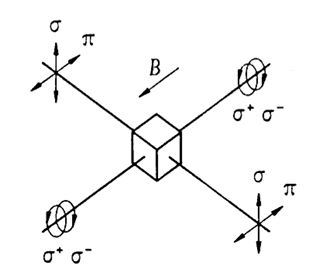
\includegraphics[width=0.5\textwidth]{Zeeman_effect_1.png}
    \caption{Illustration of the allowed transitions for the Zeeman effect, showing $\pi$-lines ($\Delta m_j = 0$) and $\sigma$-lines ($\Delta m_j = \pm 1$) for light propagating perpendicular to the magnetic field. Note that there is no $\pi$-line for light propagating parallel to the magnetic field because the magnetic dipole is oriented along the field. \cite{phyweZeeman}}
    \label{fig:zeeman_effect_1}
\end{figure}

\subsection{Normal and Anomalous Zeeman Effect}
The primary distinction between the normal and anomalous Zeeman effects lies in the electron spin. For the normal Zeeman effect, the electron spin $s = 0$, whereas for the anomalous Zeeman effect, $s \neq 0$. 

In terms of transitions, the initial state can be represented as $\mid i \rangle = \mid \ell_i, s_i, j_i, m_{j_i} \rangle$, and the final state as $\mid f \rangle = \mid \ell_f, s_f, j_f, m_{j_f} \rangle$. In our experiment, we use cadmium, and the specific transitions for the normal and anomalous Zeeman effects are as follows:
\begin{align}
    \text{Normal: } & \, 3^1\mathrm{D_2} \to 2^1\mathrm{P_1} \quad \text{or} \quad \mid 3; 2, 0, 2, m_j \rangle \to \mid 2; 1, 0, 1, m_j \rangle, \\
    \text{Anomalous: } & \, 2^3\mathrm{S_1} \to 2^3\mathrm{P_2} \quad \text{or} \quad \mid 2; 0, 1, 1, m_j \rangle \to \mid 2; 1, 1, 2, m_j \rangle.
    \label{eq:zeeman_transitions}
\end{align}
Indeed this form of transition representation loses the information of quantum number $m_j$. However, that's a not a big deal since later we only care about the $\Delta m_j$. So going back to the enegry difference between transions, we can use eq.\ref{eq:zeeman_energy} to calculate the energy difference between the two transitions as:
\begin{align}
    \Delta E &= \Delta E_0 + \mu_B B \biggl[ g_{j_f} m_{j_f} - g_{j_i} m_{j_i} \biggr], \,
    \begin{cases}
        \Delta m_{j} = m_{j_f} - m_{j_i} = 0, \, \text{for } \pi \text{-line} \\
        \Delta m_{j} = m_{j_f} - m_{j_i} = \pm 1, \, \text{for } \sigma_{\pm} \text{-line}
    \end{cases}
\end{align}
with the plotting corresponding quantum number in Eq.~\ref{eq:zeeman_transitions}, we have,
\begin{align}
    \begin{cases} 
        \text{Normal: } g_{j_f} = g_{j_i} = 1, \, \Delta m_j = m_{j_f} - m_{j_i}, \\
        \text{Anomalous: } g_{j_i} = 2, \, g_{j_f} = \frac{3}{2}
    \end{cases}
\end{align}
\indent Then we can summarize the transitions in Fig.~\ref{fig:zeeman_comparison}.

\begin{figure}[H]
    \centering
    \begin{subfigure}[b]{0.45\textwidth}
        \centering
        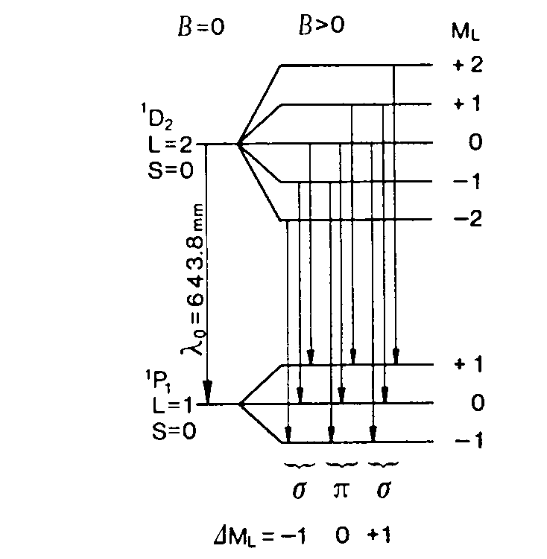
\includegraphics[width=\textwidth]{Normal_Zeeman.png}
        \caption{Normal Zeeman Transitions}
        \label{fig:normal_zeeman}
    \end{subfigure}
    \hfill
    \begin{subfigure}[b]{0.45\textwidth}
        \centering
        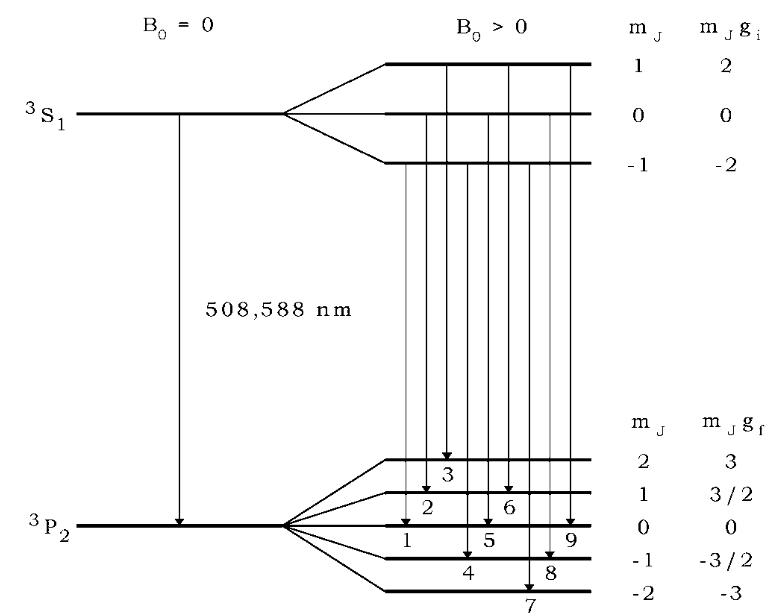
\includegraphics[width=\textwidth]{Anomalous_Zeeman.png}
        \caption{Anomalous Zeeman Transitions}
        \label{fig:anomalous_zeeman}
    \end{subfigure}
    \caption{Transitions we use for cadmium in our experiment. Theoretically, there are nine possible transition states for both effects. However, after passing through the Fabry-Perot Étalon, some transitions fail to exist.\cite{phyweZeeman}}
    \label{fig:zeeman_comparison}
\end{figure}
\subsection{Fabry-Perot Etalon: Frequency Selection}
The Fabry-Perot etalon is a critical component in our experiment, used to select specific frequencies from the light emitted by the cadmium lamp. Since the light source is not monochromatic, the etalon ensures that only the desired spectral lines are transmitted for analysis.

The etalon consists of two parallel, partially reflecting mirrors separated by a distance $d$. Light waves reflect back and forth between the mirrors, creating an interference pattern. The condition for constructive interference is given by:
\begin{equation}
    2\mu t\cos \theta = n \lambda,
\label{eq:fabry_perot_condition}
\end{equation}
where $t$ is the separation between the mirrors, $\theta$ is the angle of incidence, $n$ is the interference order, $\mu$ is the reflective index in quartz, and $\lambda$ is the wavelength of the transmitted light. 


Figure \ref{fig:fabry_perot_interference} illustrates the working principle of the Fabry-Perot etalon. Light entering the etalon at an angle $\theta$ undergoes multiple reflections, and only wavelengths satisfying the interference condition (eq.\ref{eq:fabry_perot_condition}) emerge constructively. Thus we have:
\begin{equation}
    n = \frac{2\mu t}{\lambda} \cos \theta_n = n_0 \cos \theta_n, \quad \text{where } n_0 = \frac{2\mu t}{\lambda}.
\end{equation}

\begin{equation}
    \theta_n = \sqrt{\frac{2(n_{0}-n)}{n_{0}}}
\end{equation}
\begin{figure}[H]
    \centering
    \begin{subfigure}[b]{0.45\textwidth}
        \centering
        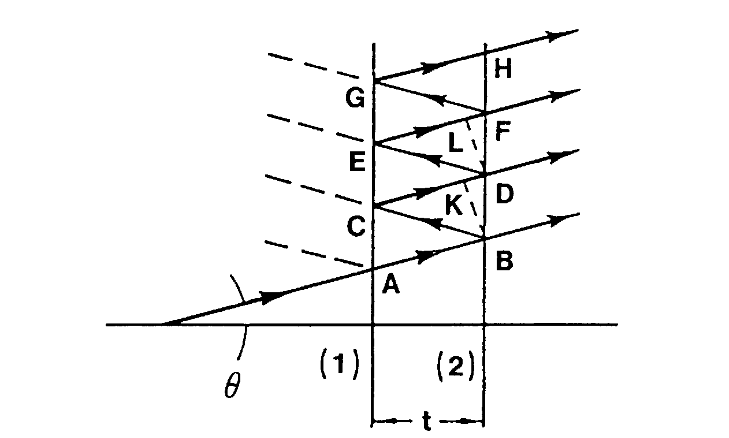
\includegraphics[width=\textwidth]{fabry_perot_2.png}
        \caption{Reflected and transmitted rays at the parallel surfaces.}
        \label{fig:fabry_perot_interference}
    \end{subfigure}
    \hfill
    \begin{subfigure}[b]{0.45\textwidth}
            \centering
            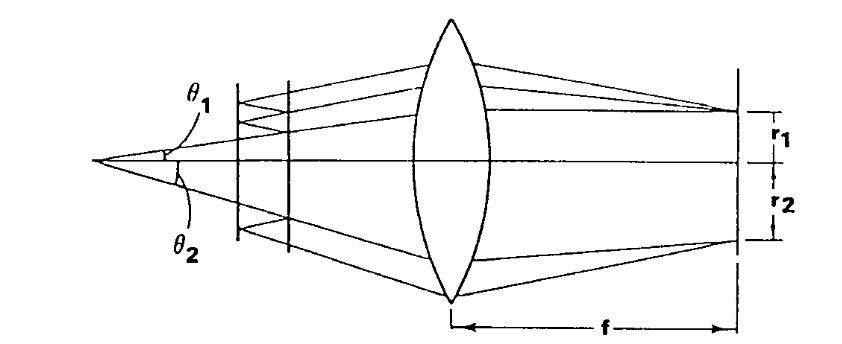
\includegraphics[width=\textwidth]{fabry_perot_1.png}
            \caption{Ring radius on the analyser is $r = f\theta$, where $f$ is the focal length of the lens.}
            \label{fig:fabry_perot_focusing}
        \label{fig:fabry_perot_focusing}
    \end{subfigure}
    \label{fig:fabry_perot_diagram}
\end{figure}
\indent And since $n_1 < n_0$ and $n_1 = n_0 \cos \theta$, we can let:
\begin{equation}
    n_1 = n_0 - \epsilon \quad ; 0<\epsilon < 1
\end{equation}
\indent And for the pth order of interference, we have:
\begin{equation}
    n_p = (n_0 - \epsilon) - (n_p -1)
\end{equation}
\indent We can see in figure \ref{fig:fabry_perot_focusing} that the light rays are focused on the analyser. With small angle approximation, we can write the radius of the ring on the analyser as:
\begin{equation}
    r = f \tan\theta \approx f \theta
    \label{eq:fabry_perot_radius}
\end{equation}
\indent Therefore, combining eq.\ref{eq:fabry_perot_condition} and eq.\ref{eq:fabry_perot_radius}, we can get the difference on radius of the ring on the analyser as:
\begin{equation}
     r^2_{p+1} - r^2_{p} = 2 \frac{f^2}{n_0}, ~~~\,\text{with}\, r_p = \sqrt{\frac{2f^2}{n_0}} \cdot \sqrt{(p-1) + \epsilon} 
    \label{eq:fabry_perot_radius_diff}
\end{equation}
\indent Now if there are two different wavelengths $\lambda_a$ and $\lambda_b$ in the light source, we can write the $n_0$ for both wavelengths respect to its corresponding wave number $k_a$ and $k_b$ as:
\begin{align}
    \begin{cases}
        \epsilon_a &= \frac{2\mu \cdot t}{\lambda_a} = -n_{1,a} = 2\mu \cdot t \cdot k_a - n_{1,a}, \\
        \epsilon_b &= \frac{2\mu \cdot t}{\lambda_b} = -n_{1,b} = 2\mu \cdot t \cdot k_b - n_{1,b}.
    \end{cases}
    \label{eq:fractional_orders}
\end{align}
\indent Then combining eq.\ref{eq:fabry_perot_radius_diff} and eq.\ref{eq:fractional_orders}, we can get the difference of wave number $k$ as:
\begin{align}
    \Delta k &= k_a - k_b = \frac{1}{2\mu \cdot t} \biggl[ \frac{r_{p+1,a}^2}{r_{p+1,b}^2 - r_{p,a}^2} - \frac{r_{p+1,b}^2}{r_{p+1,b}^2 - r_{p,b}^2} \biggr]
    \label{eq:wave_number_diff}
\end{align}
\indent From the relation in eq.\ref{eq:fabry_perot_radius}, we can assume for $n_{0,b} \approx n_{0,a}$ we have:
\begin{equation}
    \Delta^{p+1,p}_{a} = r^2_{p+1} - r^2_{p,a} = 2 \frac{f^2}{n_{0,a}} = \Delta^{p+1,p}_{b} = r^2_{p+1} - r^2_{p,b} = 2 \frac{f^2}{n_{0,b}}
\end{equation}
\indent and for all value of $p$ we have: 
\begin{equation}
    \delta^{p}_{a} = r^2_{p+1,a} - r^2_{p+1,a} 
\end{equation}
\indent Thus, we rewrite eq.\ref{eq:wave_number_diff} as(assuming $\Delta E_0 = 0$):
\begin{equation}
    \Delta k = \frac{1}{2\mu \cdot t}\cdot\frac{\delta}{\Delta}
    \label{eq:wave_number_diff_final}
\end{equation}
\indent From the above we can reqrite the energy differnce in terms of $\Delta k$:
\begin{equation}
    \Delta E = \mu_B B \biggl[ g_{j_f} m_{j_f} - g_{j_i} m_{j_i} \biggr] =  \hbar c \Delta k = \frac{\hbar c}{2\mu \cdot t} \cdot \frac{\delta}{\Delta}
    \label{eq:energy_diff_final}
\end{equation}
To summarize, we can see the possible rings in given $p$ in table.\ref{tab:ZeemanComparison}
\begin{table}[ht]
    \centering
    \renewcommand{\arraystretch}{1.2}
    \begin{tabular}{c|c|c}
    \hline
     & (a) $\Delta\bigl(g_j m_j\bigr)$ 
     & (b) Possible rings for a fixed order \\
    \hline
    \textbf{Normal} 
     & \begin{tabular}{@{}l@{}}
       $\sigma(\Delta m_j = +1): \{+1,+1,+1\}$\\
       $\sigma(\Delta m_j = -1): \{-1,-1,-1\}$\\
       $\pi(\Delta m_j = 0): \{0,0,0\}$\\
       \end{tabular}
     & \begin{tabular}{@{}l@{}}
       \textit{Transverse}: 1 + 2 rings \\
       \textit{Longitudinal}: 0 + 2 rings
       \end{tabular}
    \\
    \hline
    \textbf{Anomalous} 
     & \begin{tabular}{@{}l@{}}
       $\sigma(\Delta m_j = +1): \{2,\tfrac{3}{2},1\}$\\
       $\sigma(\Delta m_j = -1): \{-\tfrac{3}{2},-1,-\tfrac{1}{2}\}$\\
       $\pi(\Delta m_j = 0): \{\tfrac{1}{2},0,-\tfrac{1}{2}\}$\\
       \end{tabular}
     & \begin{tabular}{@{}l@{}}
       \textit{Transverse}: 3 + 6 rings \\
       \textit{Longitudinal}: 0 + 6 rings
       \end{tabular}
    \\
    \hline
    \end{tabular}
    \caption{(a) The value of $\Delta\bigl(g_j m_j\bigr)$ for normal and anomalous Zeeman effects, and 
    (b) the corresponding number of rings in the Fabry--Perot interference pattern for a fixed order with the left number representing $\pi$-line and right number representing $\sigma_{\pm}$.}
    \label{tab:ZeemanComparison}
    \end{table}
    

\section{Experiment Setup and Procedure}
\subsection{Experimental Setup}
The electromagnet is placed on a rotating table designed for heavy loads and is mounted with two pole-pieces that have holes, leaving a gap (9--11~mm) large enough for the Cd-lamp. The pole-pieces must be tightened securely. The Cd-lamp is inserted into the gap without touching the pole-pieces and is connected to the power supply for spectral lamps.

The scheme of the set up can be shown in figure.\ref{fig:setup}.
\begin{figure}[H]
    \centering
    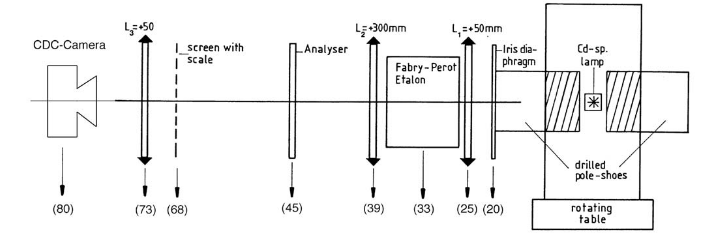
\includegraphics[width=0.8\textwidth]{setup.png}
    \caption{Experimental setup for observing the Zeeman effect. The optical bench is equipped with a lens system, a Fabry-Perot étalon, and a CCD camera for capturing the interference pattern.}
    \label{fig:setup}
\end{figure}
\subsection{Procedure}
    1. First we open the cadmium light and put on the red light filter make sure that the fringes on the CCD is center at the center of the screen. \\
\indent 2. Then we adjust the Fabry-Perot etalon to get the best interference pattern. The etalon is adjusted by rotating the two screws on the side of the etalon. The best interference pattern is achieved when the rings are sharp and well-defined. We also change focals and exposure of the CCD to get the best resolution\\
\indent 3. After that we took picture of the polarization entering the CCD at 0\textdegree, 90\textdegree, and 180\textdegree\\ 
\indent 4. Then we rotate the electromagnet by 90\textdegree, insert quarter waveplate and replace the red light filter with green light filter for longitudinal observation.\\
\indent 5. We repeat the same procedure as above to get the best interference pattern.\\
\indent 6. After that we took picture of the polarization entering the CCD at 0\textdegree, 90\textdegree, and 180\textdegree\\

\subsection{Transversal Observation}
    After completing the initial adjustments, the electromagnet is rotated by 90\textdegree, and the iris diaphragm is inserted for transversal observation.
    
    \subsection{Calibration Remark}
    For later evaluations, a calibration curve of the magnetic flux density versus the coil current must be recorded. This can be performed using a teslameter. If unavailable, the results shown in Fig.~3 can be used. Note that the flux density measured in the center of the gap (in the absence of the Cd-lamp) should be increased by 3.5\% to account for the non-uniform flux distribution within the gap.
    
    % End of Section 3
    

    \section{Data Analysis }

    \subsection{Observation of Zeeman Effect}
    
    \par Firstly we started by the observation of the transversal normal Zeeman effect and anomalous Zeeman effect, both with and without polarization, the observation is shown in Fig.\ref{fig:tra_nor} and Fig.\ref{fig:tra_ano} with the magnetic field fixed at $d=43 $ (mm).
    
    \begin{figure}[H]
        \centering
        \begin{subfigure}[b]{0.3\textwidth}
            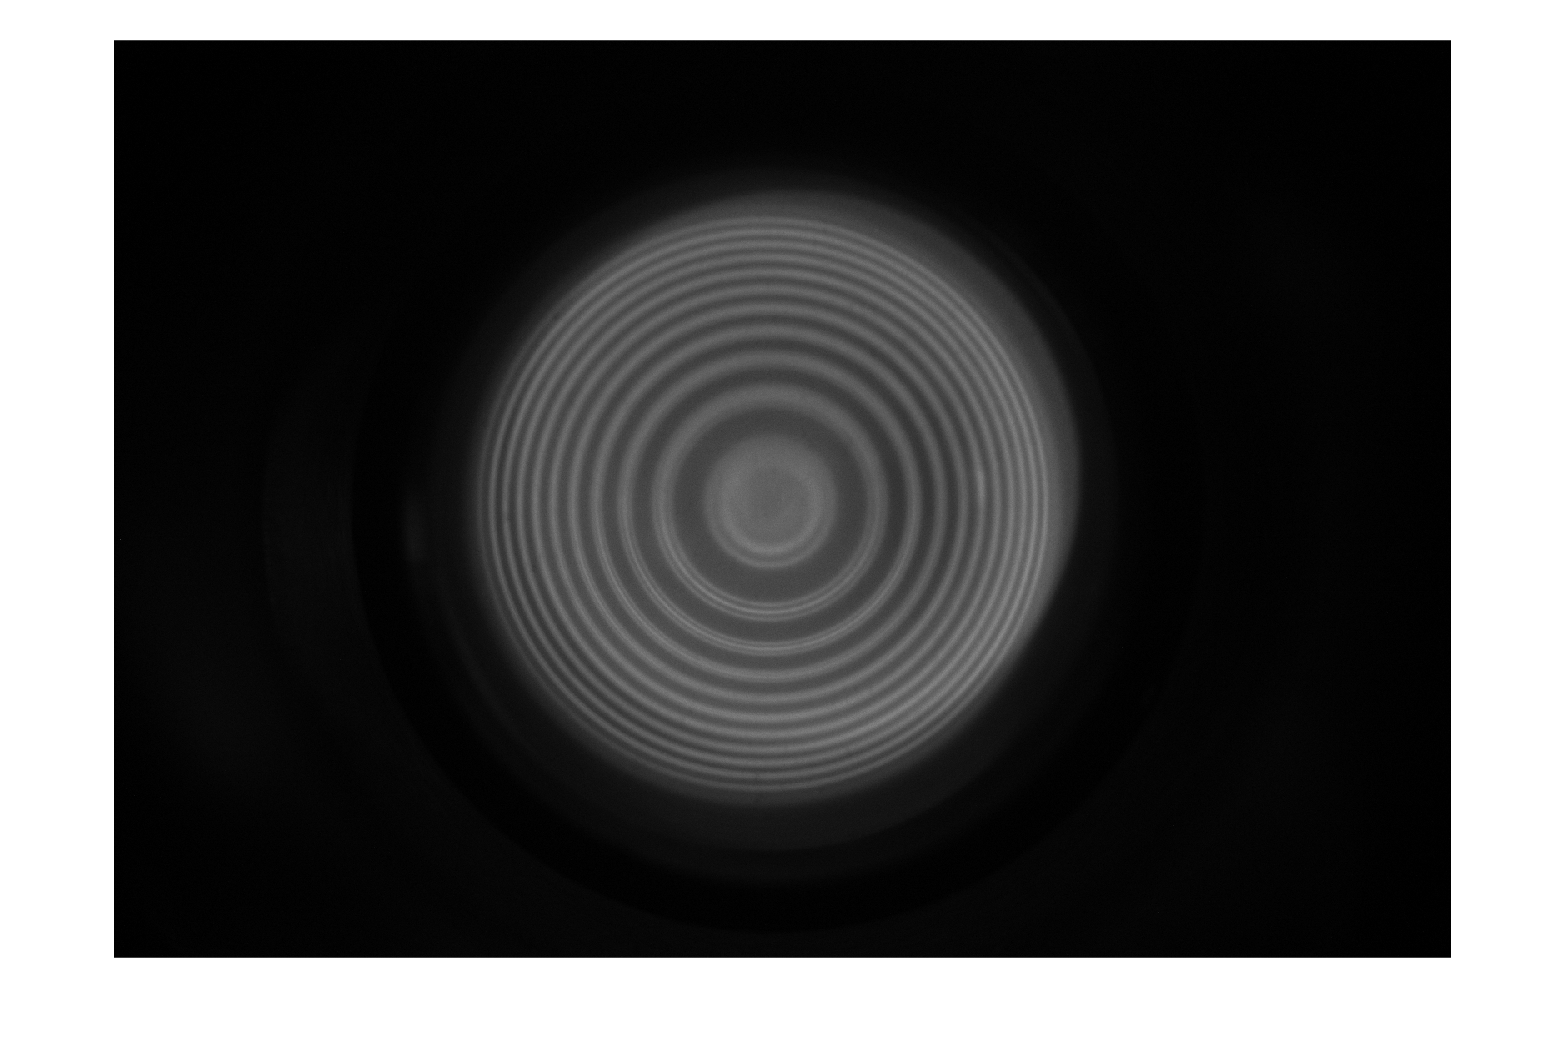
\includegraphics[width=1.2\textwidth]{tra_nor_none.png}
            \caption{no polarization}
            % \label{fig:tra_nor_none}
        \end{subfigure}
        \space
        \begin{subfigure}[b]{0.3\textwidth}
            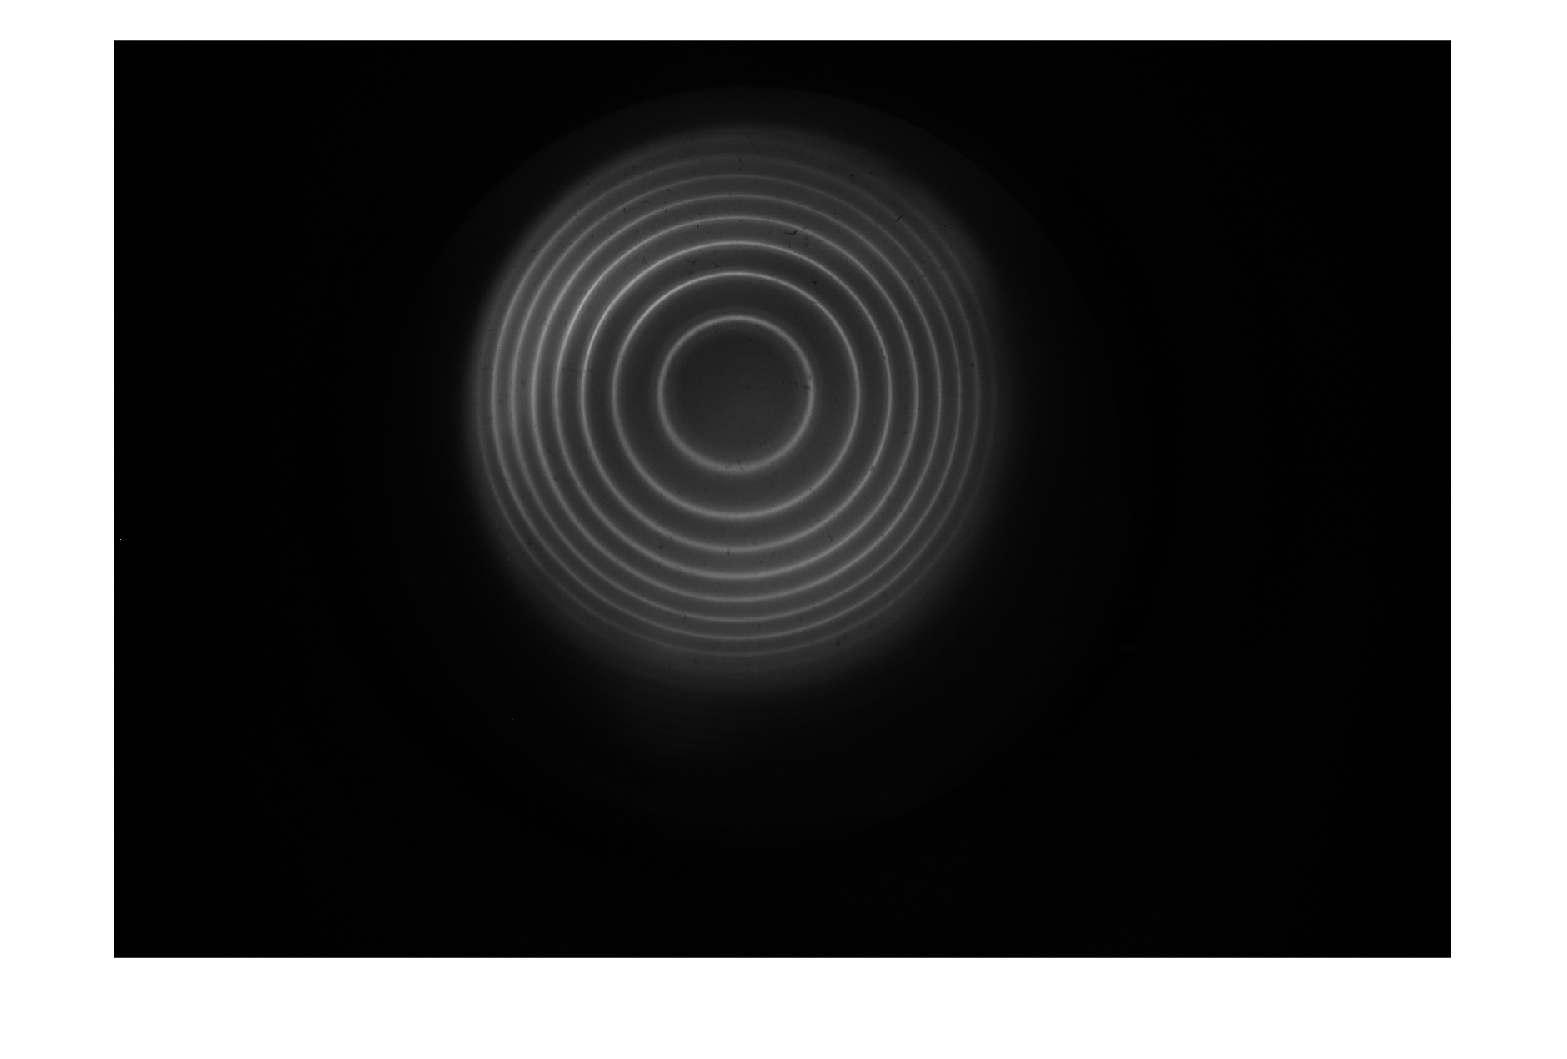
\includegraphics[width=1.2\textwidth]{tra_nor_hor.png}
            \caption{horizontal}
            % \label{fig:tra_nor_hor}
        \end{subfigure}
        \space
        \begin{subfigure}[b]{0.3\textwidth}
            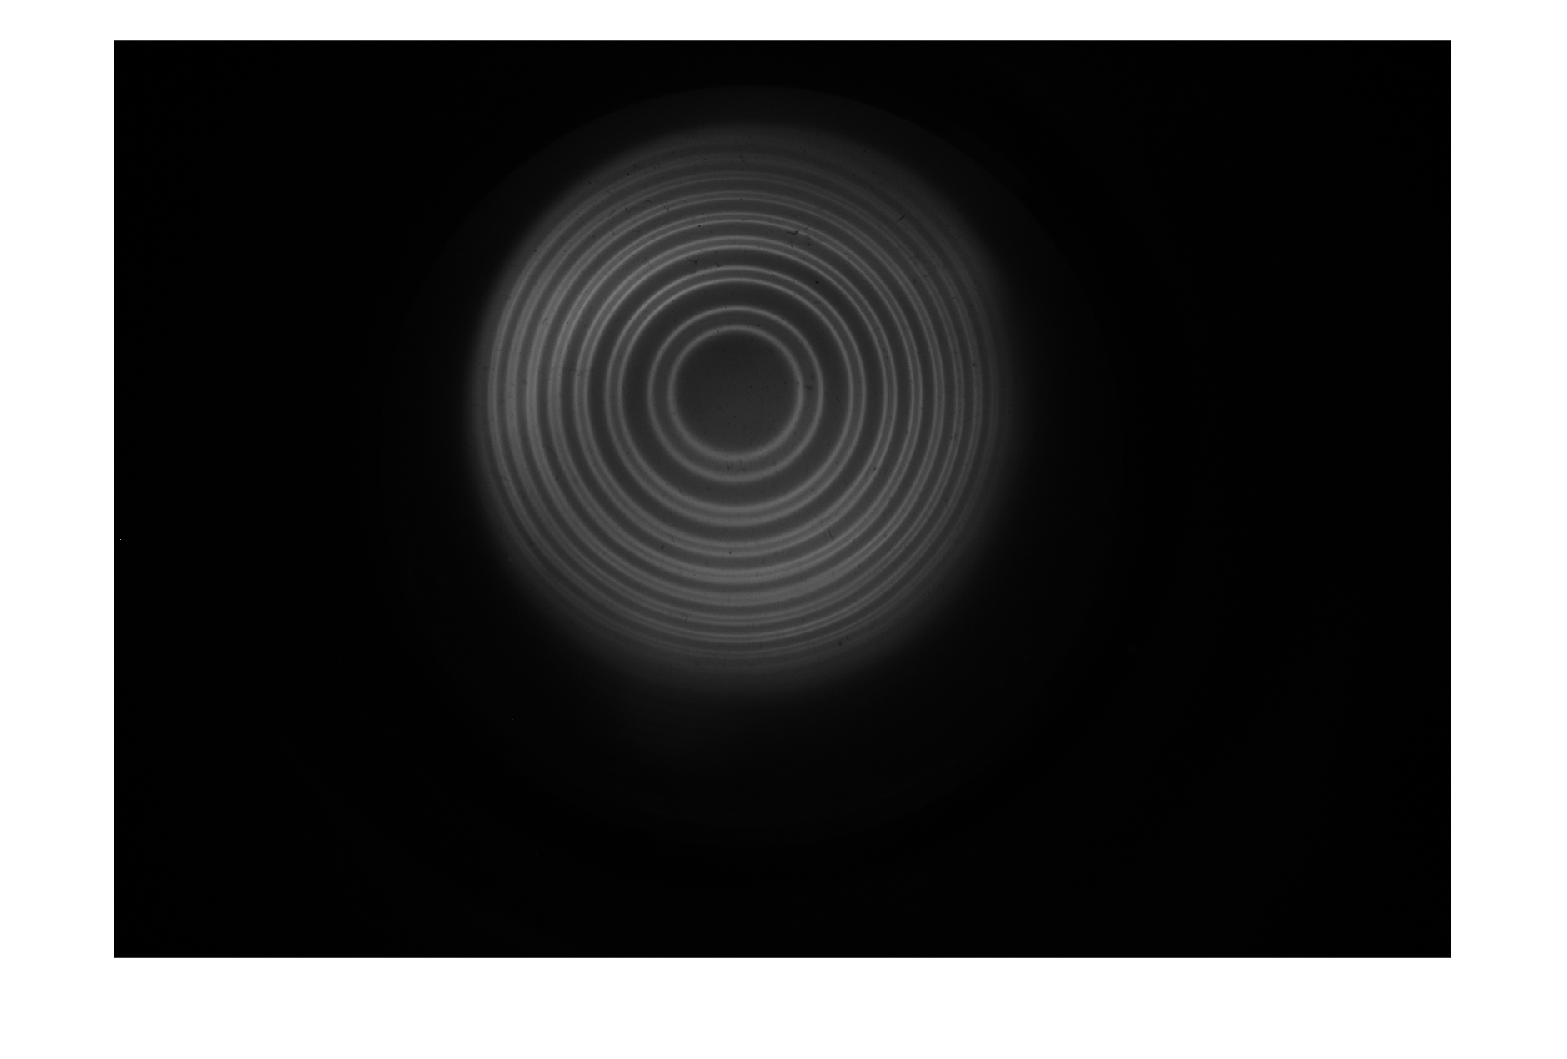
\includegraphics[width=1.2\textwidth]{tra_nor_ver.png}
            \caption{vertical}
            % \label{fig:tra_nor_ver}
        \end{subfigure}
        \caption{Transversal normal Zeeman effect.}
        \label{fig:tra_nor}
    \end{figure}
    
    \begin{figure}[H]
        \centering
        \begin{subfigure}[b]{0.3\textwidth}
            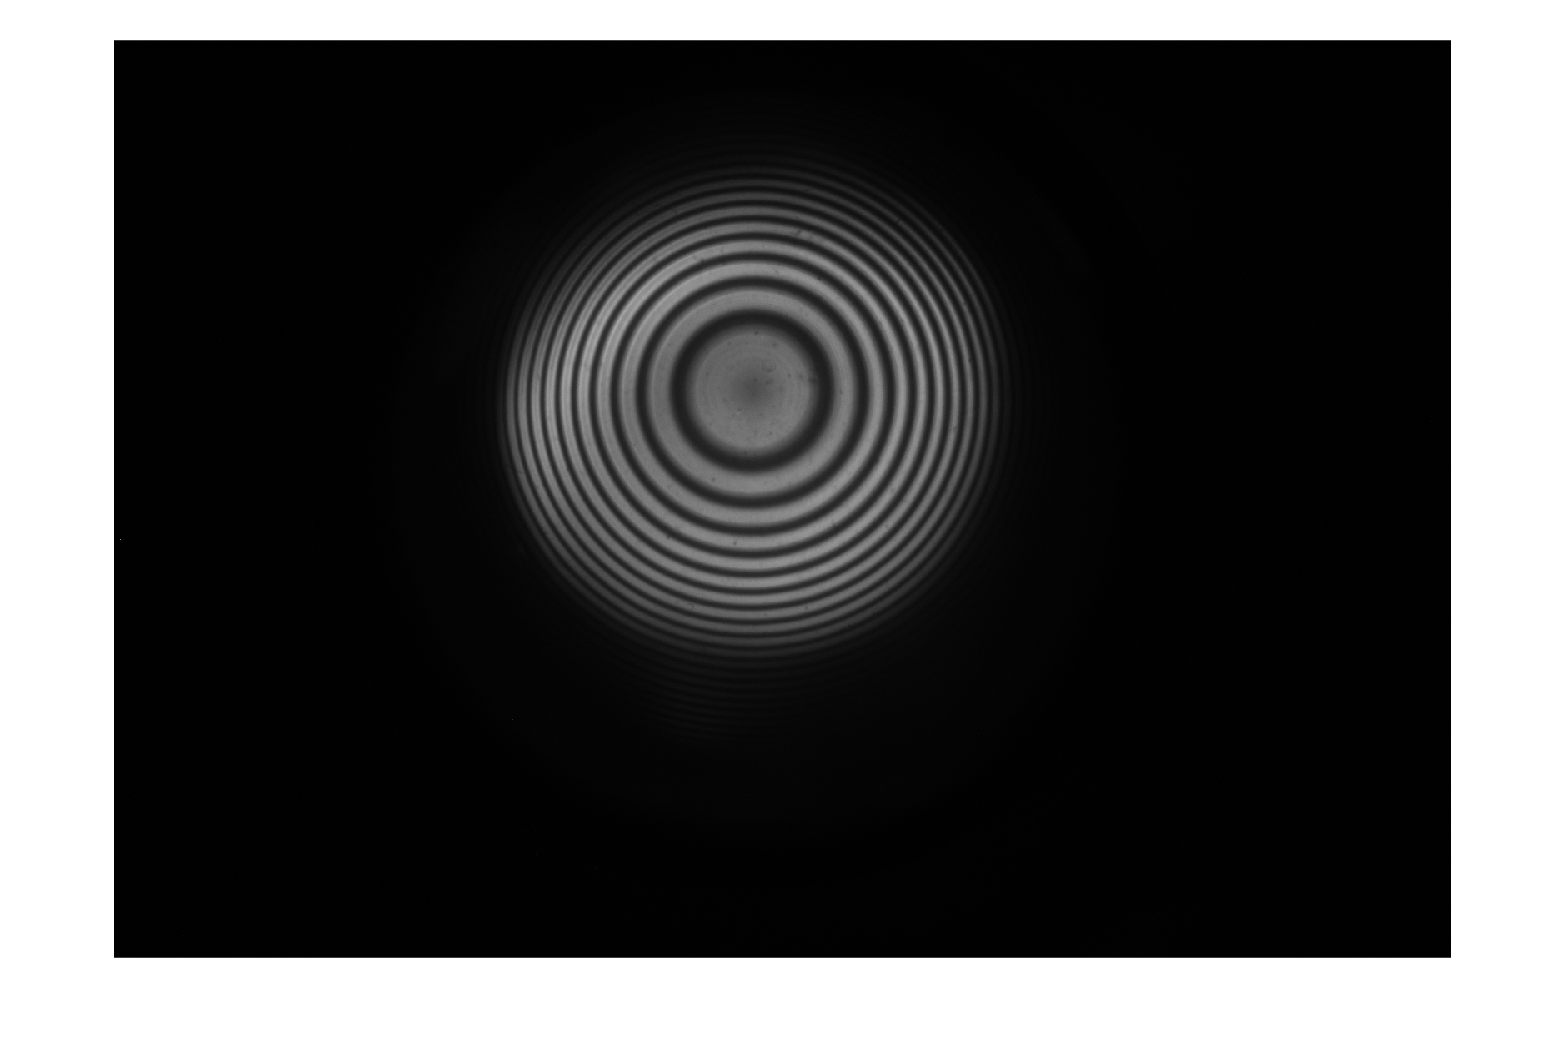
\includegraphics[width=1.2\textwidth]{tra_ano_none.png}
            \caption{no polarization}
        \end{subfigure}
        \space
        \begin{subfigure}[b]{0.3\textwidth}
            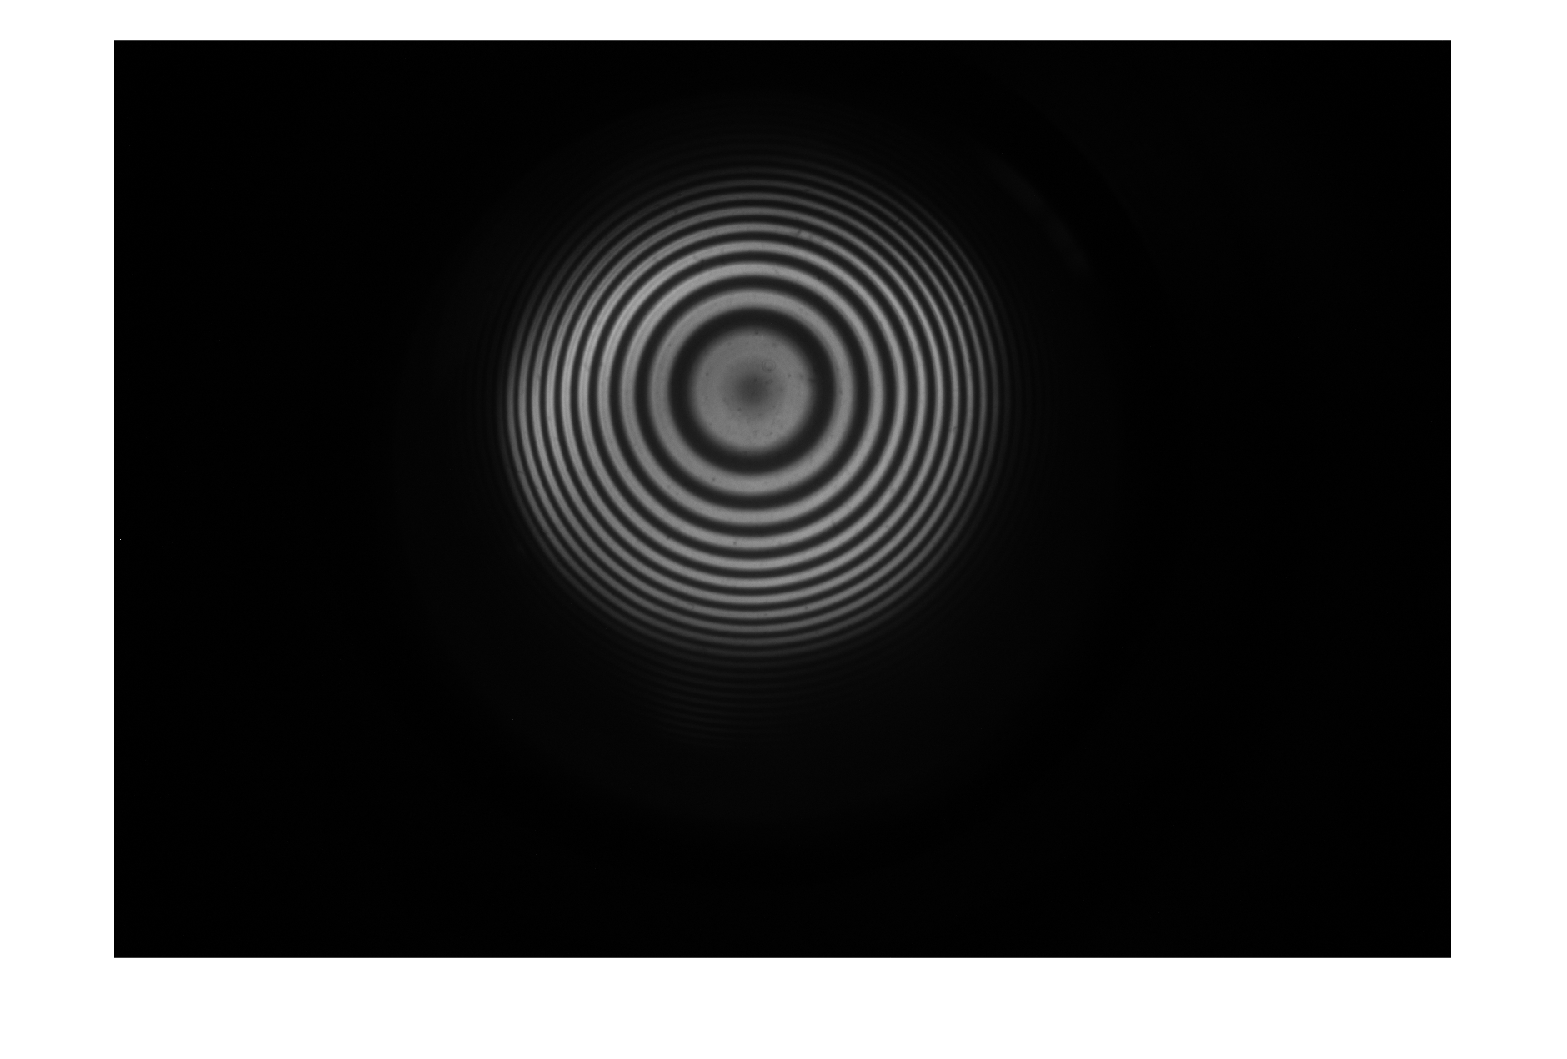
\includegraphics[width=1.2\textwidth]{tra_ano_hor.png}
            \caption{horizontal}
        \end{subfigure}
        \space
        \begin{subfigure}[b]{0.3\textwidth}
            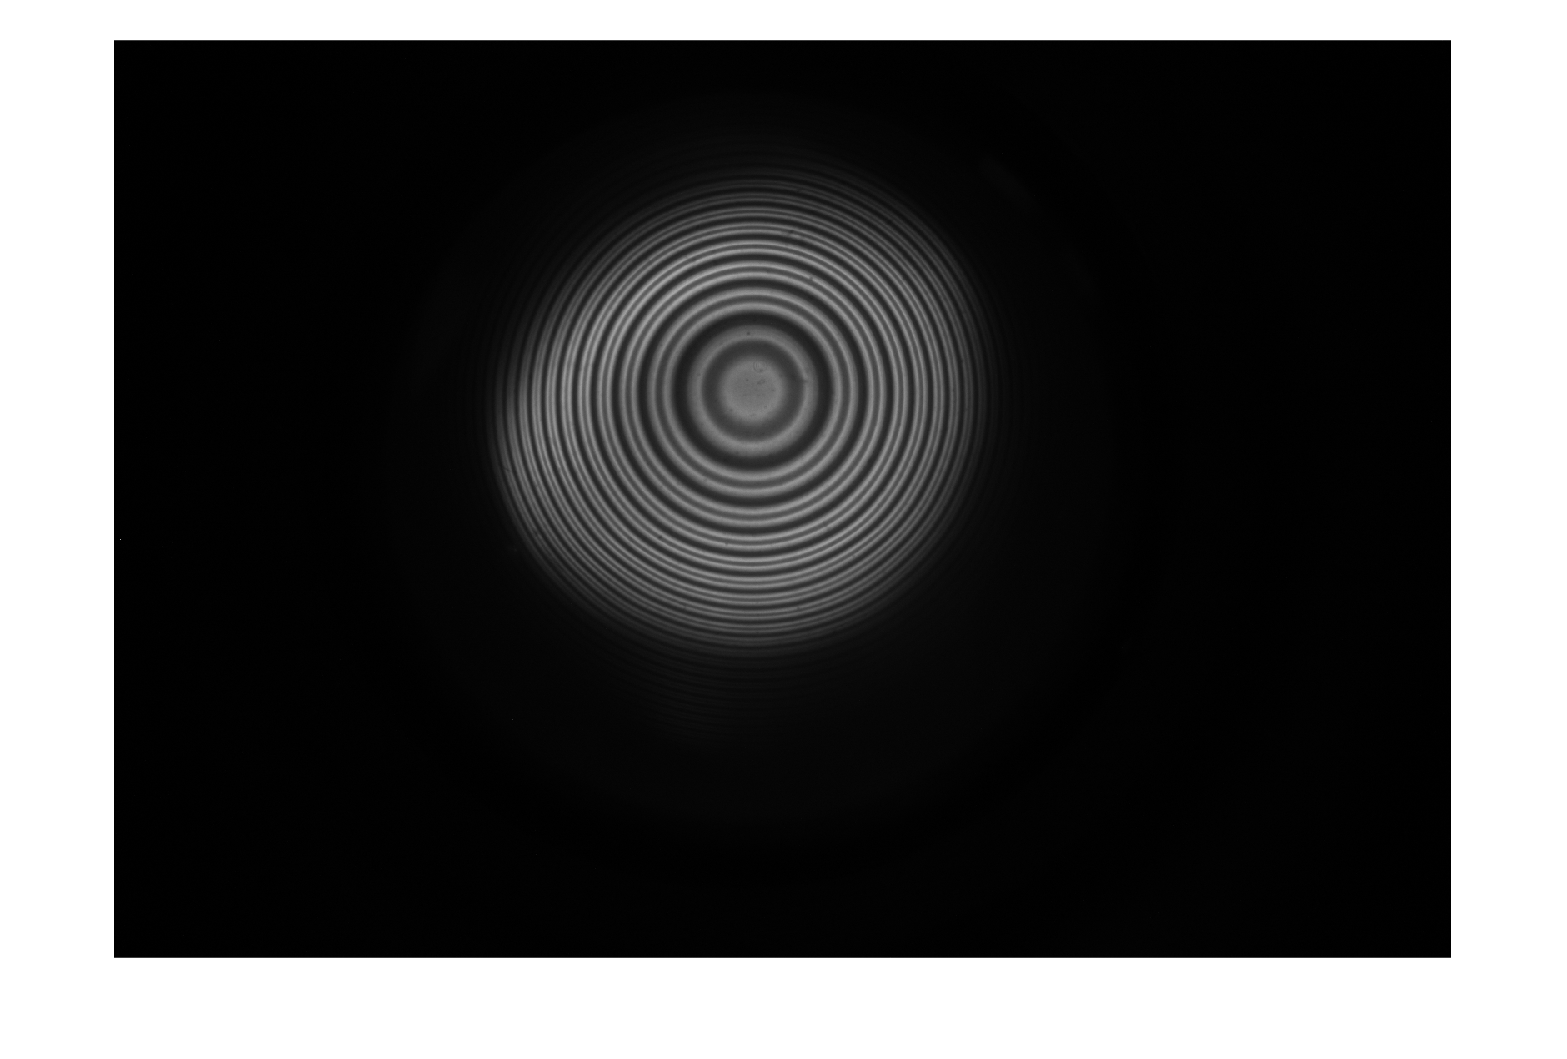
\includegraphics[width=1.2\textwidth]{tra_ano_ver.png}
            \caption{vertical}
        \end{subfigure}
        \caption{Transversal anomalous Zeeman effect.}
        \label{fig:tra_ano}
    \end{figure}
    
    \par Then we put the quarter-wave plate on and observe the longitudinal normal Zeeman effect and anomalous Zeeman effect, the observation is shown in Fig.\ref{fig:lon_nor} and Fig.\ref{fig:lon_ano} where the magnetic field is fixed at $d=43 $ (mm).
    
    \begin{figure}[H]
        \centering
        \begin{subfigure}[b]{0.3\textwidth}
            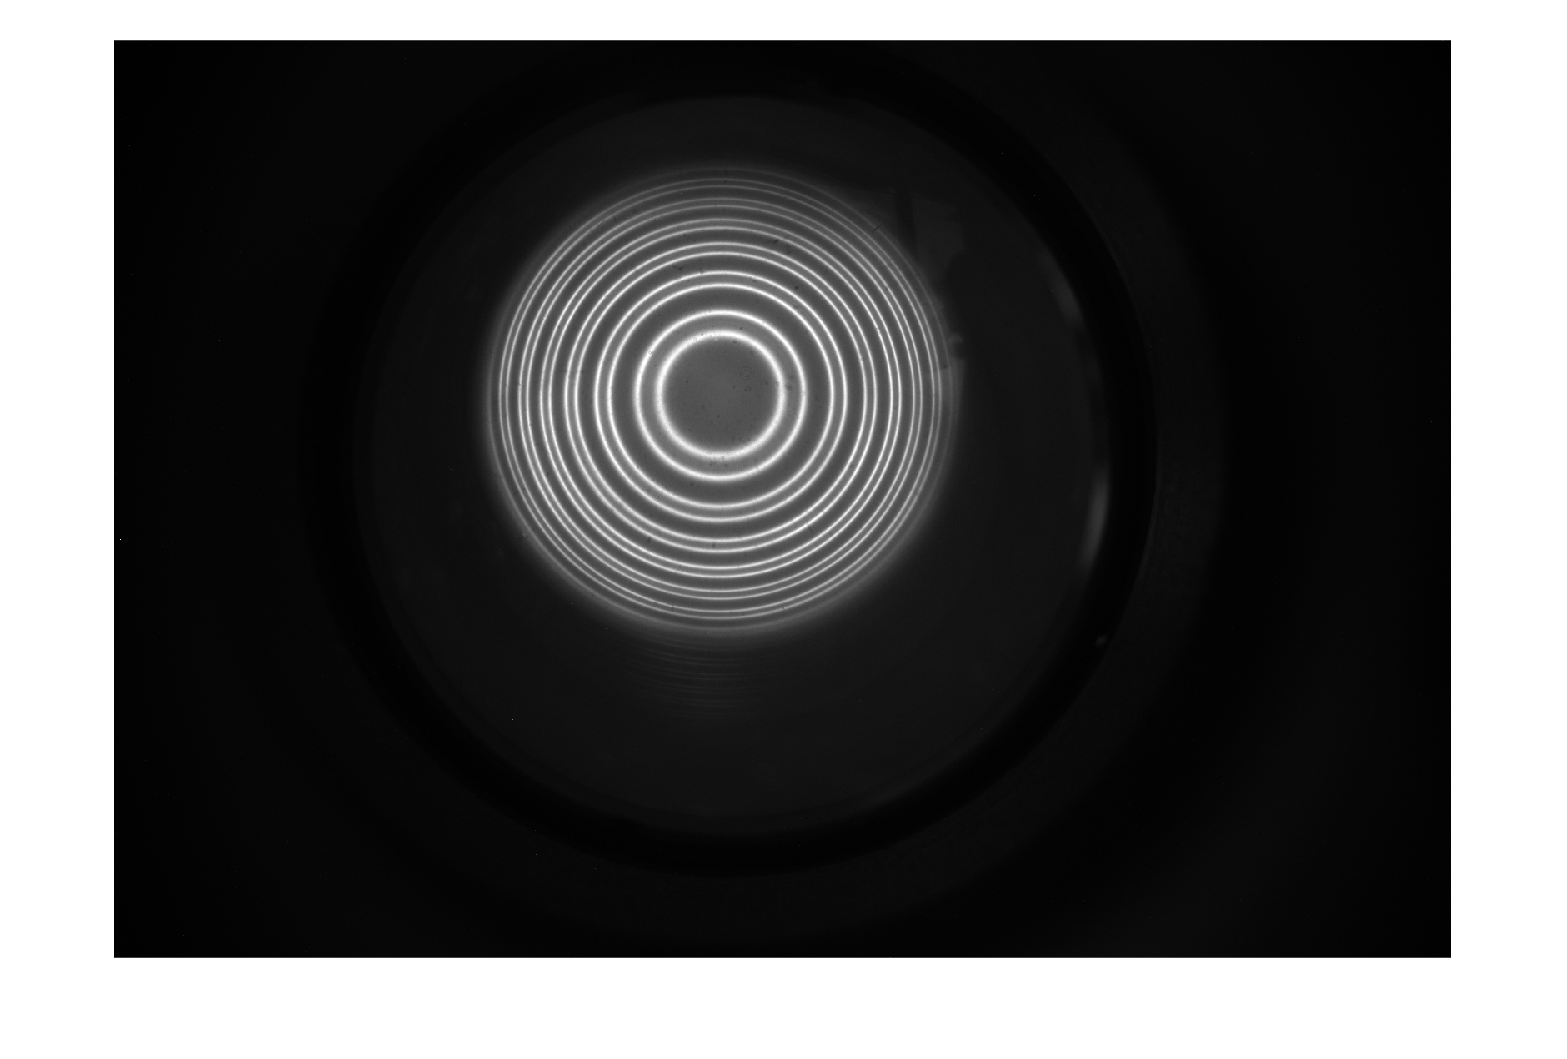
\includegraphics[width=1.2\textwidth]{lon_nor_none.png}
            \caption{no polarization}
        \end{subfigure}
        \space
        \begin{subfigure}[b]{0.3\textwidth}
            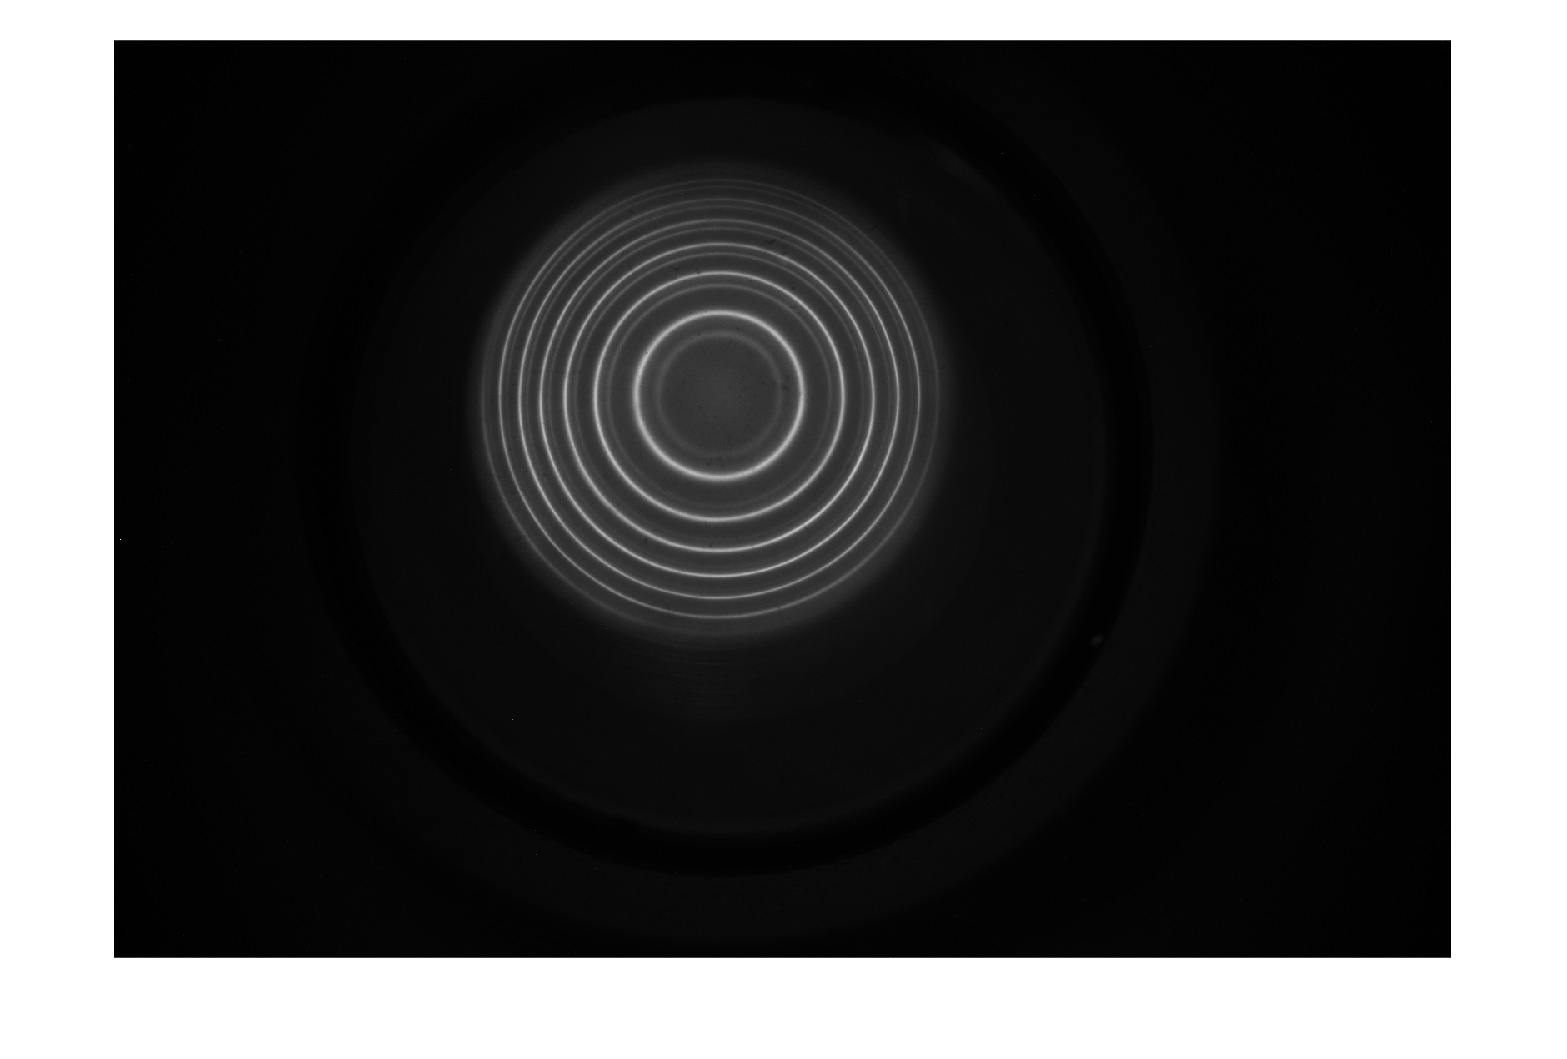
\includegraphics[width=1.2\textwidth]{lon_nor_45.png}
            \caption{45 degree}
        \end{subfigure}
        \space
        \begin{subfigure}[b]{0.3\textwidth}
            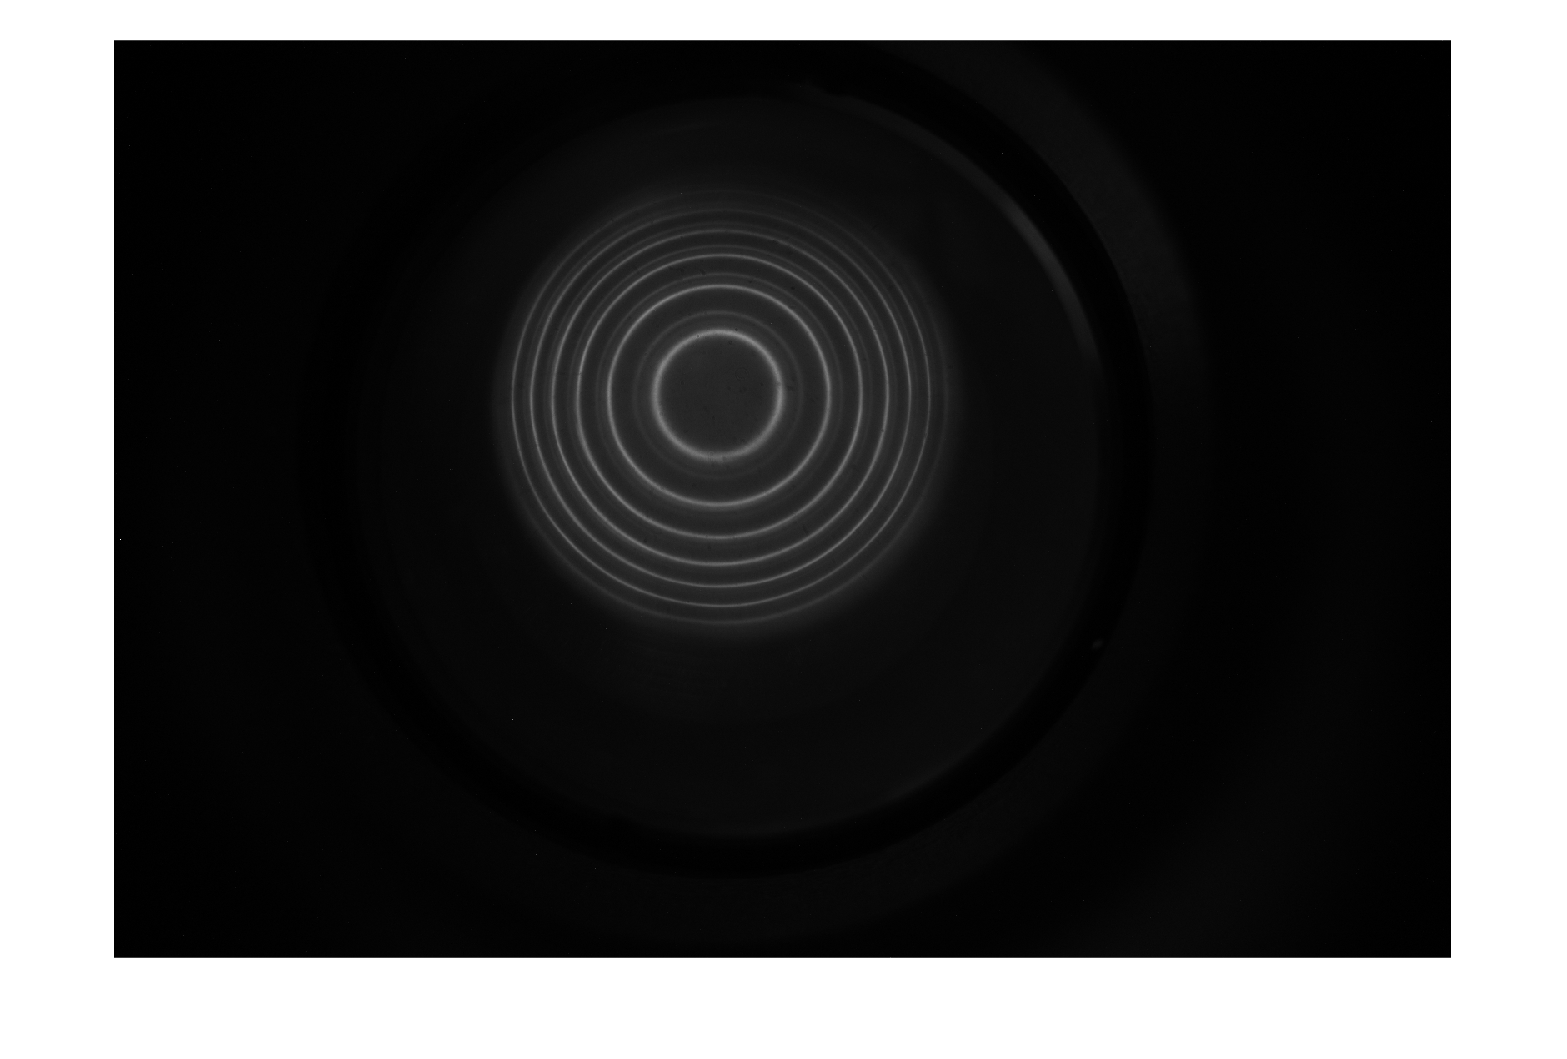
\includegraphics[width=1.2\textwidth]{lon_nor_-45.png}
            \caption{-45 degree}
        \end{subfigure}
        \caption{Longitudinal normal Zeeman effect.}
        \label{fig:lon_nor}
    \end{figure}
    
    \begin{figure}[H]
        \centering
        \begin{subfigure}[b]{0.3\textwidth}
            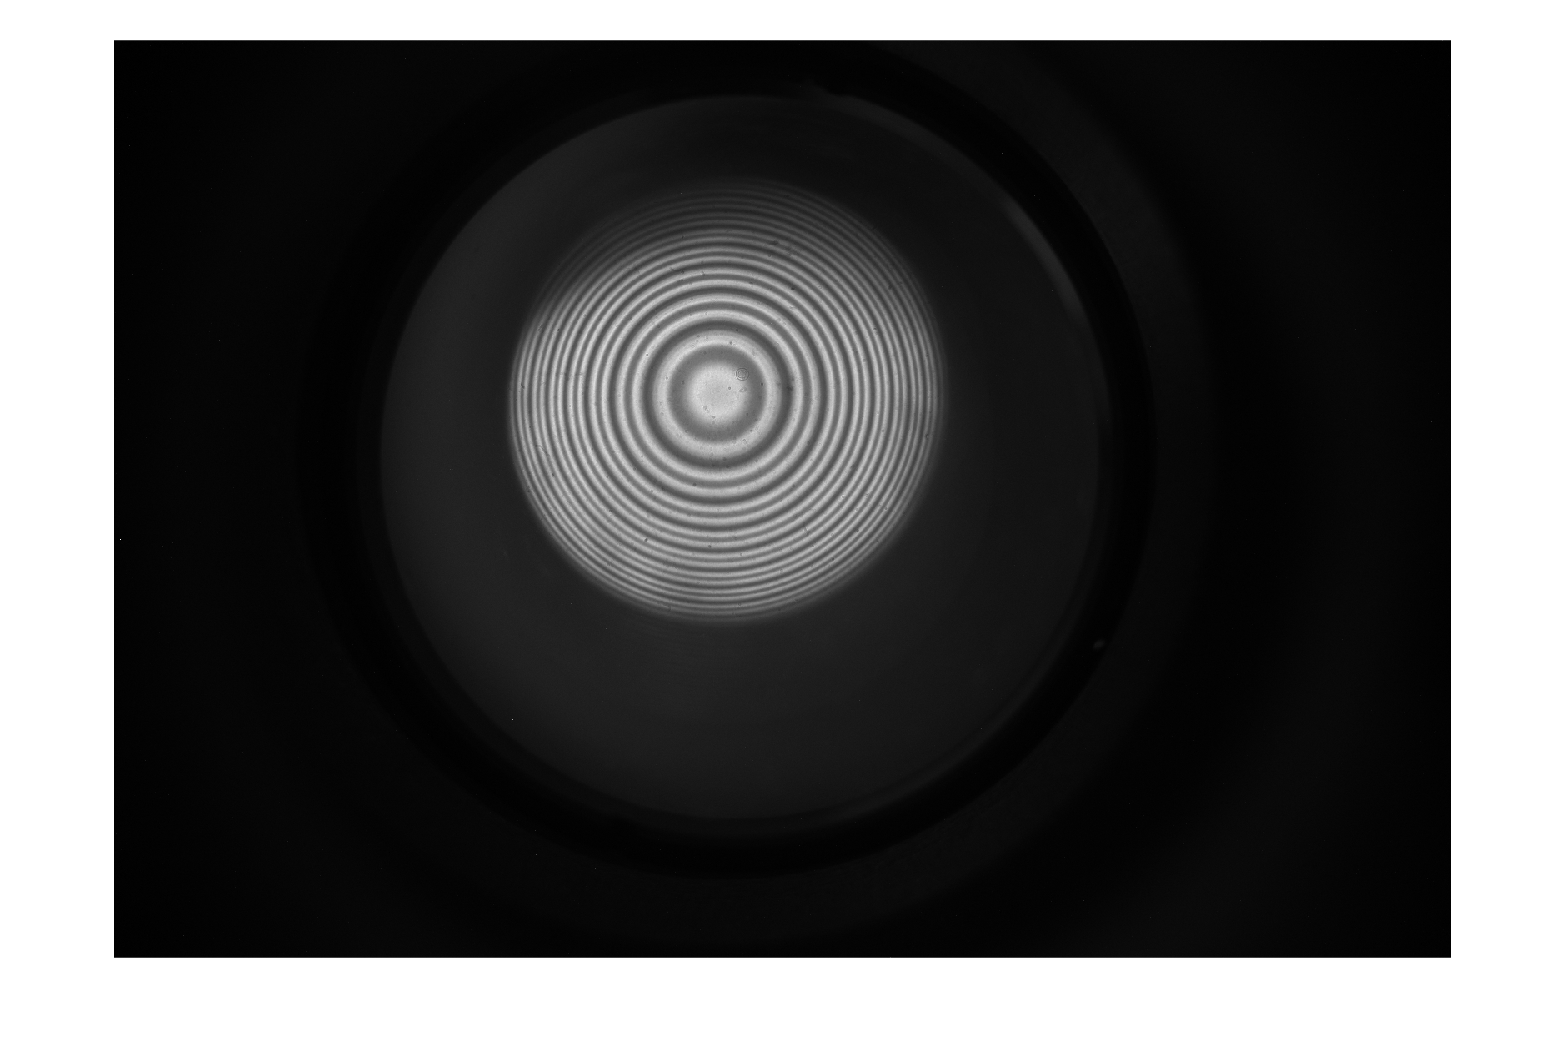
\includegraphics[width=1.2\textwidth]{lon_ano_none.png}
            \caption{no polarization}
        \end{subfigure}
        \space
        \begin{subfigure}[b]{0.3\textwidth}
            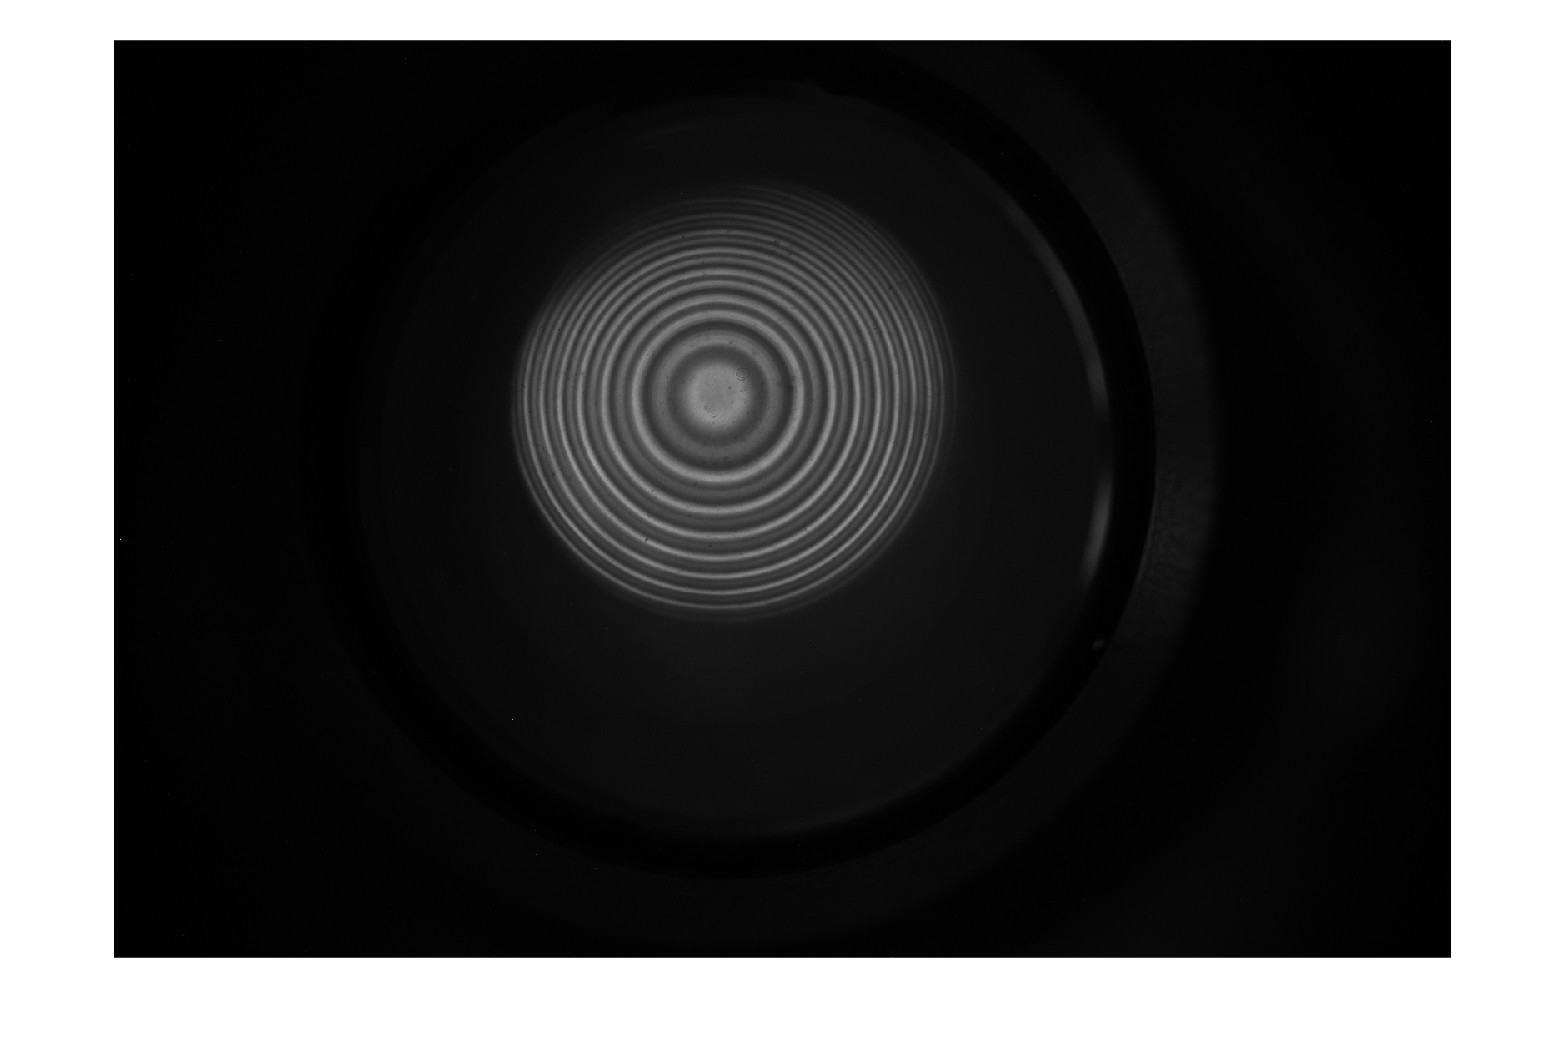
\includegraphics[width=1.2\textwidth]{lon_ano_45.png}
            \caption{45 degree}
        \end{subfigure}
        \space
        \begin{subfigure}[b]{0.3\textwidth}
            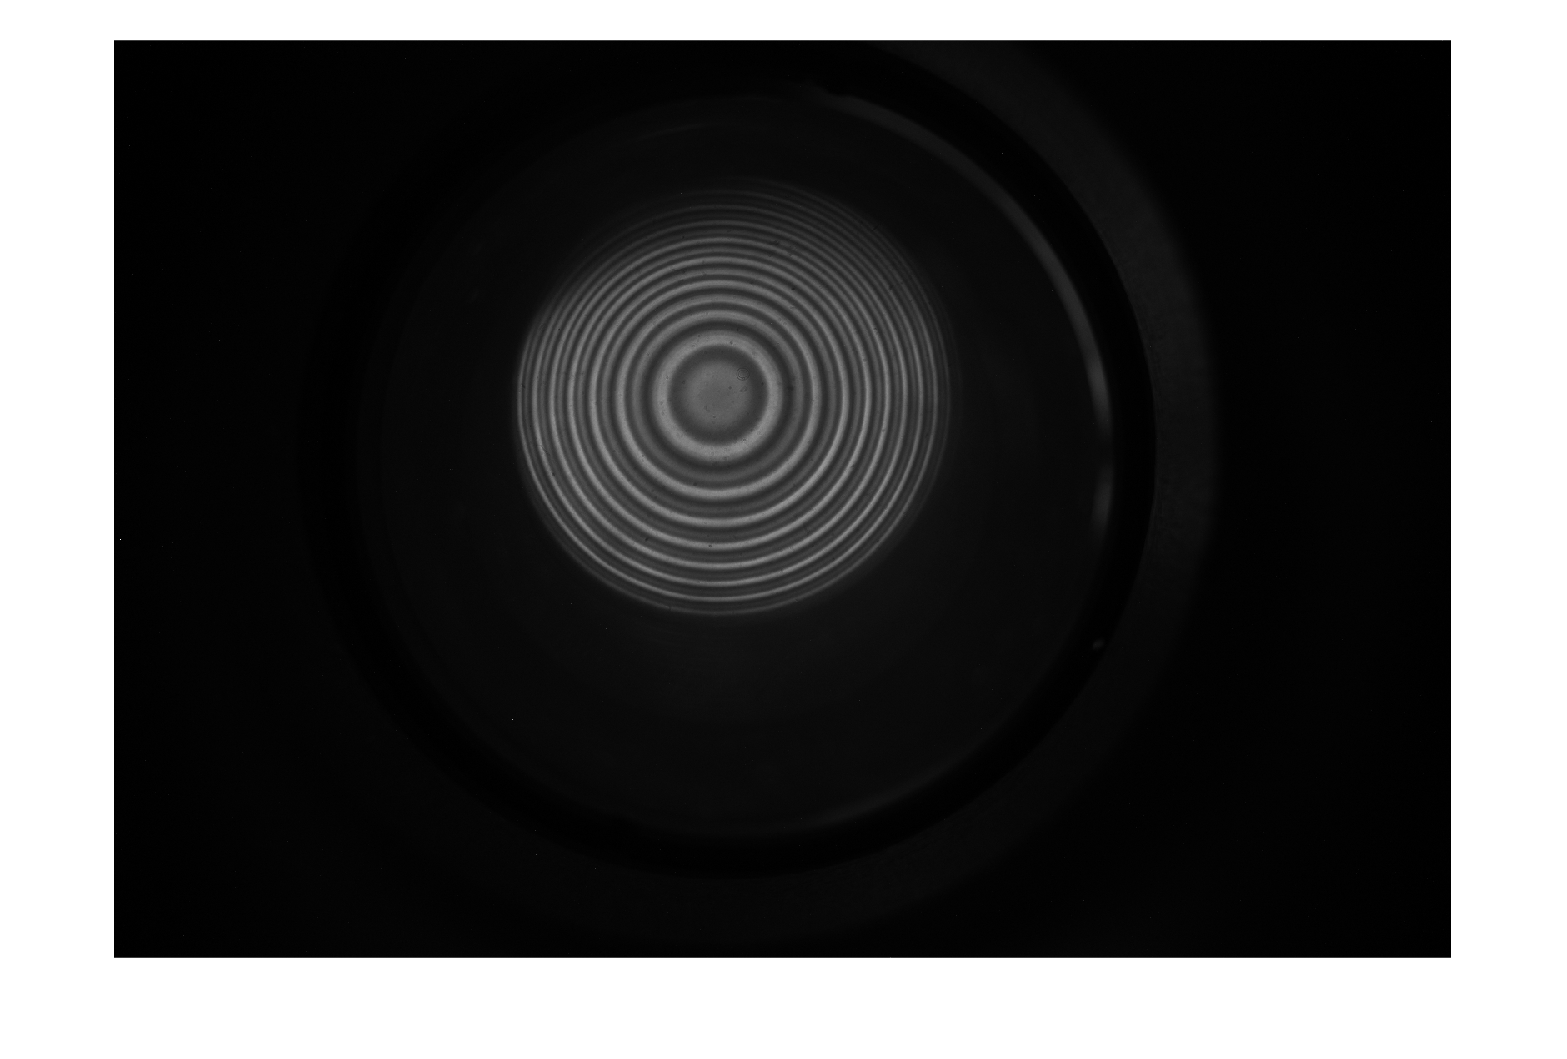
\includegraphics[width=1.2\textwidth]{lon_ano_-45.png}
            \caption{-45 degree}
        \end{subfigure}
        \caption{Longitudinal anomalous Zeeman effect.}
        \label{fig:lon_ano}
    \end{figure}
    
    \par We can see all the splitting spectral lines from the non-polarization situation, and we apply different polarization to separate the $\pi$, $\sigma$ lines for the transversal Zeeman effect, while for the longitudinal Zeeman effect we apply the 45 degree and -45 degree polarization to separate the $\sigma^+$, $\sigma^-$ lines. In the next section, we can use the figure above to calculate the Bohr magneton.
    
    \subsection{Calculation of Bohr Magneton}
    
    \subsubsection{Measurement of the Magnetic Field}
    
    \par We use the teslameter to measure the relation between the distance and the magnetic field, with its uncertainty is from the standard deviation of multiple measurements. But consider that all the sample we used is from the measured distance, thus we are not looking for the exact equation, the measurement is shown in Table.\ref{tab:magnetic field}.
    
    \begin{table}[H]
        \centering
        \caption{Relation between magnetic field strength and the distance.}
        \begin{tabular}{c|c|c}
            $d $ (mm)& $B $ (T)& $u_B $ (T) \\ \hline \hline
            54&	0.062484& 0.00121784 \\ \hline
            53&	0.08443	& 0.00195755 \\ \hline
            52&	0.10019	& 0.000192691 \\ \hline
            51&	0.14339	& 0.00127958 \\ \hline
            50&	0.1274	& 0.00446672 \\ \hline
            49&	0.14878	& 0.00268659 \\ \hline
            48&	0.19281	& 0.00116303 \\ \hline
            47&	0.20248	& 0.00296817 \\ \hline 
            46&	0.21751	& 0.00627528 \\ \hline
            45&	0.23996	& 0.00306169 \\ \hline
            44&	0.28029	& 0.00345104 \\ \hline
            43&	0.29435	& 0.00635192 \\ \hline
        \end{tabular}
        \label{tab:magnetic field}
    \end{table}
    
    \subsubsection{Transversal Normal Zeeman Effect}\label{4.2.2}
    
    \par After studying the lecture provided, we decided to analyze the radius using Matlab, using the 43 mm transversal normal Zeeman effect as an example: Firstly we import the .tiff file, and we give weight from its strength for every pixel to find the center, however, the strength of stripe is not totally symmetric, thus we slightly adjust the center and point it out. In this example the center is at x = 1493, y = 843, shown in Fig.\ref{fig:stripe with center}.
    
    \begin{figure}[H]
        \centering
            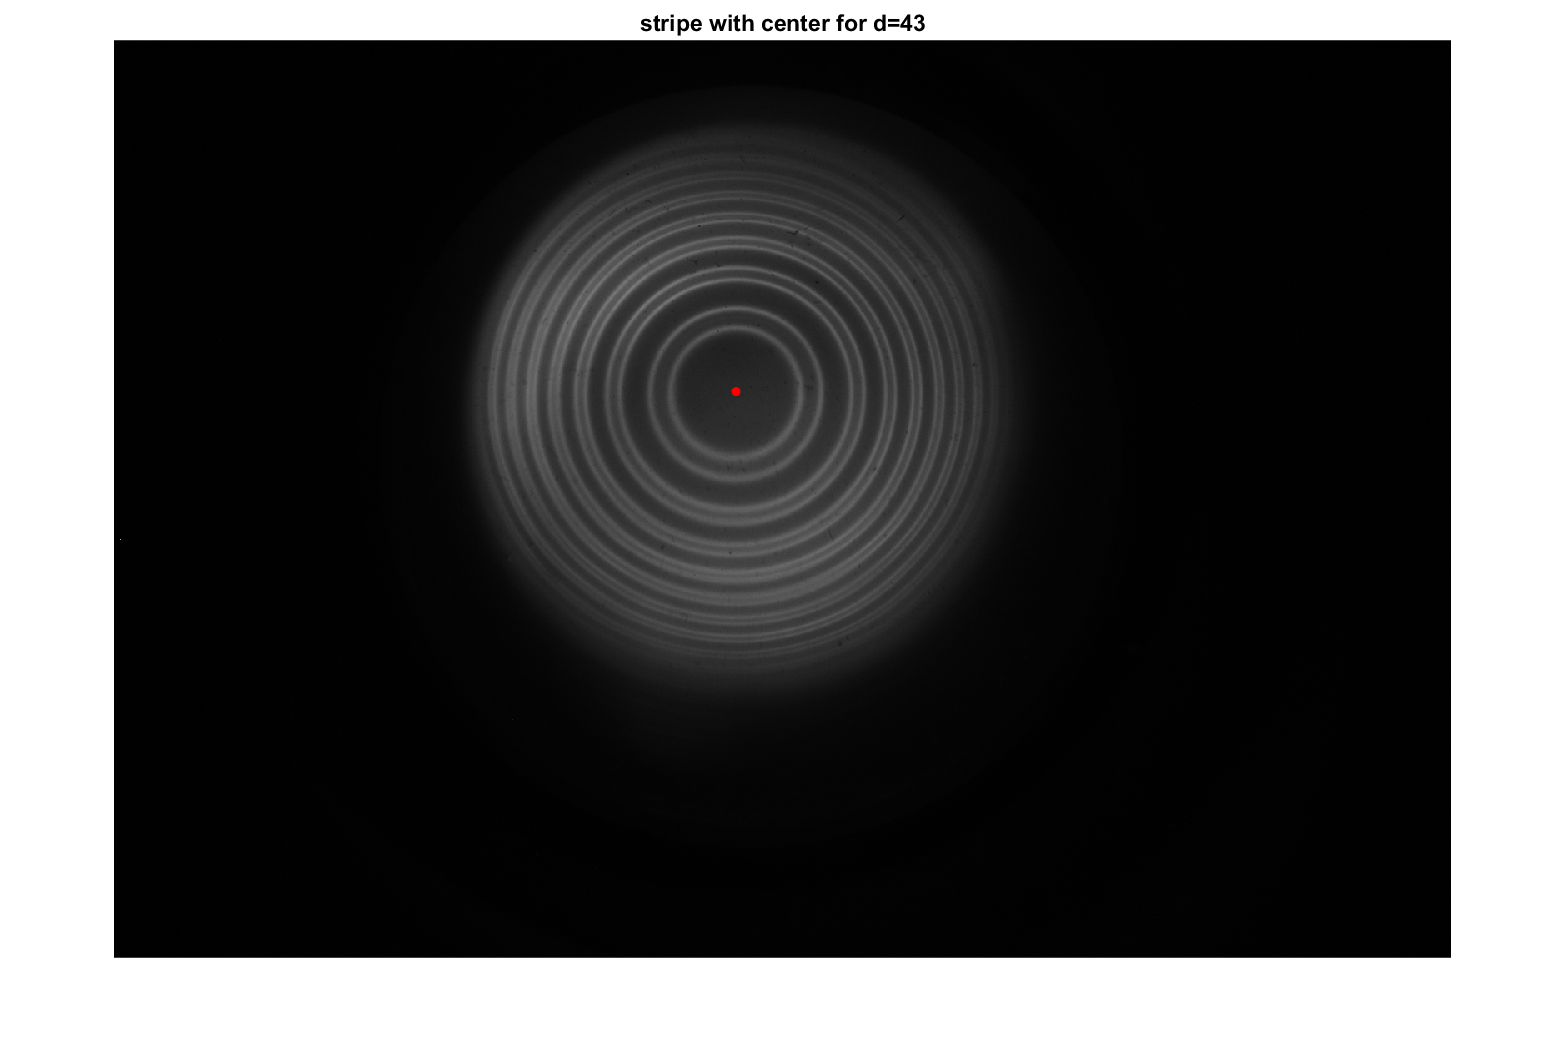
\includegraphics[width=\textwidth]{stripe_with_center_43.png}
            \caption{Stripes with center.}
            \label{fig:stripe with center}
    \end{figure}
    
    \par Secondly we extract the data of the horizontal and vertical lines passing through the center of the circle . And we use Fourier analysis to remove the high frequency noise (about f = 500) and then transform it back, resulting in smoother data (Fig.\ref{fig:horizontal intensity} shows the horizontal part).
    
    \begin{figure}[H]
        \centering
        \begin{subfigure}[b]{0.48\textwidth}
            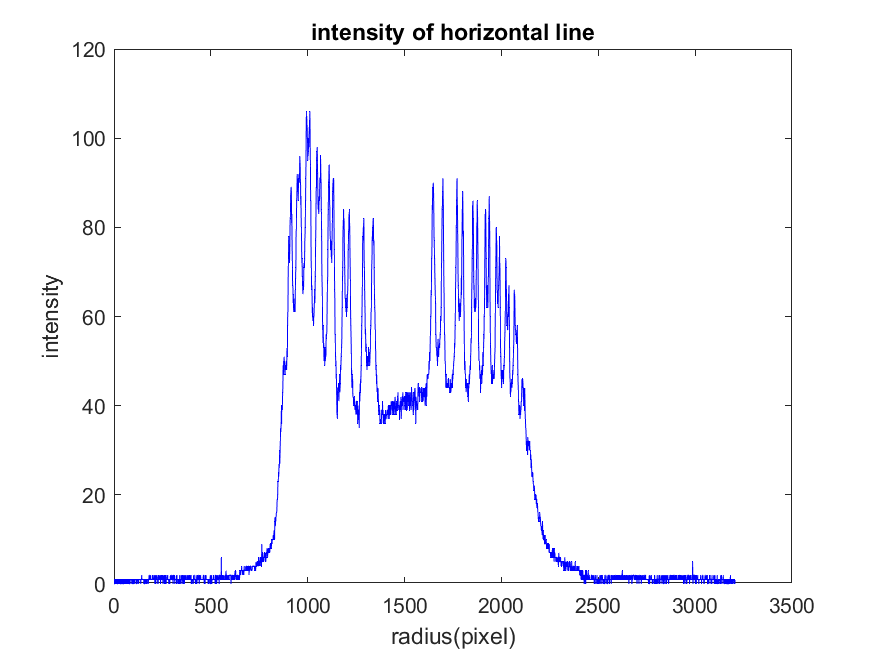
\includegraphics[width=\textwidth]{horizontal_intensity_43.png}
            \caption{Horizontal intensity of the stripes.}
        \end{subfigure}
        \begin{subfigure}[b]{0.48\textwidth}
            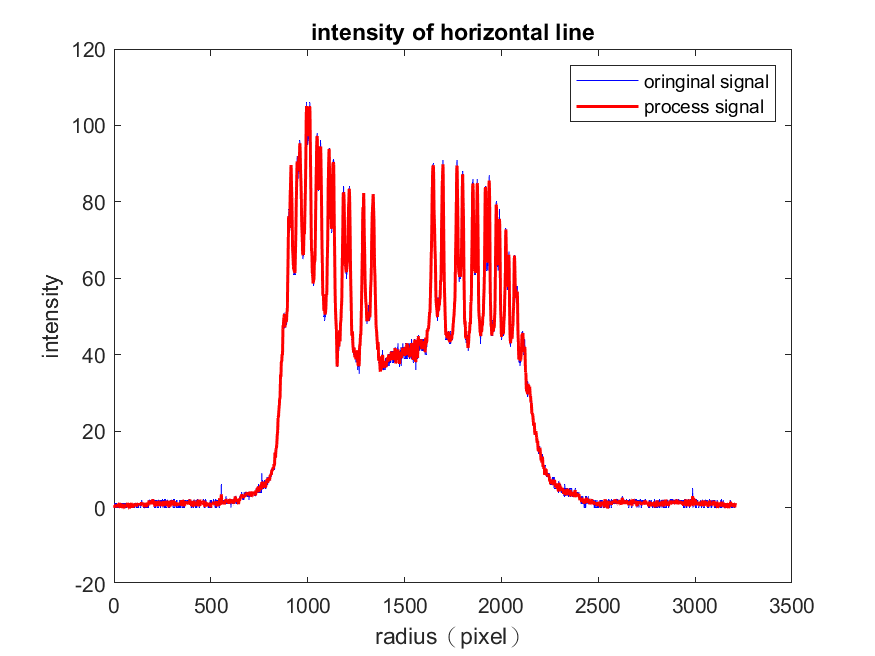
\includegraphics[width=\textwidth]{horizontal_intensity__processed_43.png}
            \caption{Horizontal intensity of the stripes with processed signal.}
        \end{subfigure}
        \caption{Horizontal intensity of transverse normal Zeeman effect.}
        \label{fig:horizontal intensity}
    \end{figure}
    
    
    \par Finally we can calculate the radius of every circle. Subsequently, all data will be extracted using these five fixed points d = 43, 45, 48, 50, 53 mm (Fig.\ref{fig:tra_nor_fiveimages}), we calculate the radius after we extract the signal from four directions, and take the average, Tab.\ref{tab:tra_nor} shows the data. And we will do the uncertainty at the same time, it comes from the combination of the resolution of the image and the standard deviation of data of four directions. The former contributes $\frac{1}{2\sqrt{3}} $ (pixel) and the latter contributes $\frac{\text{stand deviation}}{\sqrt{\text{number}}} $ (pixel), shown in Tab.\ref{tab:tra_nor_un}.
    
    \begin{figure}[H]
      \centering
      
      \begin{subfigure}[b]{0.3\textwidth}
        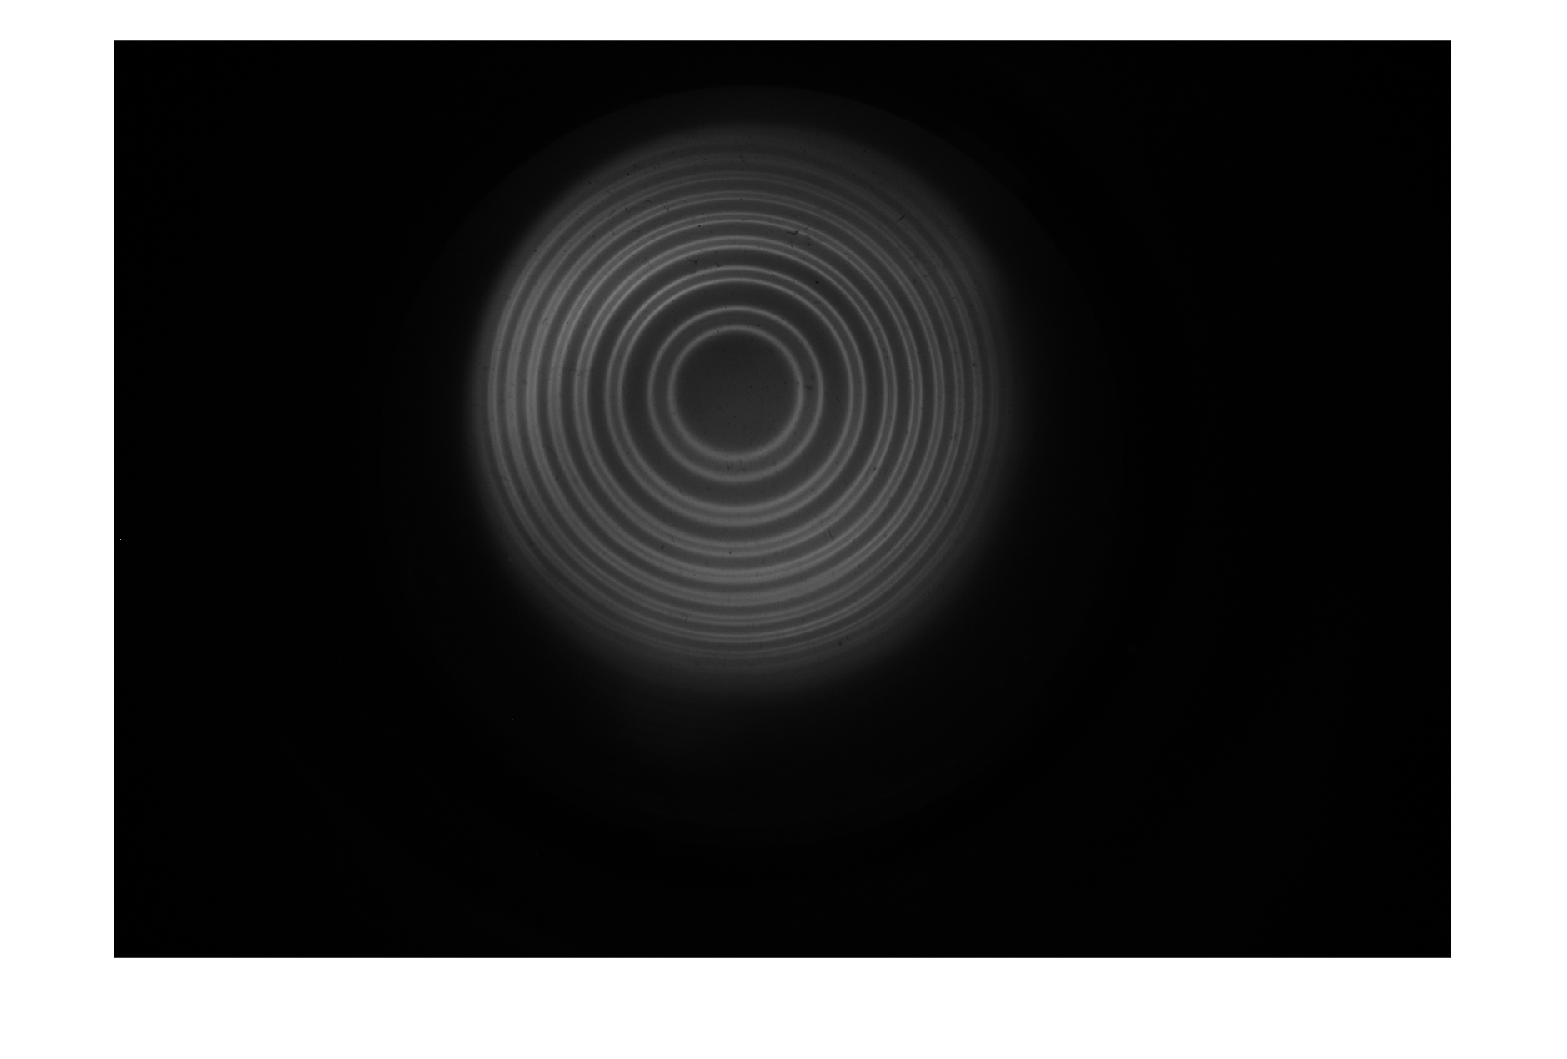
\includegraphics[width=1.2\textwidth]{tra_nor_stripe_43.png}
        \caption{43mm}
      \end{subfigure}
      \hfill
      \begin{subfigure}[b]{0.3\textwidth}
        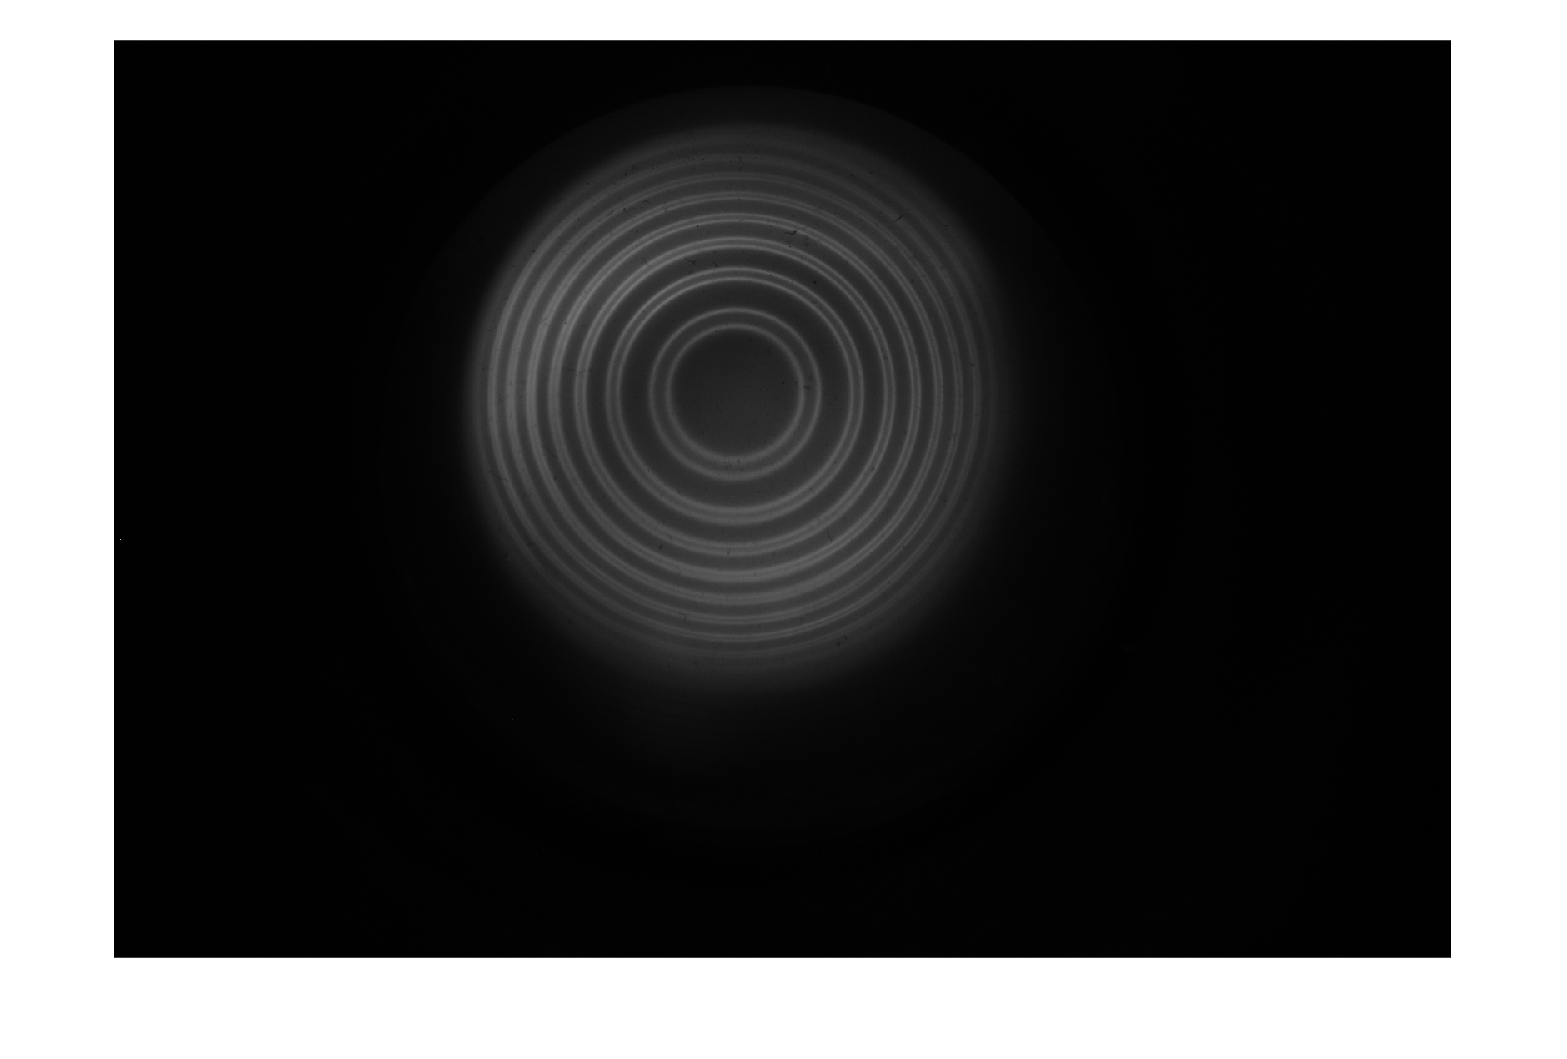
\includegraphics[width=1.2\textwidth]{tra_nor_stripe_45.png}
        \caption{45mm}
      \end{subfigure}
      \hfill
      \begin{subfigure}[b]{0.3\textwidth}
        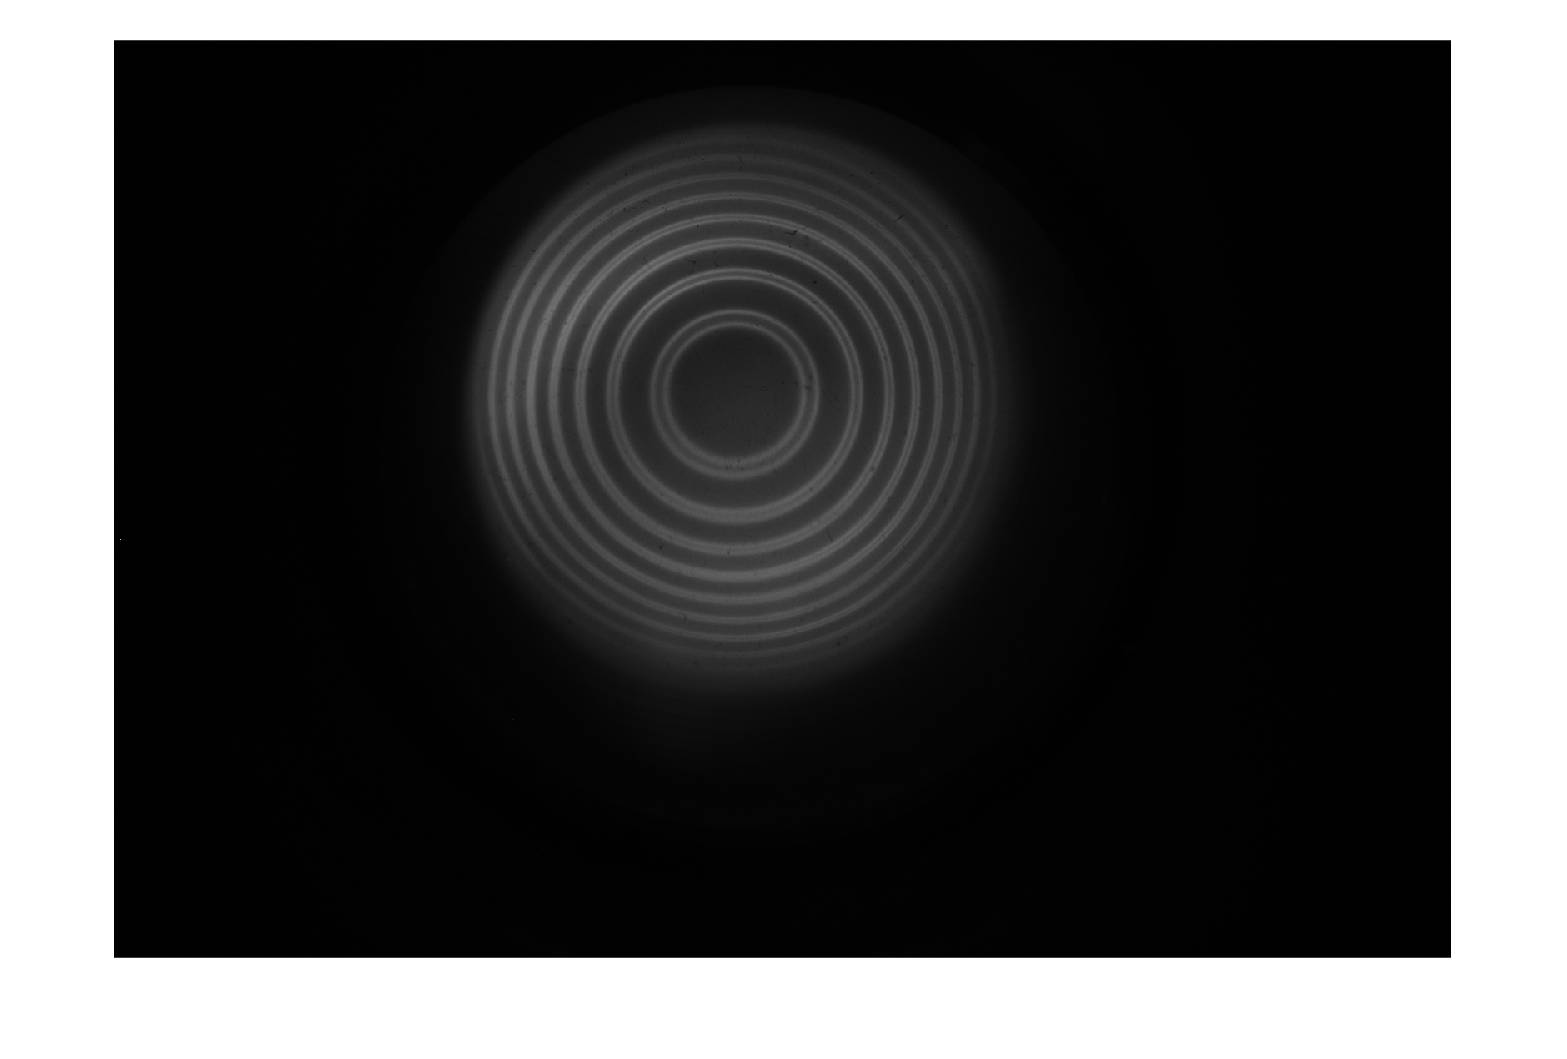
\includegraphics[width=1.2\textwidth]{tra_nor_stripe_48.png}
        \caption{48mm}
      \end{subfigure}
    
      \vspace{0.5cm}
    
      \begin{subfigure}[b]{0.3\textwidth}
        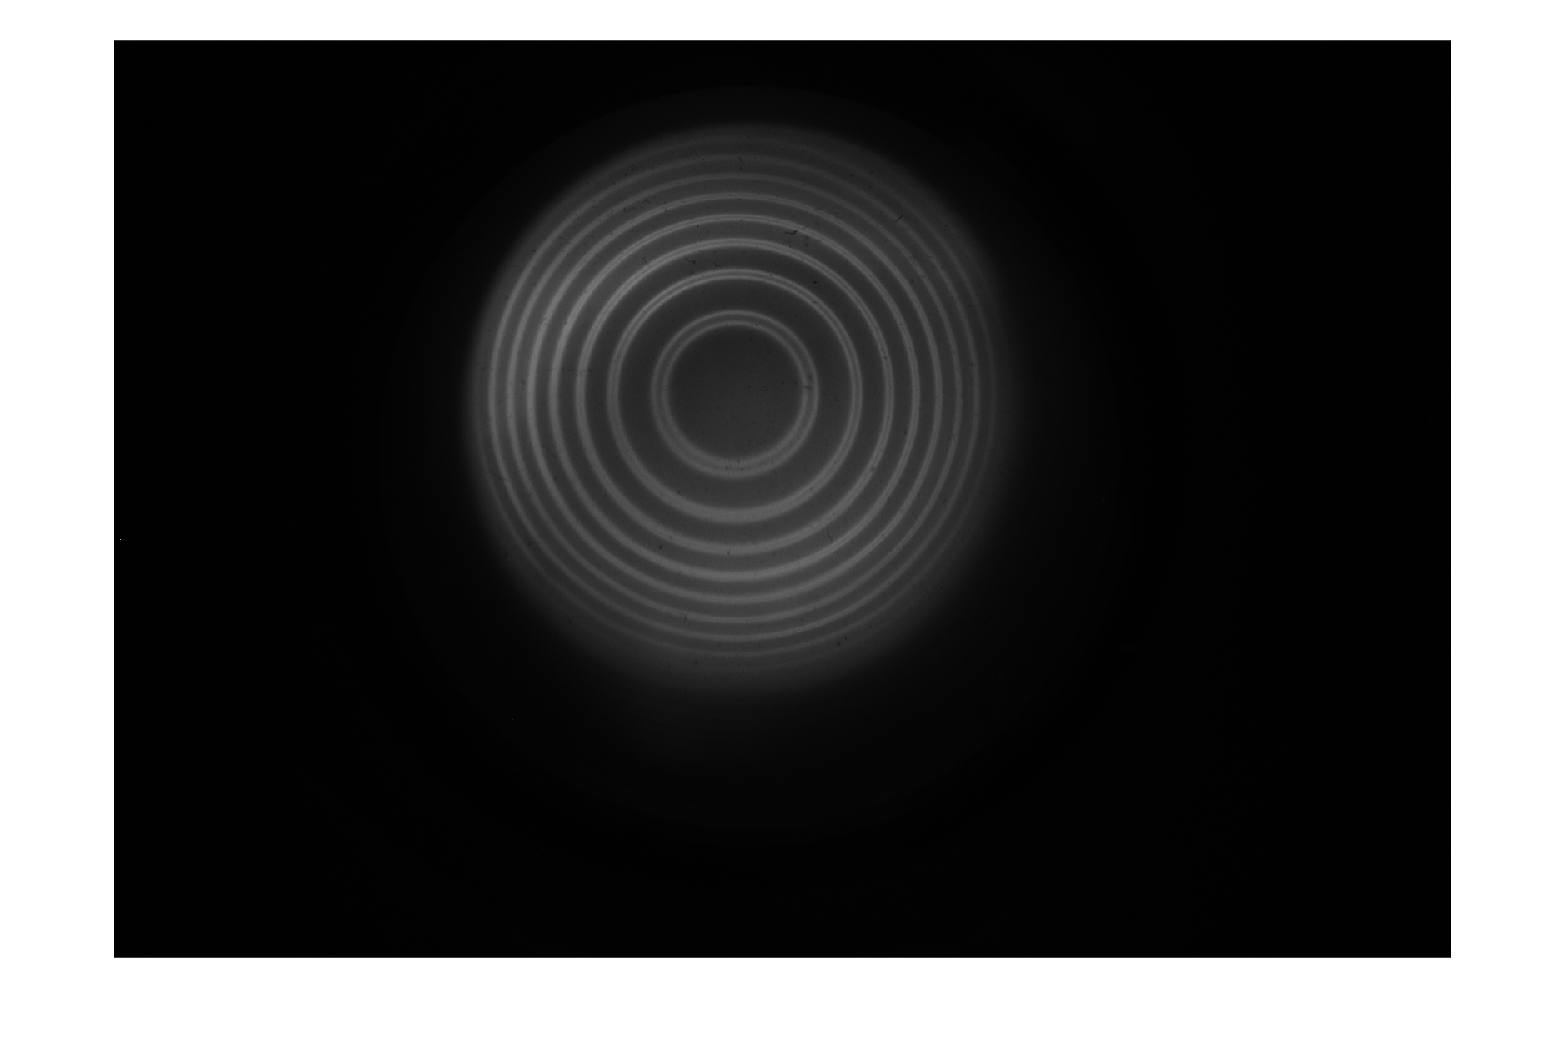
\includegraphics[width=1.2\textwidth]{tra_nor_stripe_50.png}
        \caption{50mm}
      \end{subfigure}
      \hfill
      \begin{subfigure}[b]{0.3\textwidth}
        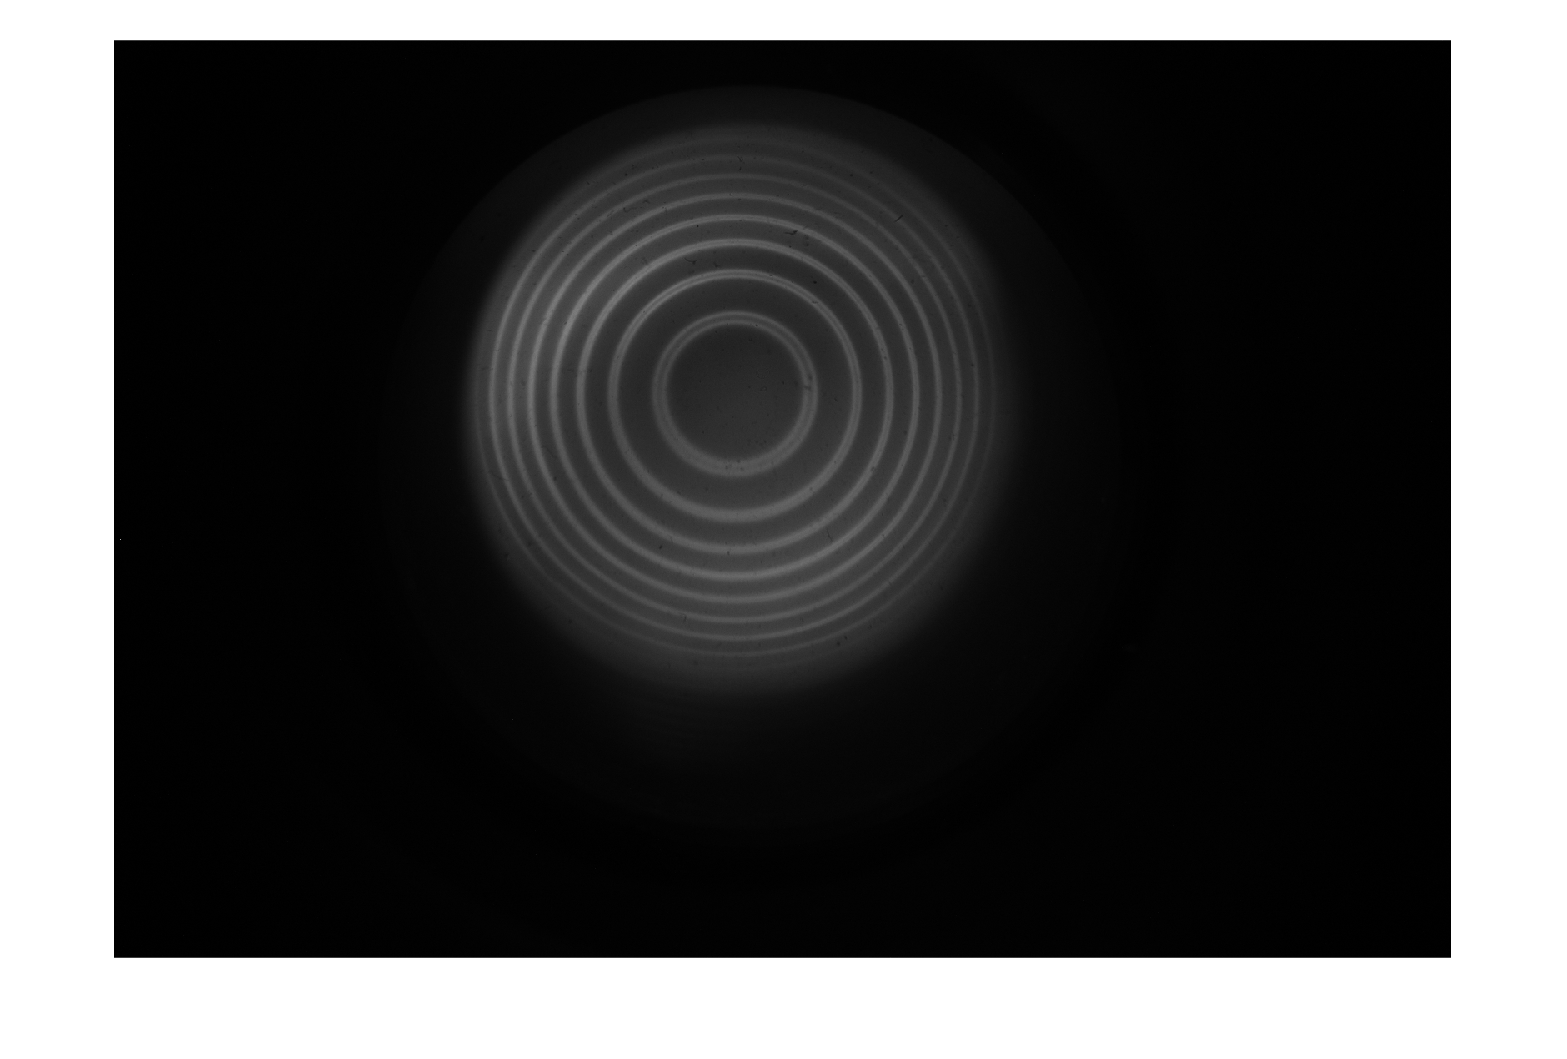
\includegraphics[width=1.2\textwidth]{tra_nor_stripe_53.png}
        \caption{53mm}
      \end{subfigure}
    
      \caption{Observation of transverse normal Zeeman effect.}
      \label{fig:tra_nor_fiveimages}
    \end{figure}
    
    \begin{table}[H]
        \centering
        \caption{Radius of transversal normal Zeeman effect.}
        \begin{tabular}{c|c|c|c|c|c|c}
            $d $ (mm)& $C1 $ (pixel)& $C2 $ (pixel)& $C3 $ (pixel)& $C4 $ (pixel)& $C5 $ (pixel)& $C6 $ (pixel)\\ \hline \hline
            43&	155   &	179.25 & 205   & 276.75& 292.75&306.25 \\ \hline
            45&	160.25&	181.25 & 199.5 & 279.75& 292.75&303.75 \\ \hline
            48&	165.5 &	181.75 & 195.25& 282.75& 292   &301.5 \\ \hline
            50&	166.5 &	180.5  & 193.25& 284   & 292   &297.5 \\ \hline
            53&	171.5 &	182	   & 192   & 285   & 291   & 295.75 \\ \hline
        \end{tabular}
        \label{tab:tra_nor}
    \end{table}
    
    \begin{table}[H]
        \centering
        \caption{Uncertainties of radius of transversal normal Zeeman effect.}
        \begin{tabular}{c|c|c|c|c|c|c}
            $d $ (mm)& $u_{C1} $ (pixel)& $u_{C2} $ (pixel)& $u_{C3} $ (pixel)& $u_{C4} $ (pixel)& $u_{C5} $ (pixel)& $u_{C6} $ (pixel) \\ \hline \hline
            43&1.6583&2.0766&2.6925&3.1589&4.1205&3.937  \\ \hline
            45&1.7736&2.5124&2.3452&3.6486&4.3565&3.6486 \\ \hline
            48&1.8708&3.1589&1.726 &3.5794&4.213 &4.062  \\ \hline
            50&2.5495&4.2229&2.5779&4.3874&4.8904&3.8078 \\ \hline
            53&2.972 &2.6925&3.0413&4.0311&3.5   &3.8051 \\ \hline
        \end{tabular}
        \label{tab:tra_nor_un}
    \end{table}
    
    \par And we calculate the area of every circle, the differences of the splitting stripes areas and the differences of energy level areas, then take the average, thus we have $\delta_{1}$ and $\delta_{2}$ which is the average of the difference of splitting stripe area from two different energy levels, and $\Delta$ is the average of the difference between the energy levels. And the uncertainties are the results of the error propagation, in which it experience the calculation of area, subtraction, average, and finally the division of $\delta$ and $\Delta$ , we won't be elaborating it's equations. The result is shown in Table.\ref{tab:tra_nor_side} and Tab.\ref{tab:tra_nor_final}.
    
    \begin{table}[H]
        \centering
        \caption{Side product before the final result, where $\delta_{1}$ is the average of 1 and 2 cells, $\delta_{2}$ is the average of 3 and 4 cells, and $\Delta$ is the average of 5 and 6 and 7 cells.Units are all square of pixel }
        \resizebox{\textwidth}{!}{%
        \begin{tabular}{c|c|c|c|c|c|c|c|c|c|c}
            $d $ (mm)& C2-C1& C3-C2& C5-C4& C6-C5& C4-C1& C5-C2&C6-C3&$\delta_{1}$&$\delta_{2}$&$\Delta$ \\ \hline \hline
            43&25464.37&31084.29&28626.19&25404.48&165139.58&168301.40&162621.59&28274.33&27015.34&165354.19  \\ \hline
            45&22529.93&21829.94&23381.30&20613.56&165184.94&166036.31&164819.92&22179.93&21997.43&165347.06 \\ \hline
            48&17727.41&15989.13&16702.08&17713.08&165113.66&164088.32&165812.27&16858.27&17207.58&165004.75  \\ \hline
            50&15261.85&14970.67&14476.45&10185.82&166296.28&165510.88&160726.04&15116.26&12331.14&164177.734 \\ \hline
            53&11660.80&11749.55&10857.34&8755.81&162774.55&161971.09&158977.35&11705.18&9806.57&161240.99 \\ \hline
        \end{tabular}
        \label{tab:tra_nor_side}
    }
    \end{table}
    
    \begin{table}[H]
        \centering
        \caption{Final result of transversal normal Zeeman effect.}
        \begin{tabular}{c|c|c|c|c|c|c}
            $d $ (mm)& $B $ (T)& $\frac{\delta_{1}}{\Delta}$ & $\frac{\delta_{2}}{\Delta}$& $u_{B} $ (T)& $u_{\frac{\delta_{1}}{\Delta}} $& $u_{\frac{\delta_{2}}{\Delta}} $ \\ \hline \hline
            43&0.29435&0.17099&0.16337&0.0063519&0.015921&0.043232  \\ \hline
            45&0.23958&0.13414&0.13303&0.0030616&0.016451&0.044792 \\ \hline
            48&0.19281&0.10216&0.10428&0.0011630&0.017961&0.044947  \\ \hline
            50&0.1274&0.092072&0.075108&0.0044667&0.024299&0.050371 \\ \hline        53&0.08443&0.072594&0.060819&0.0019575&0.020356&0.042097 \\ \hline
        \end{tabular}
        \label{tab:tra_nor_final}
    \end{table}
    
    \par And we can find the relation between $\frac{\delta_{1}}{\Delta}$, $\frac{\delta_{2}}{\Delta}$ and the magnetic field by looking for the fitting line, which is shown in Fig.\ref{fig:tra_nor_data}.
    
    \begin{figure}[H]
        \centering
        \begin{subfigure}[b]{0.48\textwidth}
            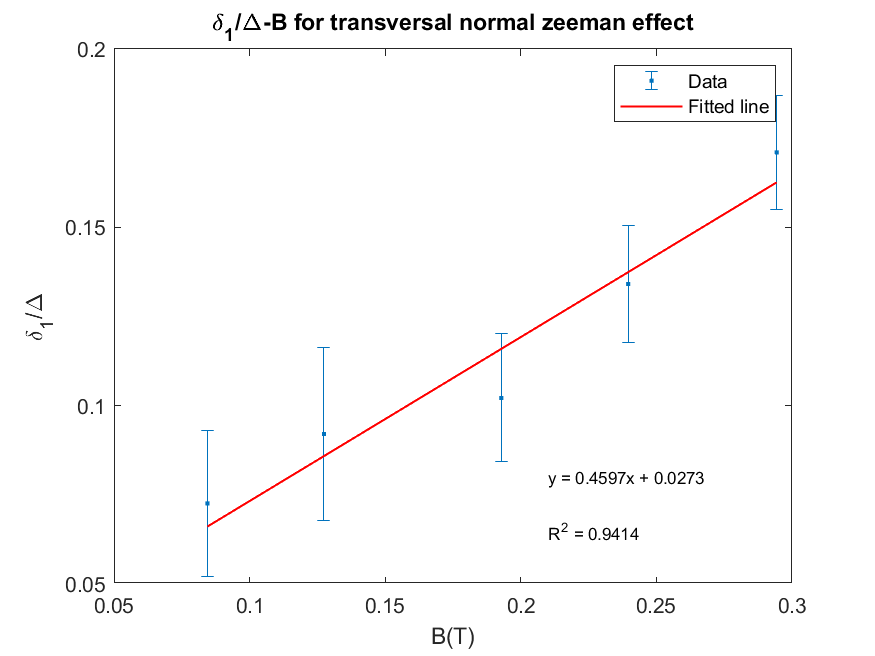
\includegraphics[width=\textwidth]{tra_nor_d1_data.png}
            \caption{Fitting line for $\frac{\delta_{1}}{\Delta}$ with B.}
        \end{subfigure}
        \begin{subfigure}[b]{0.48\textwidth}
            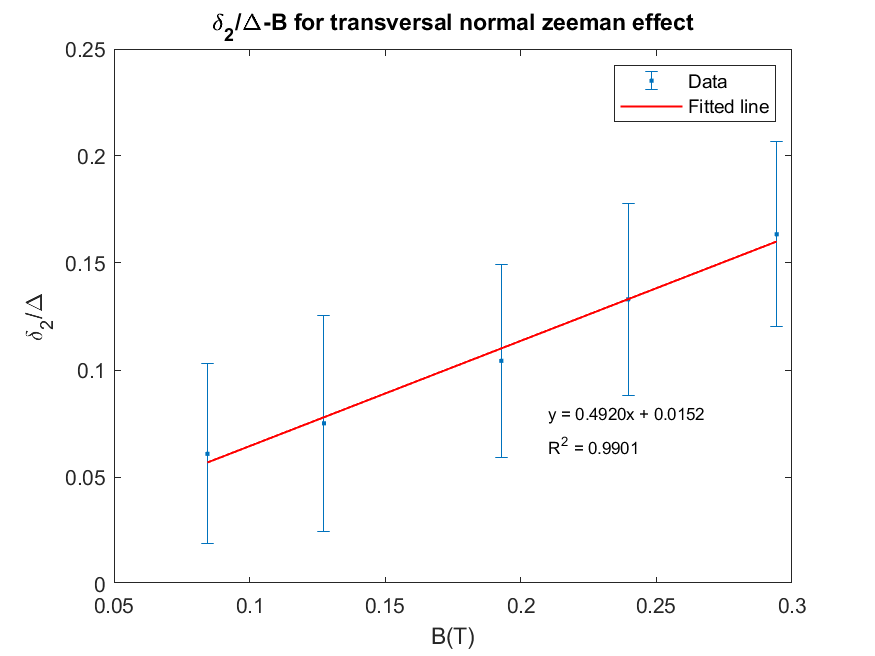
\includegraphics[width=\textwidth]{tra_nor_d2_data.png}
            \caption{Fitting line for $\frac{\delta_{2}}{\Delta}$ with B.}
        \end{subfigure}
        \caption{Fitting line of transversal normal Zeeman effect.}
        \label{fig:tra_nor_data}
    \end{figure}
    
    \par We use weighted least squares method to find the fitting line and the uncertainty of the slope, once we have that for both two fitting lines, we can take its average and calculate Bohr magneton using Eq.\ref{eq:bohr mag}, where $\mu$ = 1.452 and $t$ = 0.003 (m) is given by the lecture, and the uncertainty is the error propagation of Eq.\ref{eq:bohr mag}, with the existing error from the slope. The theoretical value is $9.273\cdot 10^{-24}$ (J/T), and the  result is shown in Tab.\ref{tab:tra_nor_final_data}. 
    
    \begin{equation}
        \mu_B = \frac{hc}{2\mu t} \cdot \frac{\delta}{\Delta B}=\frac{hc}{2\mu t} \cdot \text{slope}
        \label{eq:bohr mag}  
    \end{equation}
    
    \begin{table}[H]
        \centering
        \caption{Data of transversal normal Zeeman effect.}
        \begin{tabular}{c|c|c|c|c|c}
             &slope1 (1/T)& slope2 (1/T)& average slope (1/T)& $\mu_B$ (1/T)& diff \% \\ \hline \hline
            value&0.45972&0.49021&0.474965&$1.08299\cdot 10^{-23}$&0.1679  \\ \hline
            uncertainty&0.11435&0.26056&0.284547&$6.48814\cdot10^{-24}$& \\ \hline
            
        \end{tabular}
        \label{tab:tra_nor_final_data}
    \end{table}
    
    \subsubsection{Transversal Anomalous Zeeman Effect (Vertical)}\label{4.2.3}
    
    \par In this and the next sector in which we discuss in vertical polarization, the steps are the same as the last sector thus we only shows the observation and the data. 
    
    \begin{figure}[H]
      \centering
      
      \begin{subfigure}[b]{0.3\textwidth}
        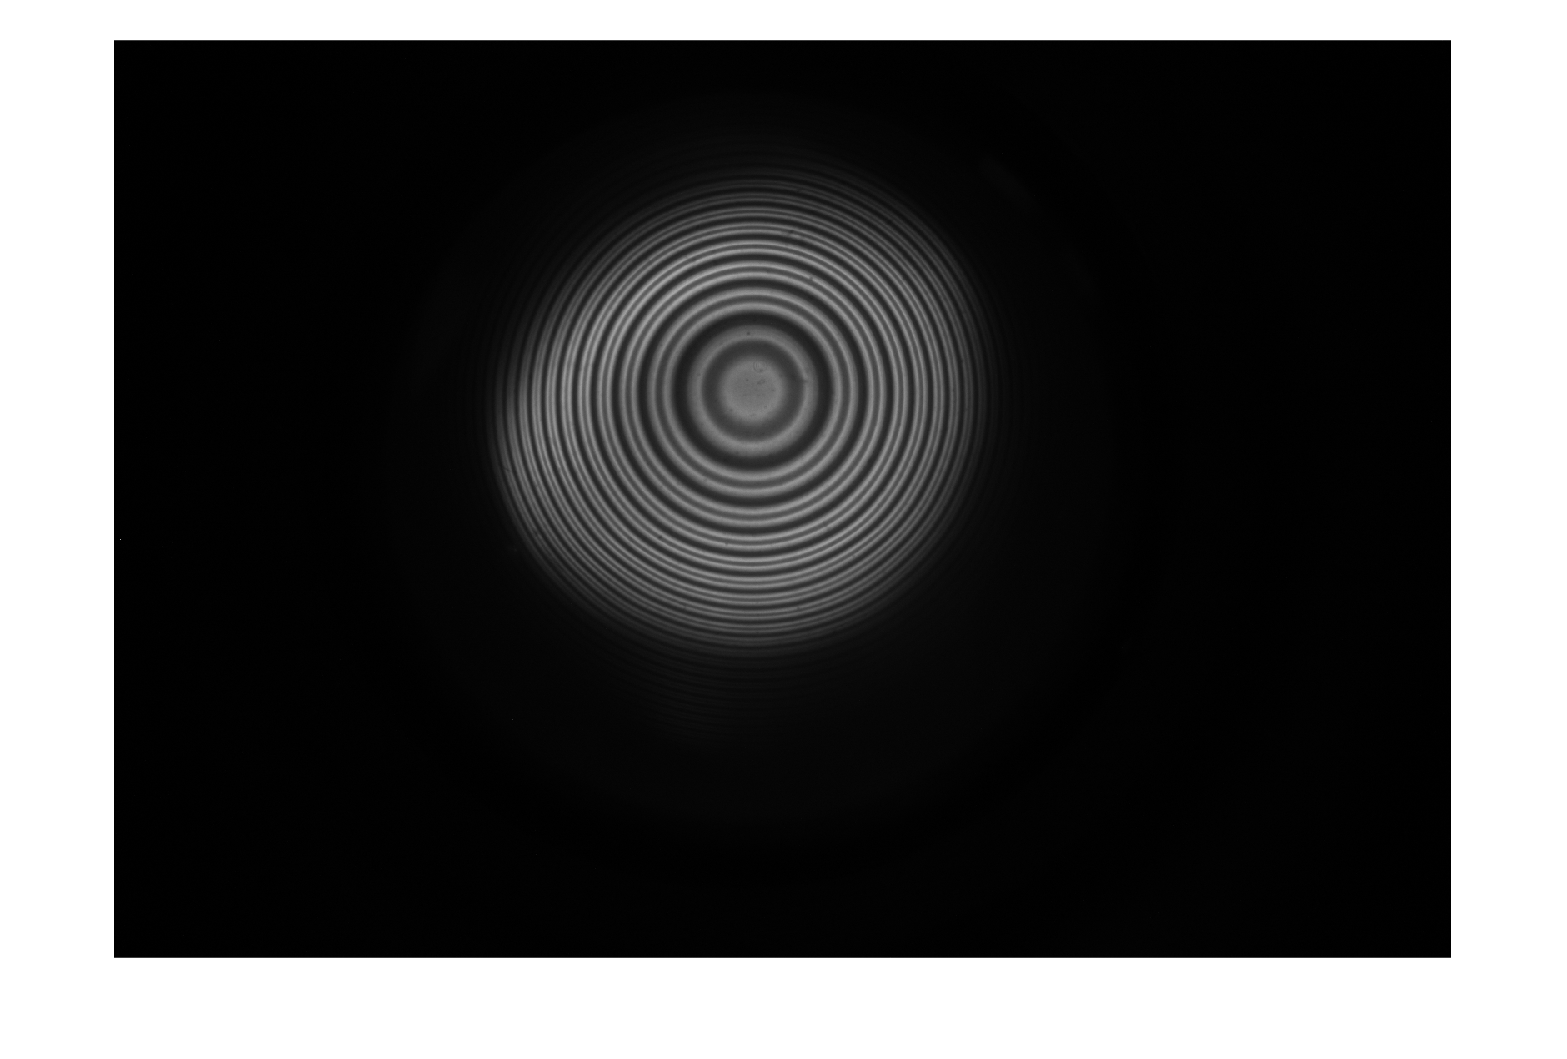
\includegraphics[width=1.2\textwidth]{tra_ano_stripe_ver_43.png}
        \caption{43mm}
      \end{subfigure}
      \hfill
      \begin{subfigure}[b]{0.3\textwidth}
        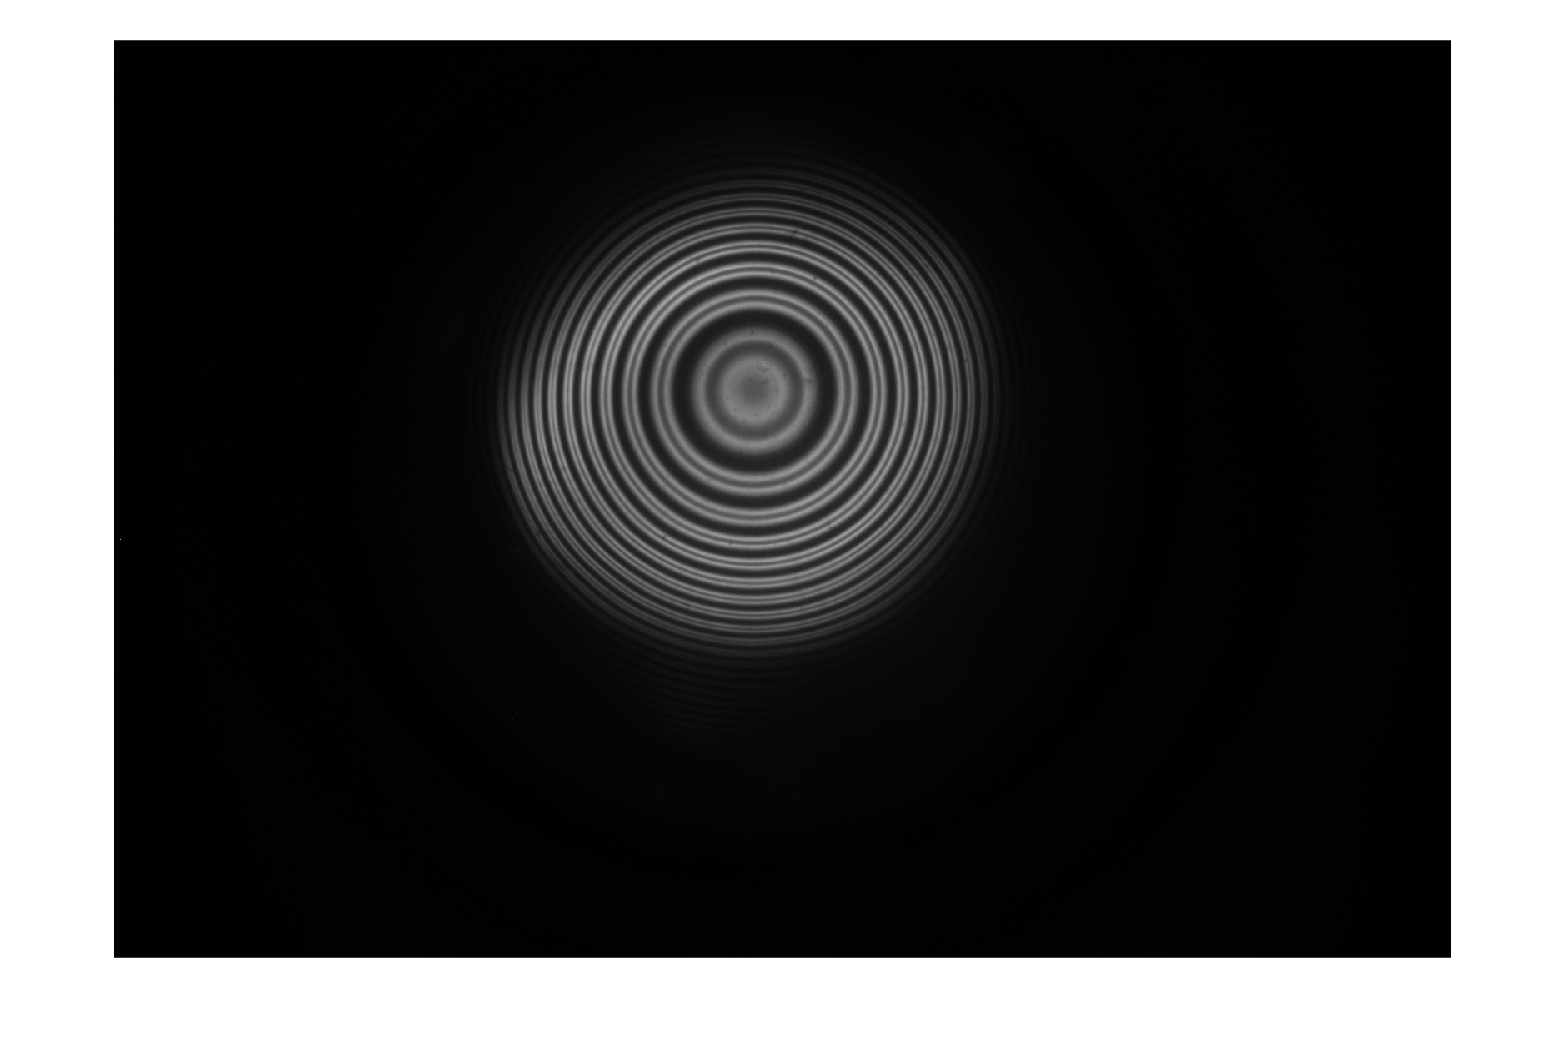
\includegraphics[width=1.2\textwidth]{tra_ano_stripe_ver_45.png}
        \caption{45mm}
      \end{subfigure}
      \hfill
      \begin{subfigure}[b]{0.3\textwidth}
        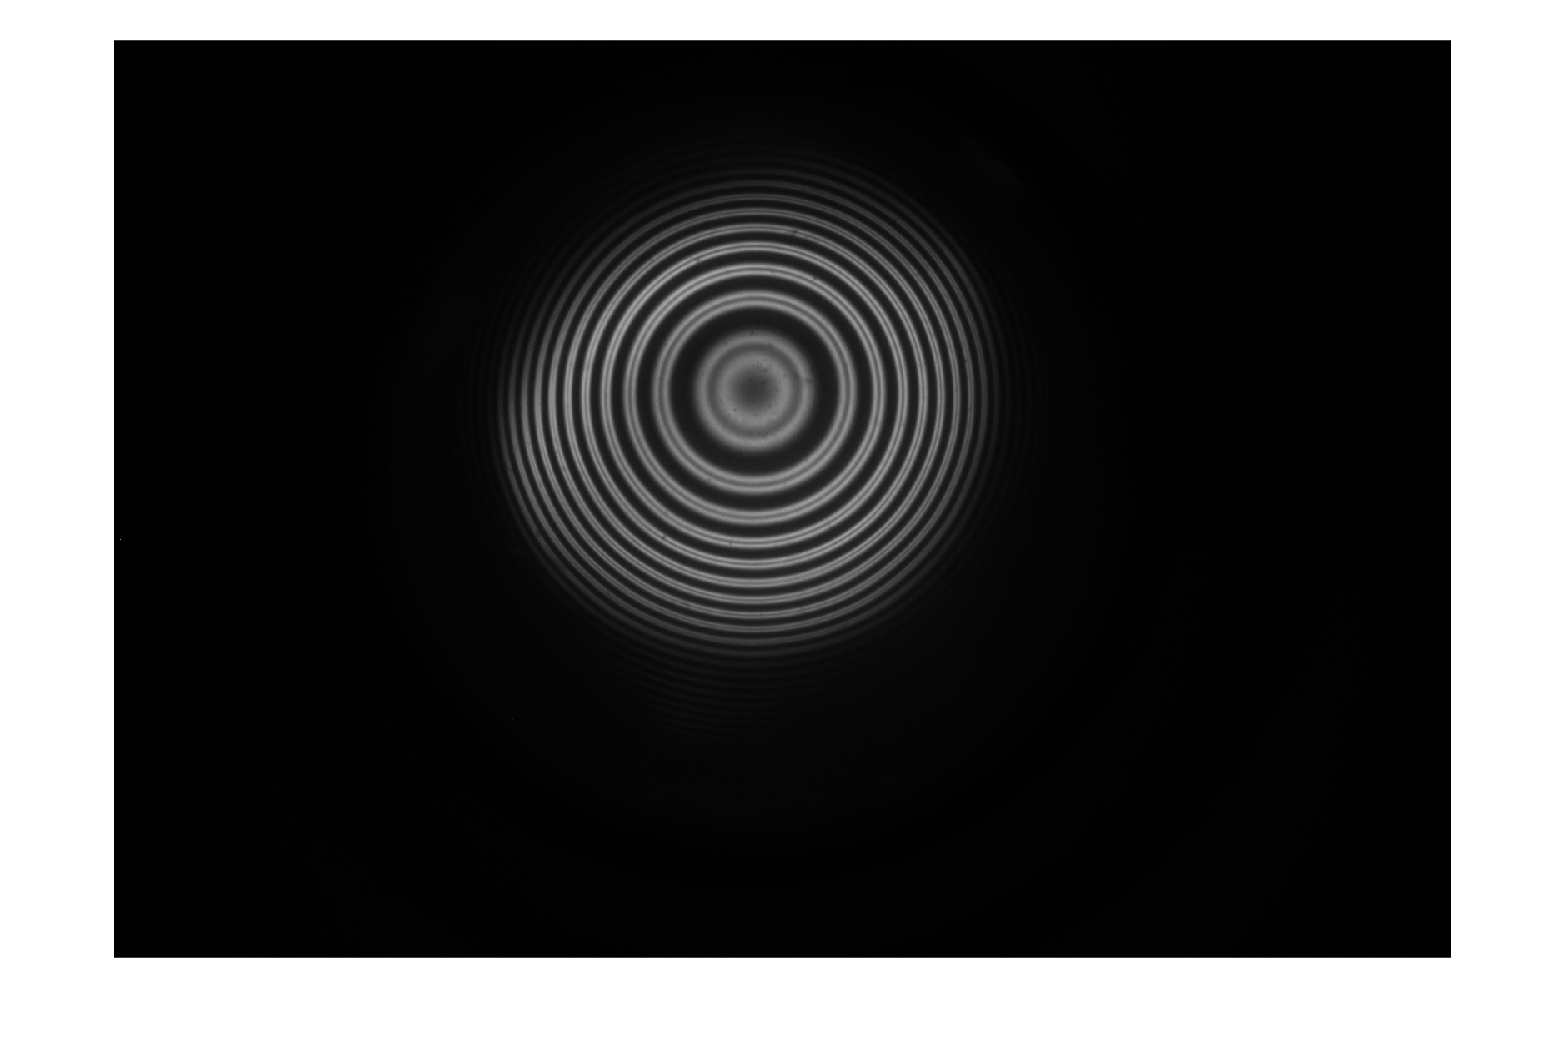
\includegraphics[width=1.2\textwidth]{tra_ano_stripe_ver_48.png}
        \caption{48mm}
      \end{subfigure}
    
      \vspace{0.5cm}
    
      \begin{subfigure}[b]{0.3\textwidth}
        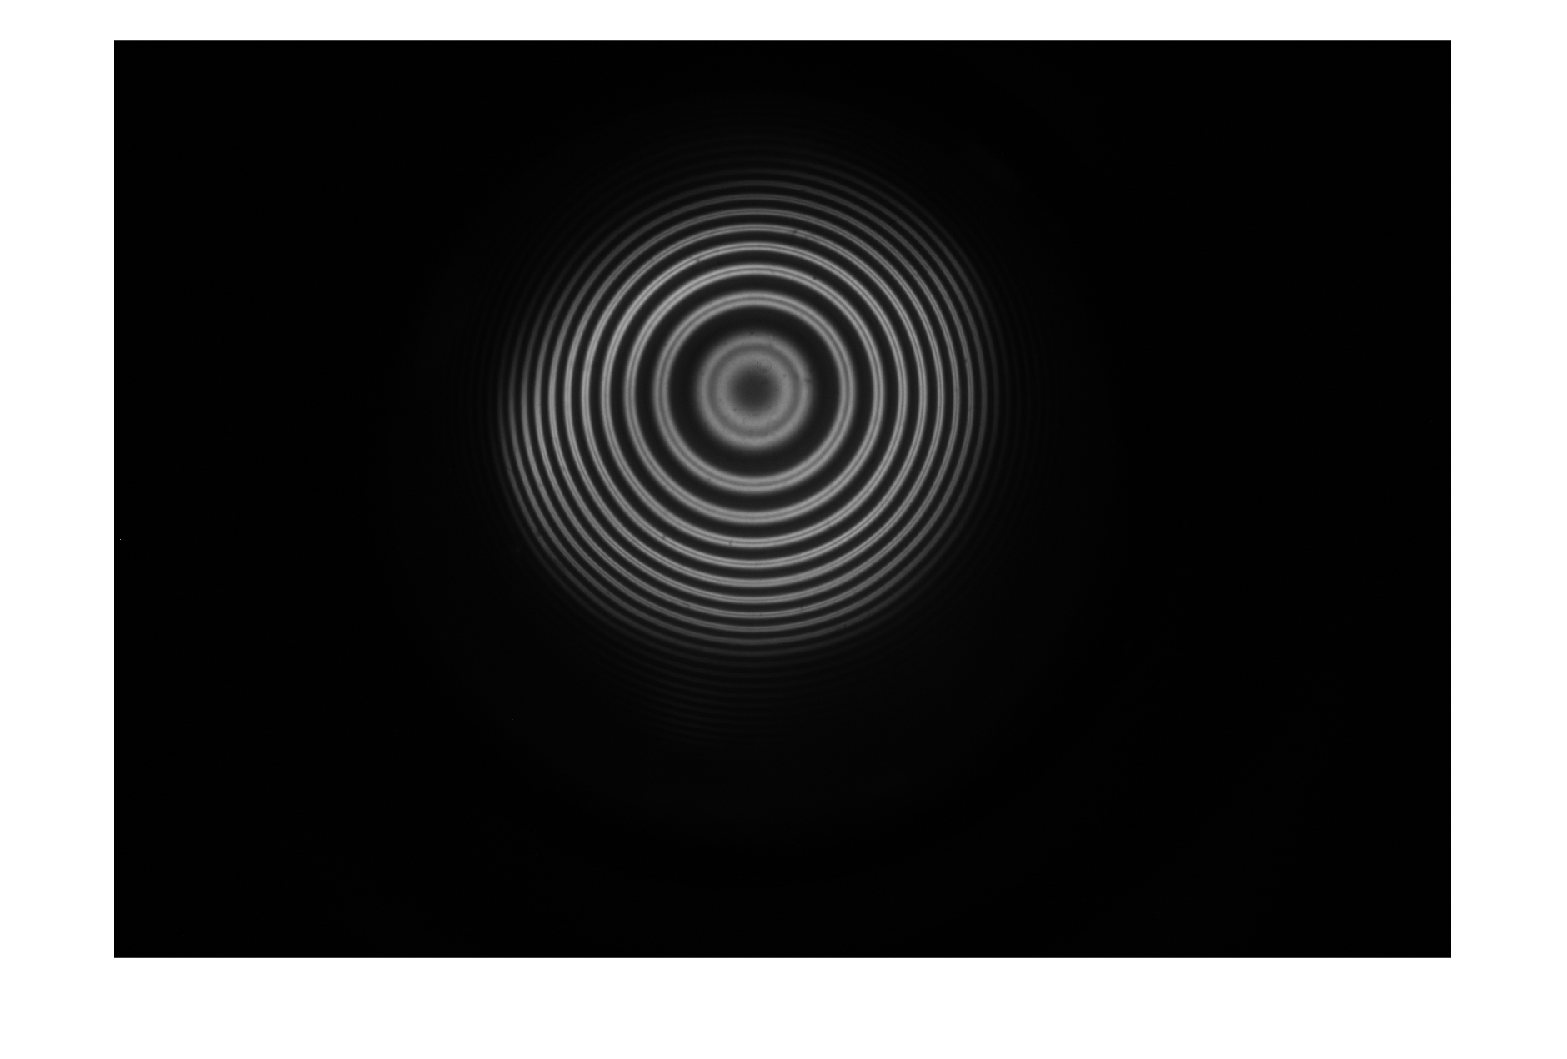
\includegraphics[width=1.2\textwidth]{tra_ano_stripe_ver_50.png}
        \caption{50mm}
      \end{subfigure}
      \hfill
      \begin{subfigure}[b]{0.3\textwidth}
        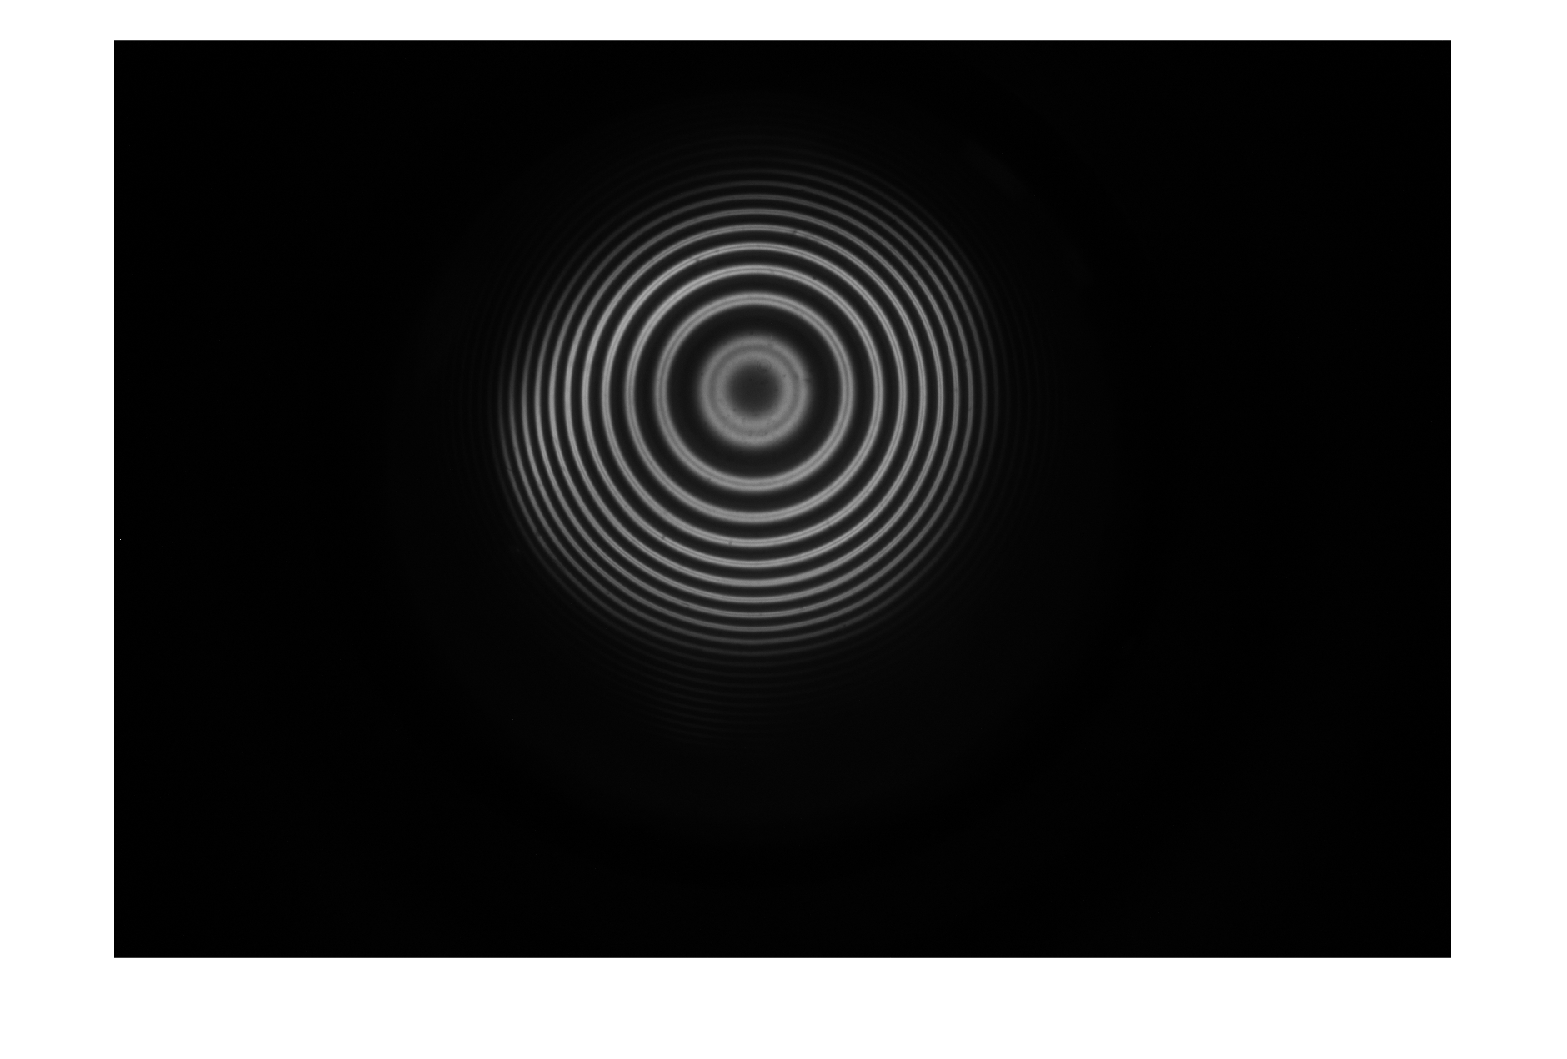
\includegraphics[width=1.2\textwidth]{tra_ano_stripe_ver_53.png}
        \caption{53mm}
      \end{subfigure}
    
      \caption{Observation of transverse anomalous Zeeman effect (Vertical).}
      \label{fig:tra_ano_ver_fiveimages}
    \end{figure}
    
    \begin{table}[H]
        \centering
        \caption{Radius of transversal anomalous Zeeman effect (Vertical).}
        \begin{tabular}{c|c|c|c|c}
            $d $ (mm)& $C1 $ (pixel)& $C2 $ (pixel)& $C3 $ (pixel)& $C4 $ (pixel) \\ \hline \hline
            43&	208.5	&237.5	&286	&309.25 \\ \hline
            45&	210.25	&236.25	&288.5	&307.75 \\ \hline
            48&	213.25	&234	&290.75	&305.75 \\ \hline
            50&	214.25	&233	&292	&305 \\ \hline
            53&	217.75	&230.75	&293.75	&303.25 \\ \hline
        \end{tabular}
        \label{tab:tra_ano_ver}
    \end{table}
    
    \begin{table}[H]
        \centering
        \caption{Uncertainties of radius of transversal anomalous Zeeman effect (Vertical).}
        \begin{tabular}{c|c|c|c|c}
            $d $ (mm)& $u_{C1} $ (pixel)& $u_{C2} $ (pixel)& $u_{C3} $ (pixel)& $u_{C4} $ (pixel)  \\ \hline \hline
            43&2.1015&2.3979&3.9370&4.6075  \\ \hline
            45&2.7195&2.8099&3.7080&4.3660 \\ \hline
            48&2.6575&2.6457&4.1508&4.3084  \\ \hline
            50&2.6575&2.7386&4.3397&4.1633 \\ \hline
            53&2.3935&2.6887&4.3660&4.1306 \\ \hline
        \end{tabular}
        \label{tab:tra_ano_ver_un}
    \end{table}
    
    \begin{table}[H]
        \centering
        \caption{Side product before the final result, where $\delta$ is the average of 1 and 2 cells, and $\Delta$ is the average of 3 and 4 cells. Units are all square of pixel }
        \resizebox{\textwidth}{!}{%
        \begin{tabular}{c|c|c|c|c|c|c}
            $d $ (mm)& C2-C1& C4-C3& C3-C1& C4-C2&$\delta$&$\Delta$ \\ \hline \hline
            43&40633.35&43478.26&120397.61&123242.52&42055.81&121820.06   \\ \hline
            45&36470.74&36058.61&122607.52&122195.38&36264.68&122401.45 \\ \hline
            48&29155.35&28109.40&122710.60&121664.65&28632.37&122187.63  \\ \hline
            50&26345.19&24381.90&123656.03&121692.73&25363.55&122674.38 \\ \hline
            53&18317.05&17817.54&122126.27&121626.75&18067.29&121876.51 \\ \hline
        \end{tabular}
        \label{tab:tra_ano_side}
    }
    \end{table}
    
    \begin{table}[H]
        \centering
        \caption{Final result of transversal anomalous Zeeman effect (Vertical).}
        \begin{tabular}{c|c|c|c|c}
            $d $ (mm)& $B $ (T)& $\frac{\delta}{\Delta}$ & $u_{B} $ (T)& $u_{\frac{\delta}{\Delta}} $ \\ \hline \hline
            43&0.29435&0.34522&0.0063519&0.053284  \\ \hline
            45&0.23958&0.29627&0.0030616&0.051612 \\ \hline
            48&0.19281&0.23433&0.0011630&0.052125  \\ \hline
            50&0.1274 &0.20675&0.0044667&0.051971 \\ \hline        
            53&0.08443&0.14824&0.0019575&0.051266 \\ \hline
        \end{tabular}
        \label{tab:tra_ano_final}
    \end{table}
    
    \begin{figure}[H]
        \centering
        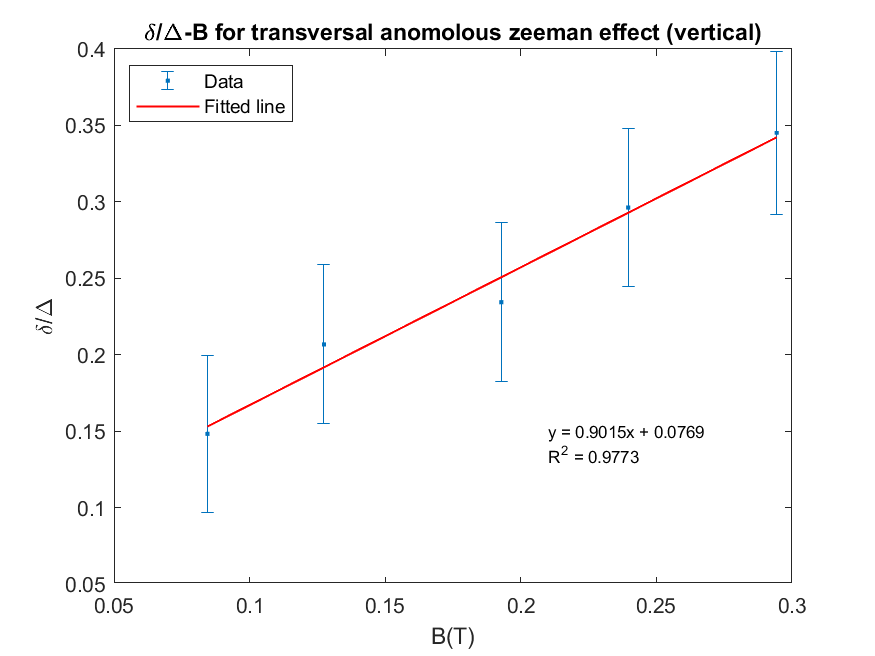
\includegraphics[width=0.8\textwidth]{tra_ano_ver_data.png}
            \caption{Fitting line of transversal anomalous Zeeman effect (Horizontal).}
        \label{fig:tra_ano_ver_data}
    \end{figure}
    
    \par The Bohr magneton for this situation is given by Eq.\ref{eq:bohr mag_2}, where $\mu$ = 1.452 and $t$ = 0.003 (m).
    
    \begin{equation}
        \mu_B = \frac{hc}{3\mu t} \cdot \frac{\delta}{\Delta B}=\frac{hc}{3\mu t} \cdot \text{slope}
        \label{eq:bohr mag_2}  
    \end{equation}
    
    \begin{table}[H]
        \centering
        \caption{Data of transversal anomalous Zeeman effect (Vertical).}
        \begin{tabular}{c|c|c|c}
             &slope (1/T)& $\mu_B$ (1/T)& diff \% \\ \hline \hline
            value&0.90148&$1.37034\cdot 10^{-23}$&0.4777  \\ \hline
            uncertainty&0.31084&$4.72509\cdot 10^{-24}$& \\ \hline
            
        \end{tabular}
        \label{tab:tra_ano_ver_final_data}
    \end{table}
    
    \subsubsection{Transversal Anomalous Zeeman Effect (Horizontal)}\label{4.2.4}
    
    \begin{figure}[H]
      \centering
      
      \begin{subfigure}[b]{0.3\textwidth}
        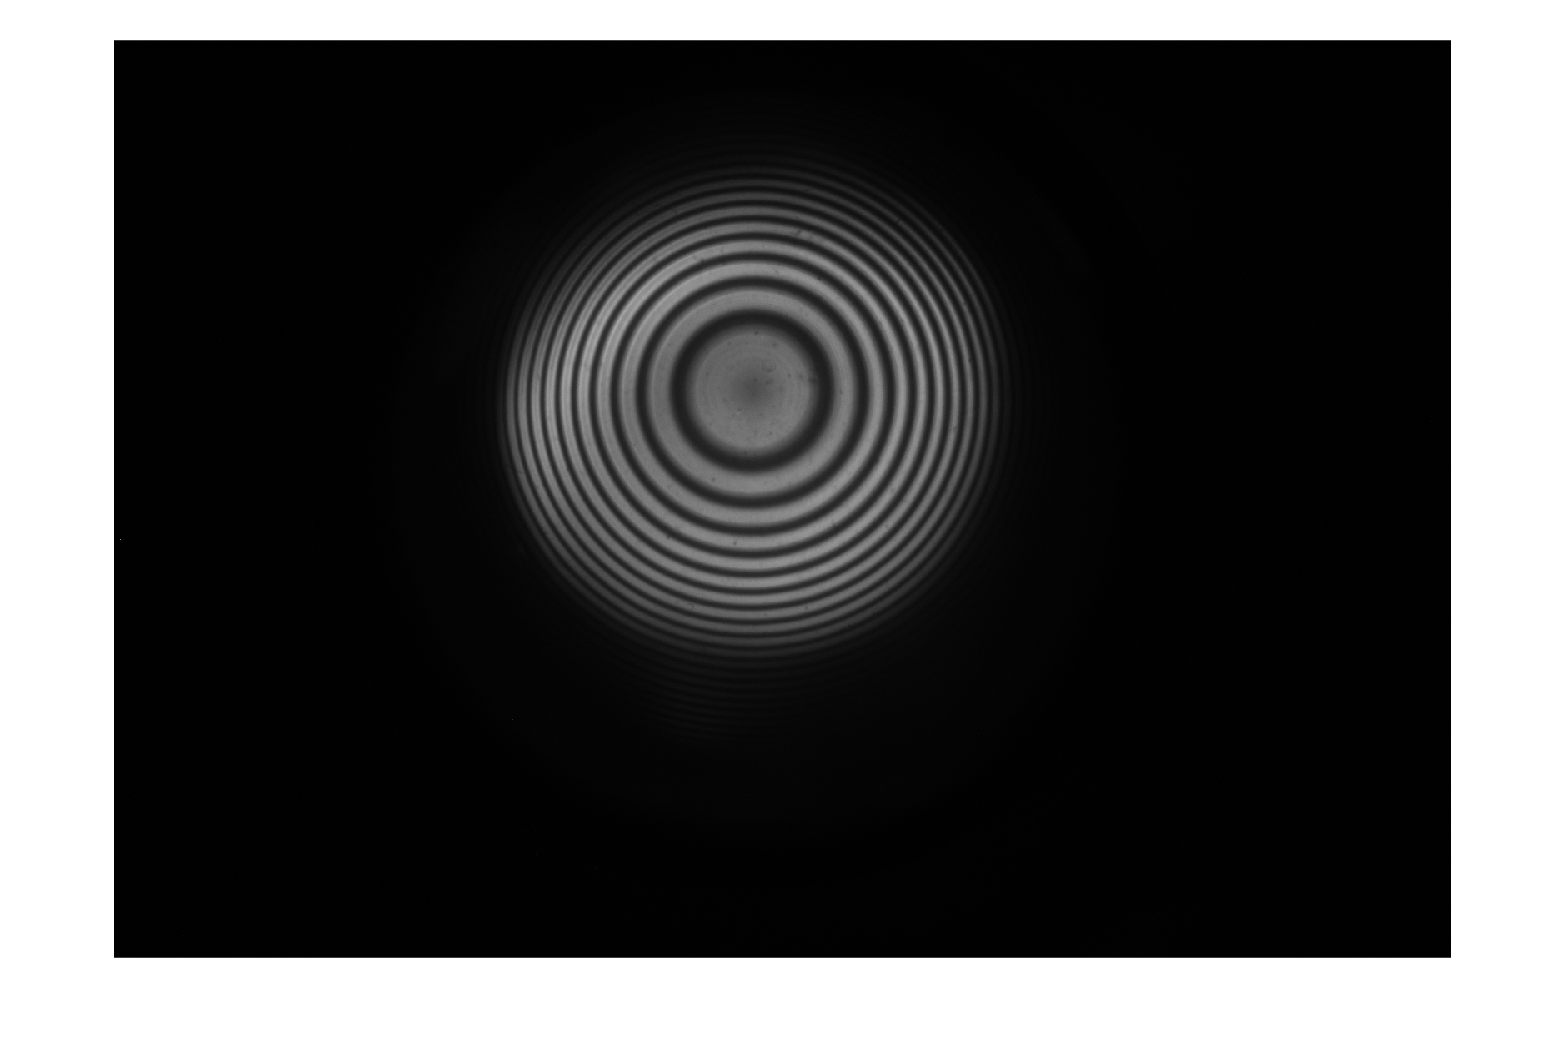
\includegraphics[width=1.2\textwidth]{tra_ano_stripe_hor_43.png}
        \caption{43mm}
      \end{subfigure}
      \hfill
      \begin{subfigure}[b]{0.3\textwidth}
        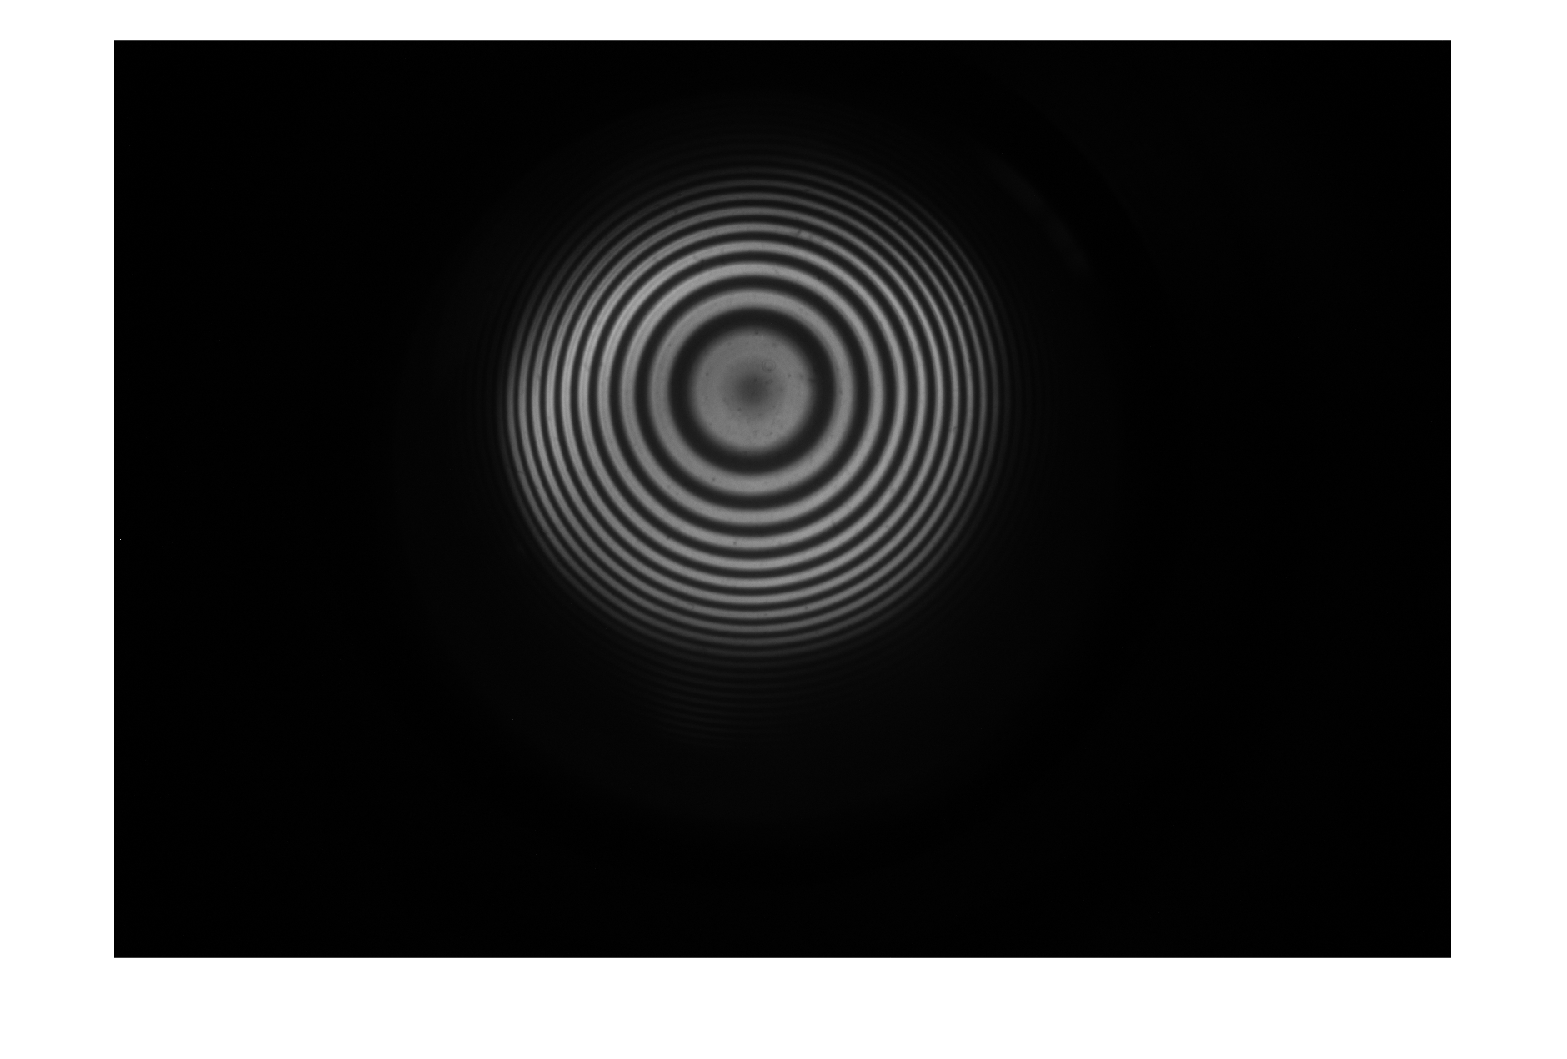
\includegraphics[width=1.2\textwidth]{tra_ano_stripe_hor_45.png}
        \caption{45mm}
      \end{subfigure}
      \hfill
      \begin{subfigure}[b]{0.3\textwidth}
        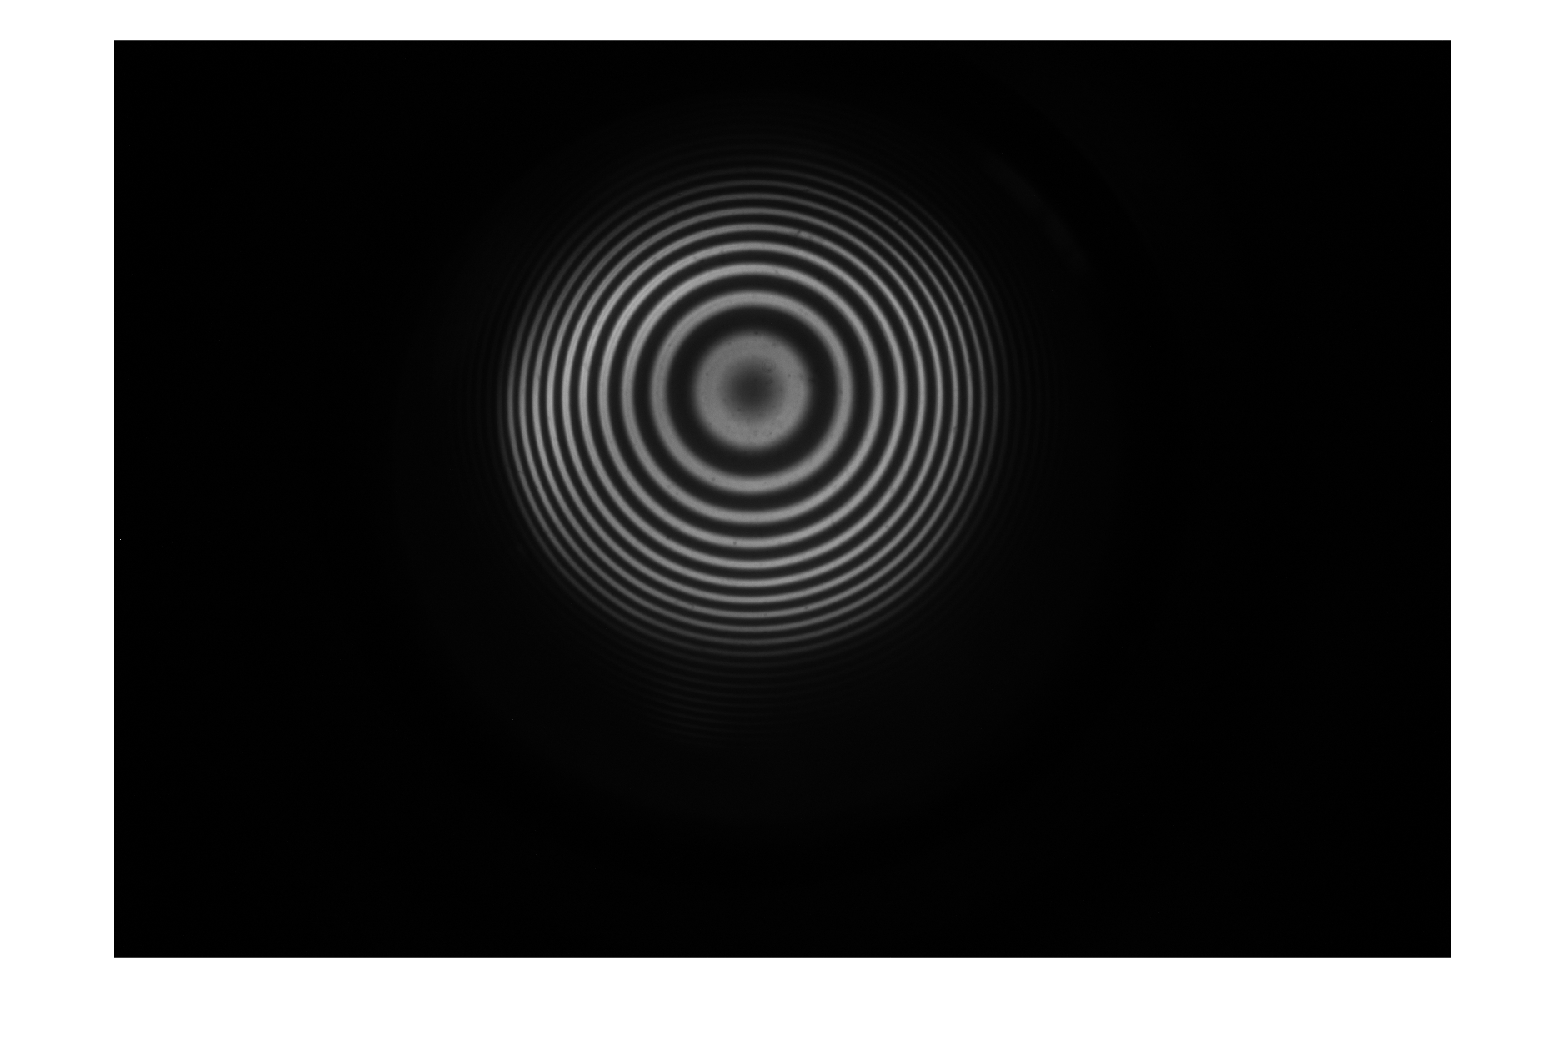
\includegraphics[width=1.2\textwidth]{tra_ano_stripe_hor_48.png}
        \caption{48mm}
      \end{subfigure}
    
      \vspace{0.5cm}
    
      \begin{subfigure}[b]{0.3\textwidth}
        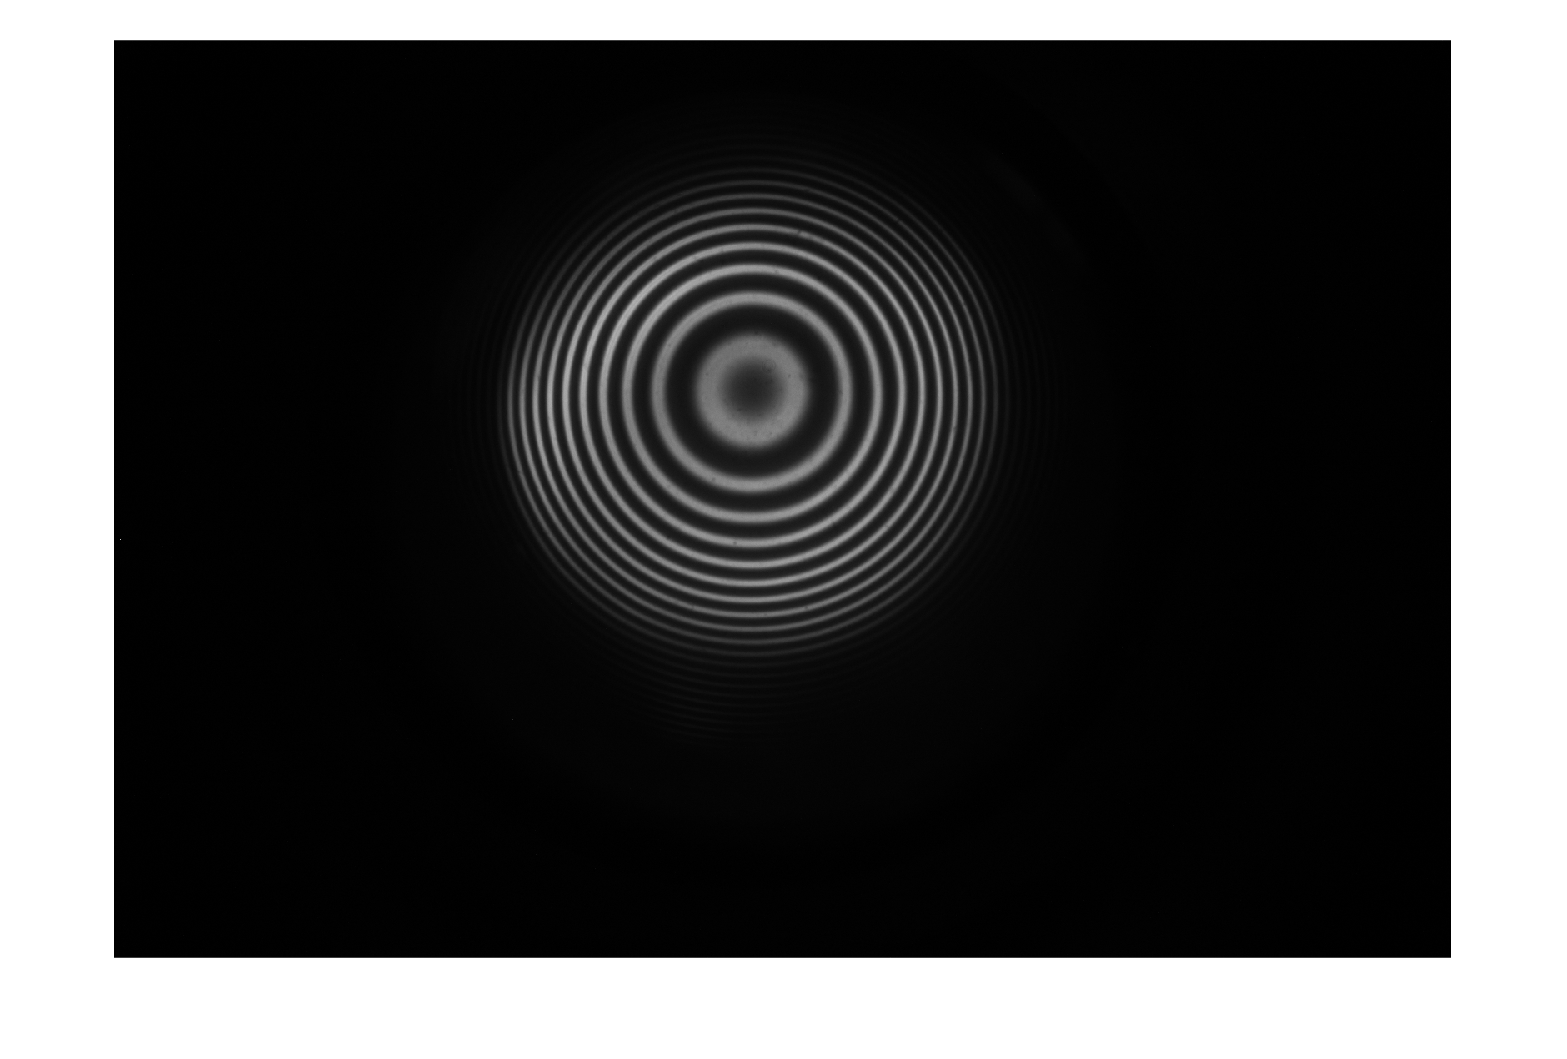
\includegraphics[width=1.2\textwidth]{tra_ano_stripe_hor_50.png}
        \caption{50mm}
      \end{subfigure}
      \hfill
      \begin{subfigure}[b]{0.3\textwidth}
        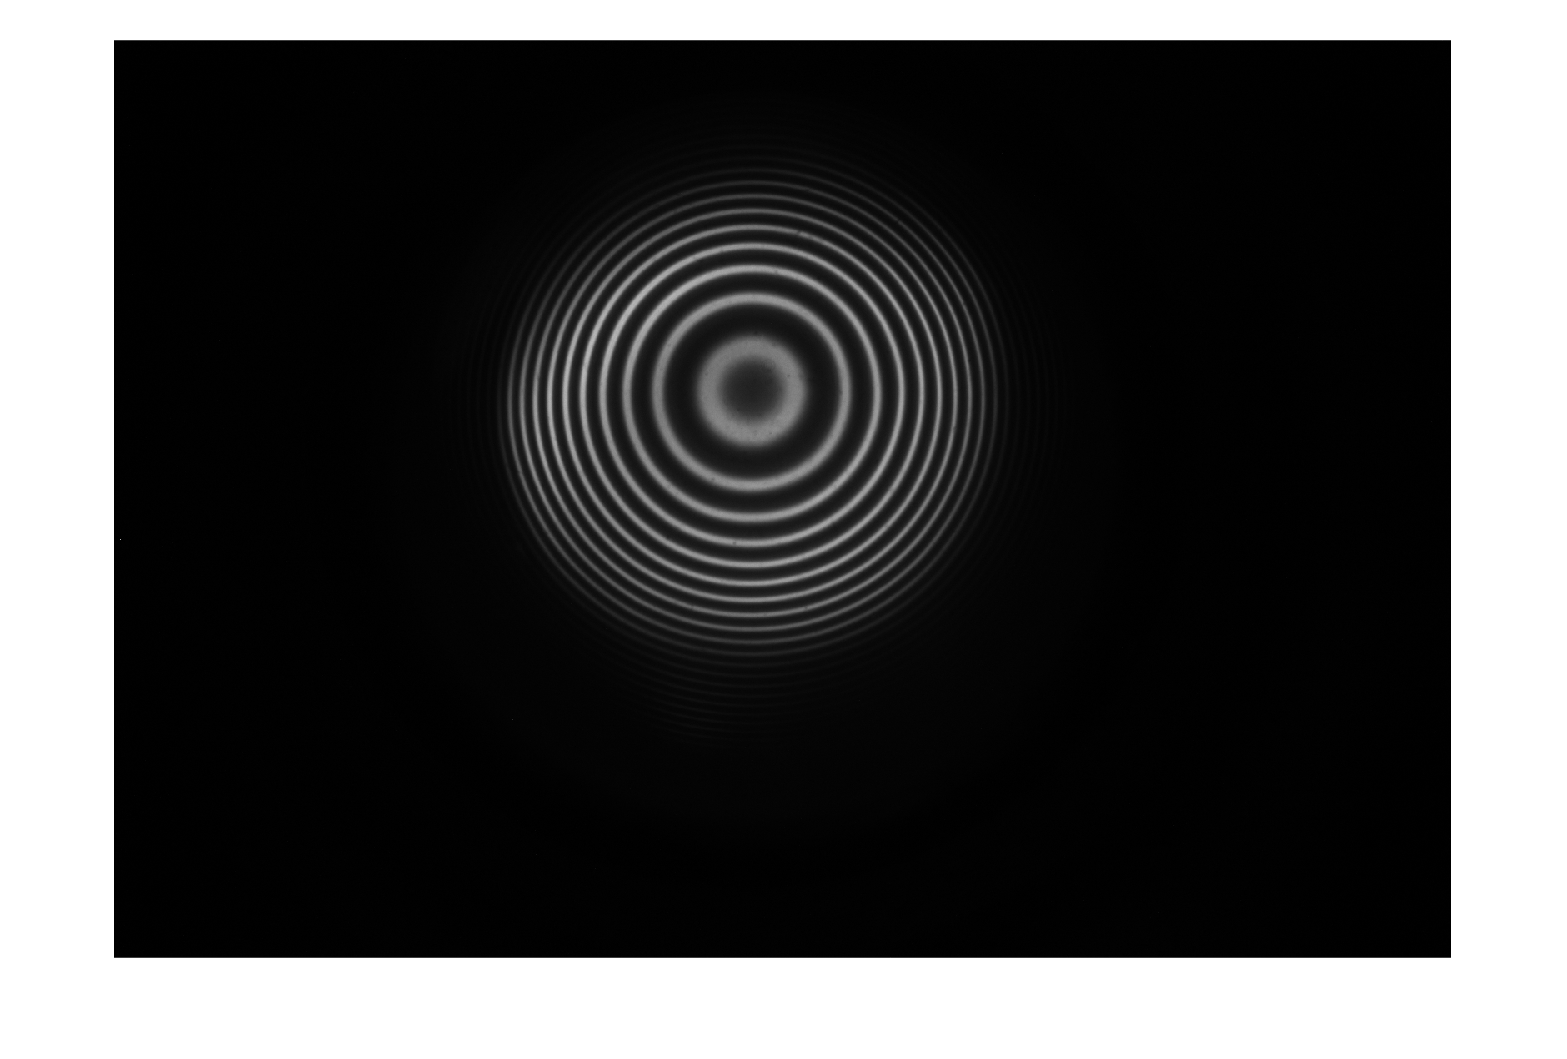
\includegraphics[width=1.2\textwidth]{tra_ano_stripe_hor_53.png}
        \caption{53mm}
      \end{subfigure}
    
      \caption{Observation of transverse anomalous Zeeman effect (Horizontal).}
      \label{fig:tra_ano_hor_fiveimages}
    \end{figure}
    
    \begin{table}[H]
        \centering
        \caption{Radius of transversal anomalous Zeeman effect (Horizontal).}
        \begin{tabular}{c|c|c|c|c|c|c}
            $d $ (mm)& $C1 $ (pixel)& $C2 $ (pixel)& $C3 $ (pixel)& $C4 $ (pixel)& $C5 $ (pixel)& $C6 $ (pixel)\\ \hline \hline
            43&	215.25	&223.5	&233.75	&288.5	&296.25	&304.75 \\ \hline
            45&	218.75	&225	&231.5	&295	&299.75	&305.25 \\ \hline
            48&	220.5	&224.25	&230.5	&295	&299.25	&303.5 \\ \hline
            50& 221	    &224	&229.75	&297	&300	&304 \\ \hline
            53&	222.5	&226.5	&229	&296.5	&298.75	&301.75 \\ \hline
        \end{tabular}
        \label{tab:tra_ano_hor}
    \end{table}
    
    \begin{table}[H]
        \centering
        \caption{Uncertainties of radius of transversal anomalous Zeeman effect (Horizontal).}
        \begin{tabular}{c|c|c|c|c|c|c}
            $d $ (mm)& $u_{C1} $ (pixel)& $u_{C2} $ (pixel)& $u_{C3} $ (pixel)& $u_{C4} $ (pixel)& $u_{C5} $ (pixel)& $u_{C6} $ (pixel) \\ \hline \hline
            43&3.1057&3.3166&3.6940&9.8234&7.8726&6.1083  \\ \hline
            45&3.2882&3.5472&3.5118&4.4253&4.7762&4.9644 \\ \hline
            48&3.5355&4.2204&3.7638&4.3108&5.1295&5.1800  \\ \hline
            50&4.1533&4.2130&3.6940&4.7521&4.9413&5.0414 \\ \hline
            53&3.5118&3.2403&3.5   &4.7784&4.5620&4.8283 \\ \hline
        \end{tabular}
        \label{tab:tra_ano_ver_un}
    \end{table}
    
    \begin{table}[H]
        \centering
        \caption{Side product before the final result, where $\delta_{1}$ is the average of 1 and 2 cells, $\delta_{2}$ is the average of 3 and 4 cells, and $\Delta$ is the average of 5 and 6 and 7 cells.Units are all square of pixel }
        \resizebox{\textwidth}{!}{%
        \begin{tabular}{c|c|c|c|c|c|c|c|c|c|c}
            $d $ (mm)& C2-C1& C3-C2& C5-C4& C6-C5& C4-C1& C5-C2&C6-C3&$\delta_{1}$&$\delta_{2}$&$\Delta$ \\ \hline \hline
            43&11371.58&14724.05&14237.10&16048.82&115923.78&118789.31&120114.08&13047.81&15142.96&118275.72  \\ \hline
            45&8713.01&9321.89&8875.19&10453.64&123066.98&123229.16&124360.92&9017.45&9664.42&123552.35 \\ \hline
            48&5239.587&8928.99&7934.28&8047.77&120652.08&123346.78&122465.56&7084.29&7991.03&122154.80  \\ \hline
            50&4194.02&8196.61&5626.59&7590.08&123678.21&125110.78&124504.26&6195.31&6608.34&124431.08 \\ \hline
            53&5642.30&3577.48&4207.57&5659.57&120656.01&119221.28&121303.37&4609.89&4933.57&120393.55 \\ \hline
        \end{tabular}
        \label{tab:tra_ano_side}
    }
    \end{table}
    
    \begin{table}[H]
        \centering
        \caption{Final result of transversal anomalous Zeeman effect (Vertical).}
        \begin{tabular}{c|c|c|c|c|c|c}
            $d $ (mm)& $B $ (T)& $\frac{\delta_{1}}{\Delta}$ & $\frac{\delta_{2}}{\Delta}$& $u_{B} $ (T)& $u_{\frac{\delta_{1}}{\Delta}} $& $u_{\frac{\delta_{2}}{\Delta}} $ \\ \hline \hline
            43&0.29435&0.11031&0.12803&0.0063519&0.041084&0.12602  \\ \hline
            45&0.23958&0.072984&0.078221&0.0030616&0.039971&0.072463 \\ \hline
            48&0.19281&0.057994&0.065417&0.0011631&0.045753&0.076371  \\ \hline
            50&0.1274&0.049789&0.053108&0.0044667&0.046238&0.074671 \\ \hline        53&0.08443&0.038291&0.040978&0.0019575&0.039877&0.073115 \\ \hline
        \end{tabular}
        \label{tab:tra_ano_final}
    \end{table}
    
    \begin{figure}[H]
        \centering
        \begin{subfigure}[b]{0.48\textwidth}
            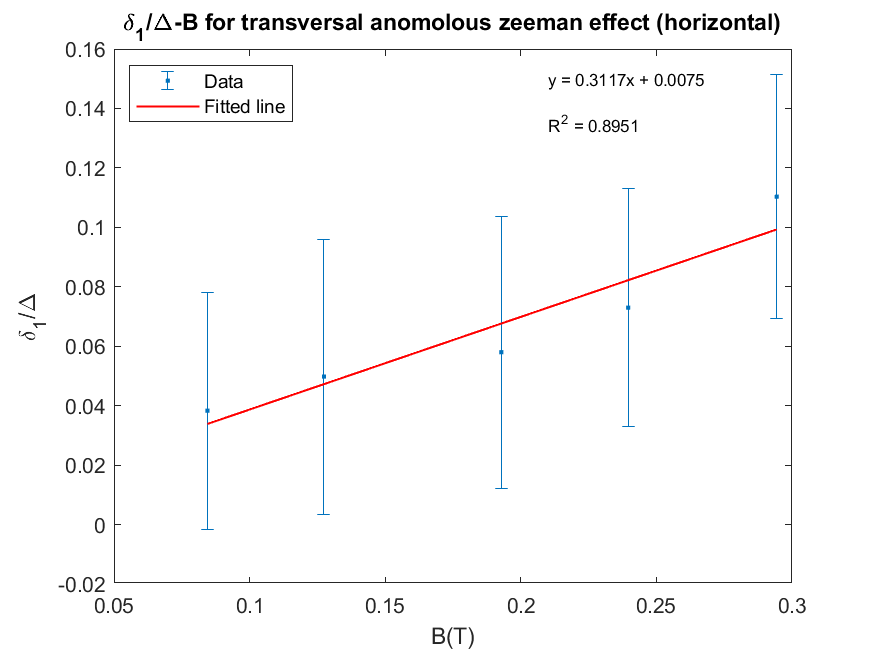
\includegraphics[width=\textwidth]{tra_ano_hor_d1_data.png}
            \caption{Fitting line for $\frac{\delta_{1}}{\Delta}$ with B.}
        \end{subfigure}
        \begin{subfigure}[b]{0.48\textwidth}
            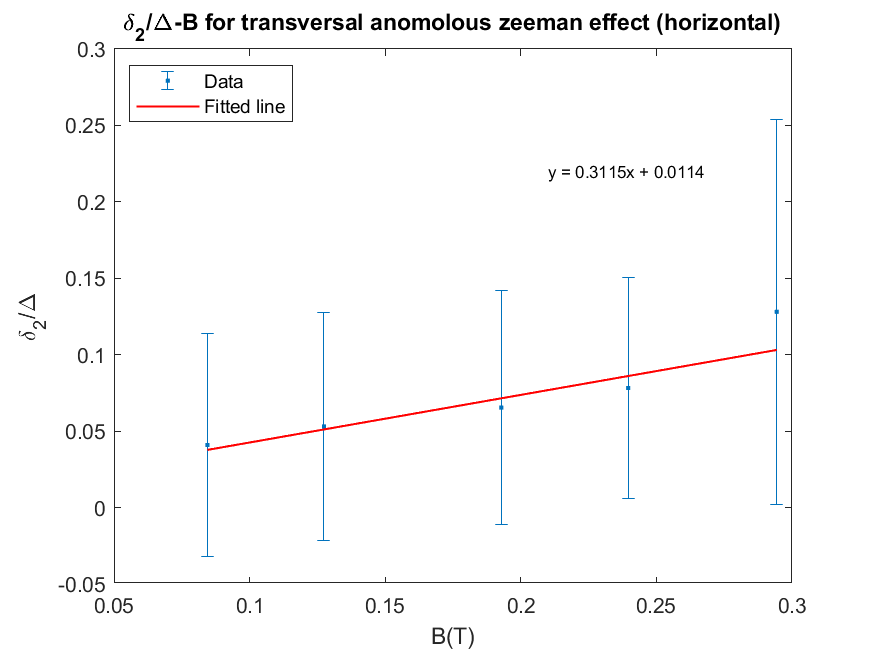
\includegraphics[width=\textwidth]{tra_ano_hor_d2_data.png}
            \caption{Fitting line for $\frac{\delta_{2}}{\Delta}$ with B.}
        \end{subfigure}
        \caption{Fitting line of transversal anomalous Zeeman effect (Horizontal).}
        \label{fig:tra_ano_hor_data}
    \end{figure}
    
    \par The Bohr magneton for this situation is given by Eq.\ref{eq:bohr mag_2}, where $\mu$ = 1.452 and $t$ = 0.003 (m).
    
    \begin{equation}
        \mu_B = \frac{hc}{\mu t} \cdot \frac{\delta}{\Delta B}=\frac{hc}{\mu t} \cdot \text{slope}
        \label{eq:bohr mag_2}  
    \end{equation}
    
    \begin{table}[H]
        \centering
        \caption{Data of transversal anomalous Zeeman effect (Horizontal).}
        \begin{tabular}{c|c|c|c|c|c}
             &slope1 (1/T)& slope2 (1/T)& average slope (1/T)& $\mu_B$ (1/T)& diff \% \\ \hline \hline
            value&0.31175&0.374&0.342875&$1.563619254\cdot 10^{-23}$&0.6862  \\ \hline
            uncertainty&0.24515&0.5219&0.57661&$2.6295215369\cdot 10^{-23}$& \\ \hline
            
        \end{tabular}
        \label{tab:tra_ano_ver_final_data}
    \end{table}
    
    \par From sec.\ref{4.2.2} to sec.\ref{4.2.4} we can see that the error is almost the same degree of magnitude of the value, even larger than the value in the transversal anomalous Zeeman effect (Horizontal). The main reason is the error propagation of the resolution of the CDC-camera, after hundreds of calculations the error is magnified. On the other hand, it also affects the accuracy of the radius for the splitting energy levels. However using Matlab to extract data and Fourier analysis to remove noise indeed reduce the distance to the theoretical value. As long as the resolution of the camera gets better, it is possible for 
     observing a better data.
    
    \section{問題討論}
    \subsection{本實驗選擇鎘燈的原因?}
    \begin{enumerate}
        \item \textbf{Cadmium emits monochromatic spectral lines: }
        Cadmium can emit several spectral light which many of them(especially the red light) are clear to  be observed. 
    
        \item \textbf{Show clear Zeeman splitting under a magnetic field: }
        Under Zeeman effect, Cadmium electrons split into multiple spectral lines, making the observation close to the theoretical prediction.
    
        \item \textbf{High experimental stability: }
        Cadmium lamp provides strong and stable light which is crucial for long time and precise observation.
    
    \end{enumerate}
    
    \subsection{Fabry-Perot的運作原理為何?入射角扮演的意義為何?}
    \par The incident light enters the etalon and reflects between the mirror(fig.\ref{fig:reflection}). For a given incident angle, we can obtain the path difference to calculate the position of the constructive interference eq.\ref{eq:refraction}. After some calculation, the p-th radius is shown in eq.\ref{eq:pth radius}. Noticed that the difference of the radius of two adjacent incident light are constant once the incident angle is fixed. So far, we've shown that Fabry-Perot interferometer generates interference fringes after the incident light passes through, making it easier to observe. According to the fig.\ref{fig:fabry-perot}, different incident angles match to different radius after enter the lens.
    
    
    \begin{align}
        \delta &= \mu (\overline{BC} + \overline{CK}) \\
               &= 2\mu t \cos{\theta} \\
               &= n\lambda
        \label{eq:refraction}
    \end{align}
    
    
    \begin{equation}
        r_p = \sqrt{\frac{2f^2}{n_0} (p-1+ \epsilon)}
        \label{eq:pth radius}
    \end{equation}
    where $t= \overline{BC} \cos{\theta}$, $\mu$ is the refractive index, $n_0 = \frac{2 \overline{BC} \mu \cos{\theta}}{\lambda}$ and $\epsilon$ is constant.
    
    
    \begin{figure}[H]
        \centering
        \begin{minipage}{0.45\textwidth}
            \centering
            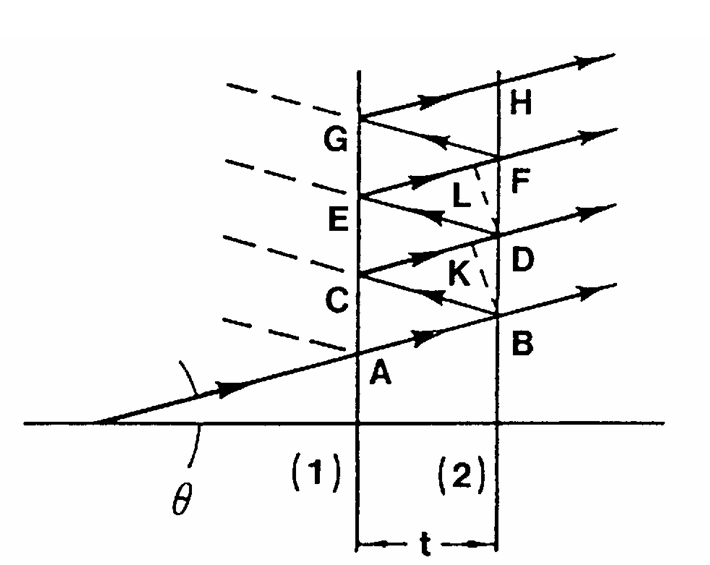
\includegraphics[width=\linewidth]{reflection.png} 
            \caption{}
            \label{fig:reflection}
        \end{minipage}
        \hfill
        \begin{minipage}{0.45\textwidth}
            \centering
            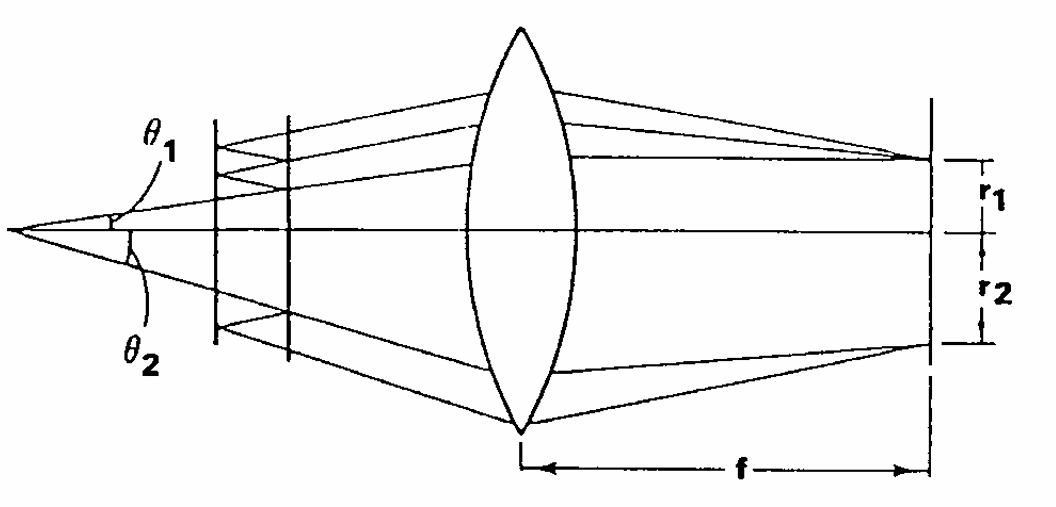
\includegraphics[width=\linewidth]{faby-perot refraction.png}
            \caption{}
            \label{fig:fabry-perot}
        \end{minipage}
    \end{figure}
    
    
    \subsection{$\lambda/4$的玻片在實驗中的意義?}
    \par 
    \begin{itemize}
        \item \textbf{Distinguishing $\pi$ and $\sigma$ spectral lines:} \\
        In the Zeeman effect, energy level splitting under a magnetic field produces different spectral lines ($\pi$, $\sigma^+$, $\sigma^-$) with unique polarization characteristics. These can be observed in specific directions relative to the magnetic field:
    
        \begin{center}
        \begin{tabular}{@{}llll@{}}
        \toprule
        \textbf{Line Type} & \textbf{Transition} & \textbf{Polarization} & \textbf{Observation Direction} \\
        \midrule
        $\pi$ & $\Delta m = 0$ & Linear & Perpendicular to magnetic field \\
        $\sigma^+$ & $\Delta m = +1$ & Left Circular (LCP) & Along the magnetic field \\
        $\sigma^-$ & $\Delta m = -1$ & Right Circular (RCP) & Along the magnetic field \\
        \bottomrule
        \end{tabular}
        \end{center}
    
        Without a QWP, $\sigma^+$ and $\sigma^-$ cannot be distinguished easily because circular polarization is not detectable by the naked eye or standard detectors.
    
        \item \textbf{Conversion to linear polarization:} \\
        The QWP converts circular polarization ($\sigma^+$ or $\sigma^-$) into linear polarization. This allows us to analyze the resulting light using a polarizer and determine the polarization direction, which reveals information about the transition type.
    
        \item \textbf{Facilitating measurement and analysis:} \\
        By combining a QWP and a polarizer, the experiment can:
        \begin{itemize}
            \item Identify whether the spectral line is $\pi$, $\sigma^+$, or $\sigma^-$.
            \item Measure the degree of Zeeman splitting.
            \item Analyze the angular and polarization behavior of emitted light.
        \end{itemize}
    \end{itemize}
    
    
    \subsection{為何能階躍遷不是任意兩能階都可以,說明selection rule的物理機制並推導之}
    \par In Zeeman effect, not all energy level transitions are allowed. Selection rules tell you when a matrix element is zero based on the symmetry of the situation. For the electric dipole transitions, we can use the commutation relation with angular momentum. Then, only two states which follow the eq.\ref{eq:selection rule} are able to be transit.
    
    \begin{align}
        \Delta m &= \pm 1, 0 \\
        \Delta l &= \pm 1, 0
    \label{eq:selection rule}
    \end{align}
    
    
    
    \subsection{四個凸透鏡組跟CCD的用途為何}
    
    \par Convex lenses are commonly used in optical experiment. In this experiment, the main purpose is listed below.
    \begin{enumerate}
        \item Focus the light and control beam path.
    
        \item Ensure collimated or expanded light for better interference.
    
        \item Adjust the optical path length to enhance spectral resolution.
    \end{enumerate}
    
    \par The main use of the CDC system is to capture the subtle image of the interference pattern in this experiment.  
    
    \begin{enumerate}
        \item Captures the interference fringes or spectral patterns caused by the Zeeman effect.
    
        \item Provides high-resolution imaging for detailed analysis of the spectral lines.
    
        \item Allows for digital recording and further analysis of the light's behavior under the influence of a magnetic field.
    \end{enumerate}
    
    \par The convex lenses and the CCD system enable precise control of light and allow clear observation and measurement of the Zeeman effect in the experiment.
    
    \section{Summary} 
    \par In this experiment we observe the normal and anomalous Zeeman effect with the different direction of the magnetic field and the polarization, which result in the different numbers of splitting energy levels and the visible ones on different situation. By picking up certain stripes, we can get the relation between the area of circles and the magnetic field strength, and finally deduce Bohr magneton. However, due to the relatively blurry image, we cannot improve the accuracy, despite having tried a relatively careful method of data extraction.

\section*{References}
\printbibliography

\end{document}